\documentclass{book}
\usepackage[a4paper,top=2.5cm,bottom=2.5cm,left=2.5cm,right=2.5cm]{geometry}
\usepackage{makeidx}
\usepackage{natbib}
\usepackage{graphicx}
\usepackage{multicol}
\usepackage{float}
\usepackage{listings}
\usepackage{color}
\usepackage{ifthen}
\usepackage[table]{xcolor}
\usepackage{textcomp}
\usepackage{alltt}
\usepackage{ifpdf}
\ifpdf
\usepackage[pdftex,
            pagebackref=true,
            colorlinks=true,
            linkcolor=blue,
            unicode
           ]{hyperref}
\else
\usepackage[ps2pdf,
            pagebackref=true,
            colorlinks=true,
            linkcolor=blue,
            unicode
           ]{hyperref}
\usepackage{pspicture}
\fi
\usepackage[utf8]{inputenc}
\usepackage{mathptmx}
\usepackage[scaled=.90]{helvet}
\usepackage{courier}
\usepackage{sectsty}
\usepackage[titles]{tocloft}
\usepackage{doxygen}
\lstset{language=C++,inputencoding=utf8,basicstyle=\footnotesize,breaklines=true,breakatwhitespace=true,tabsize=9,numbers=left }
\makeindex
\setcounter{tocdepth}{3}
\renewcommand{\footrulewidth}{0.4pt}
\renewcommand{\familydefault}{\sfdefault}
\hfuzz=15pt
\setlength{\emergencystretch}{15pt}
\hbadness=750
\tolerance=750
\begin{document}
\hypersetup{pageanchor=false,citecolor=blue}
\begin{titlepage}
\vspace*{7cm}
\begin{center}
{\Large Ez2\-D\-S \\[1ex]\large In Development }\\
\vspace*{1cm}
{\large Generated by Doxygen 1.8.0}\\
\vspace*{0.5cm}
{\small Wed Apr 25 2012 00:15:09}\\
\end{center}
\end{titlepage}
\clearemptydoublepage
\pagenumbering{roman}
\tableofcontents
\clearemptydoublepage
\pagenumbering{arabic}
\hypersetup{pageanchor=true,citecolor=blue}
\chapter{Module Index}
\section{Modules}
Here is a list of all modules\-:\begin{DoxyCompactList}
\item \contentsline{section}{E2d\-Element}{\pageref{group__e2dElement}}{}
\item \contentsline{section}{E2d\-Group}{\pageref{group__e2dGroup}}{}
\item \contentsline{section}{E2d\-Image}{\pageref{group__e2dImage}}{}
\item \contentsline{section}{E2d\-Matrix}{\pageref{group__e2dMatrix}}{}
\item \contentsline{section}{E2d\-Point}{\pageref{group__e2dPoint}}{}
\item \contentsline{section}{E2d\-Scene}{\pageref{group__e2dScene}}{}
\end{DoxyCompactList}

\chapter{Data Structure Index}
\section{Data Structures}
Here are the data structures with brief descriptions\-:\begin{DoxyCompactList}
\item\contentsline{section}{\hyperlink{structe2dElement}{e2d\-Element} \\*The \hyperlink{structe2dElement}{e2d\-Element} struct is the base of all elements in the scene. Common scene information such as id, attribute values or transformations are saved in the \hyperlink{structe2dElement}{e2d\-Element} struct. You are not meant to instance this struct by itself. By creating other elements such as \hyperlink{structe2dGroup}{e2d\-Group} or \hyperlink{structe2dImage}{e2d\-Image}, this struct will be automatically allocated in them. This \char`\"{}inheritance\char`\"{} is mimic'd by placing the \hyperlink{structe2dElement}{e2d\-Element} struct as the first element in structs which are meant to be \char`\"{}substructs\char`\"{} of it }{\pageref{structe2dElement}}{}
\item\contentsline{section}{\hyperlink{structe2dGroup}{e2d\-Group} \\*The \hyperlink{structe2dGroup}{e2d\-Group} struct is used to group elements in the scene. This struct is created from the \char`\"{}g\char`\"{} element in S\-V\-G. It \char`\"{}inherits\char`\"{} from \hyperlink{structe2dElement}{e2d\-Element} by placing it as the first element in the struct, if you typecast e2d\-Group$\ast$ into e2d\-Element$\ast$, it will work thus mimicing inheritance in e.\-g. C++ }{\pageref{structe2dGroup}}{}
\item\contentsline{section}{\hyperlink{structe2dGroupIterator}{e2d\-Group\-Iterator} \\*An iterator for the children of \hyperlink{structe2dGroup}{e2d\-Group} }{\pageref{structe2dGroupIterator}}{}
\item\contentsline{section}{\hyperlink{structe2dImage}{e2d\-Image} \\*The \hyperlink{structe2dImage}{e2d\-Image} struct is used for holding the paths to images and their size and position. The struct is composed directly from the contents of the S\-V\-G image element. It \char`\"{}inherits\char`\"{} from \hyperlink{structe2dElement}{e2d\-Element} by placing it as the first element in the struct, if you typecast e2d\-Image$\ast$ into e2d\-Element$\ast$, it will work thus mimicing inheritance in e.\-g. C++ }{\pageref{structe2dImage}}{}
\item\contentsline{section}{\hyperlink{structe2dMatrix}{e2d\-Matrix} \\*The \hyperlink{structe2dMatrix}{e2d\-Matrix} struct contains the implementation of a 3x3 matrix which is row major. See \href{http://en.wikipedia.org/wiki/Row-major_order}{\tt http\-://en.\-wikipedia.\-org/wiki/\-Row-\/major\-\_\-order} if you have doubts }{\pageref{structe2dMatrix}}{}
\item\contentsline{section}{\hyperlink{structe2dPath}{e2d\-Path} \\*The \hyperlink{structe2dPath}{e2d\-Path} struct is used for holding the information of path. The struct is composed directly from the contents of the S\-V\-G path element. It \char`\"{}inherits\char`\"{} from \hyperlink{structe2dElement}{e2d\-Element} by placing it as the first element in the struct, if you typecast e2d\-Path$\ast$ into e2d\-Element$\ast$, it will work thus mimicing inheritance in e.\-g. C++ }{\pageref{structe2dPath}}{}
\item\contentsline{section}{\hyperlink{structe2dPathCurve}{e2d\-Path\-Curve} \\*This struct represents a curve in the path. It is a cubic bezier curve, having two control points. It \char`\"{}inherits\char`\"{} from \hyperlink{structe2dPathElement}{e2d\-Path\-Element} by placing it as the first element in the struct, if you typecast e2d\-Path\-Point$\ast$ into e2d\-Path\-Element$\ast$, it will work thus mimicing inheritance in e.\-g. C++ }{\pageref{structe2dPathCurve}}{}
\item\contentsline{section}{\hyperlink{structe2dPathElement}{e2d\-Path\-Element} \\*The \hyperlink{structe2dPathElement}{e2d\-Path\-Element} is the \char`\"{}super struct\char`\"{} of all path elements in the scene. Its inheritting functionality works in much the same way as \hyperlink{structe2dElement}{e2d\-Element}, so you should look into it to understand. }{\pageref{structe2dPathElement}}{}
\item\contentsline{section}{\hyperlink{structe2dPathElementIterator}{e2d\-Path\-Element\-Iterator} \\*An iterator for the path elements }{\pageref{structe2dPathElementIterator}}{}
\item\contentsline{section}{\hyperlink{structe2dPathPoint}{e2d\-Path\-Point} \\*This struct represents a point in the path. It \char`\"{}inherits\char`\"{} from \hyperlink{structe2dPathElement}{e2d\-Path\-Element} by placing it as the first element in the struct, if you typecast e2d\-Path\-Point$\ast$ into e2d\-Path\-Element$\ast$, it will work thus mimicing inheritance in e.\-g. C++ }{\pageref{structe2dPathPoint}}{}
\item\contentsline{section}{\hyperlink{structe2dPoint}{e2d\-Point} \\*The \hyperlink{structe2dPoint}{e2d\-Point} struct which contains two floats }{\pageref{structe2dPoint}}{}
\item\contentsline{section}{\hyperlink{structe2dScene}{e2d\-Scene} \\*The \hyperlink{structe2dScene}{e2d\-Scene} struct defines a scene obtained from an S\-V\-G file. The struct contains the root under which all the objects in the scene can be accessed }{\pageref{structe2dScene}}{}
\item\contentsline{section}{\hyperlink{structe2dSceneSearchResult}{e2d\-Scene\-Search\-Result} \\*This struct represents the results returns by e2d\-Scene\-Search. You should always destroy the result with \hyperlink{group__e2dScene_ga0eedd7c50a3d65e91abd54fcee3de39d}{e2d\-Scene\-Search\-Result\-Destroy()} }{\pageref{structe2dSceneSearchResult}}{}
\end{DoxyCompactList}

\chapter{File Index}
\section{File List}
Here is a list of all documented files with brief descriptions\-:\begin{DoxyCompactList}
\item\contentsline{section}{\hyperlink{e2dElement_8h}{e2d\-Element.\-h} \\*File which contains the \hyperlink{structe2dElement}{e2d\-Element} struct and its \char`\"{}methods\char`\"{} }{\pageref{e2dElement_8h}}{}
\item\contentsline{section}{\hyperlink{e2dGroup_8h}{e2d\-Group.\-h} \\*File which contains the \hyperlink{structe2dGroup}{e2d\-Group} struct and its \char`\"{}methods\char`\"{} }{\pageref{e2dGroup_8h}}{}
\item\contentsline{section}{\hyperlink{e2dImage_8h}{e2d\-Image.\-h} \\*File which contains the \hyperlink{structe2dImage}{e2d\-Image} struct and its \char`\"{}methods\char`\"{} }{\pageref{e2dImage_8h}}{}
\item\contentsline{section}{\hyperlink{e2dMatrix_8h}{e2d\-Matrix.\-h} \\*File which contains a 3x3 matrix implementation and utility methods }{\pageref{e2dMatrix_8h}}{}
\item\contentsline{section}{{\bfseries e2d\-Path.\-h} }{\pageref{e2dPath_8h}}{}
\item\contentsline{section}{\hyperlink{e2dPoint_8h}{e2d\-Point.\-h} \\*File which contains a struct definition of a point (two floats) }{\pageref{e2dPoint_8h}}{}
\item\contentsline{section}{\hyperlink{e2dScene_8h}{e2d\-Scene.\-h} \\*File which contains the \hyperlink{structe2dScene}{e2d\-Scene} struct and its \char`\"{}methods\char`\"{} }{\pageref{e2dScene_8h}}{}
\item\contentsline{section}{\hyperlink{Ez2DS_8h}{Ez2\-D\-S.\-h} \\*File which contains global definitions useful to be included on every other file of the library. These definitions include forward declaration of all the structs, and some utility functions }{\pageref{Ez2DS_8h}}{}
\end{DoxyCompactList}

\chapter{Module Documentation}
\hypertarget{group__e2dElement}{\section{E2d\-Element}
\label{group__e2dElement}\index{E2d\-Element@{E2d\-Element}}
}
\subsection*{Data Structures}
\begin{DoxyCompactItemize}
\item 
struct \hyperlink{structe2dElement}{e2d\-Element}
\begin{DoxyCompactList}\small\item\em The \hyperlink{structe2dElement}{e2d\-Element} struct is the base of all elements in the scene. Common scene information such as id, attribute values or transformations are saved in the \hyperlink{structe2dElement}{e2d\-Element} struct. You are not meant to instance this struct by itself. By creating other elements such as \hyperlink{structe2dGroup}{e2d\-Group} or \hyperlink{structe2dImage}{e2d\-Image}, this struct will be automatically allocated in them. This \char`\"{}inheritance\char`\"{} is mimic'd by placing the \hyperlink{structe2dElement}{e2d\-Element} struct as the first element in structs which are meant to be \char`\"{}substructs\char`\"{} of it. \end{DoxyCompactList}\end{DoxyCompactItemize}
\subsection*{Typedefs}
\begin{DoxyCompactItemize}
\item 
\hypertarget{group__e2dElement_ga13e962cd8fa5eaa7d4bec3fc7d774d59}{typedef enum \hyperlink{group__e2dElement_ga9bc8cfdec08c7e9069fc707ee456fd38}{e2d\-Element\-Type} \hyperlink{group__e2dElement_ga13e962cd8fa5eaa7d4bec3fc7d774d59}{e2d\-Element\-Type}}\label{group__e2dElement_ga13e962cd8fa5eaa7d4bec3fc7d774d59}

\begin{DoxyCompactList}\small\item\em The e2d\-Element\-Type enum defines the possible \char`\"{}substructs\char`\"{} of \hyperlink{structe2dElement}{e2d\-Element}. This is used for reflection. \end{DoxyCompactList}\end{DoxyCompactItemize}
\subsection*{Enumerations}
\begin{DoxyCompactItemize}
\item 
enum \hyperlink{group__e2dElement_ga9bc8cfdec08c7e9069fc707ee456fd38}{e2d\-Element\-Type} \{ {\bfseries E2\-D\-\_\-\-G\-R\-O\-U\-P}, 
{\bfseries E2\-D\-\_\-\-P\-A\-T\-H}, 
{\bfseries E2\-D\-\_\-\-I\-M\-A\-G\-E}
 \}
\begin{DoxyCompactList}\small\item\em The e2d\-Element\-Type enum defines the possible \char`\"{}substructs\char`\"{} of \hyperlink{structe2dElement}{e2d\-Element}. This is used for reflection. \end{DoxyCompactList}\end{DoxyCompactItemize}
\subsection*{Functions}
\begin{DoxyCompactItemize}
\item 
void \hyperlink{group__e2dElement_ga8734d10ef40a380dfc51bfe1790a92a7}{e2d\-Element\-Init} (\hyperlink{structe2dElement}{e2d\-Element} $\ast$element, \hyperlink{group__e2dElement_ga9bc8cfdec08c7e9069fc707ee456fd38}{e2d\-Element\-Type} type, const \hyperlink{structe2dScene}{e2d\-Scene} $\ast$scene)
\begin{DoxyCompactList}\small\item\em Called by the create methods of structs which inherit \hyperlink{structe2dElement}{e2d\-Element} (e.\-g. e2d\-Group\-Create). Will initialize all members of the struct with the parameters of this method and with default values on everything else. \end{DoxyCompactList}\item 
void \hyperlink{group__e2dElement_ga214c437a16fe6f3fc795539f851a2019}{e2d\-Element\-Destroy} (\hyperlink{structe2dElement}{e2d\-Element} $\ast$elem)
\begin{DoxyCompactList}\small\item\em Will check the type member of elem and call the appropriate destructor (e.\-g. \hyperlink{group__e2dGroup_ga545626effa0f89b72f244e56aadb05bc}{e2d\-Group\-Destroy()}) \end{DoxyCompactList}\item 
void \hyperlink{group__e2dElement_gae8da5104d70a09549ca74044dda8313c}{e2d\-Element\-Free\-Members} (\hyperlink{structe2dElement}{e2d\-Element} $\ast$elem)
\begin{DoxyCompactList}\small\item\em Will free all the allocated memory inside the \hyperlink{structe2dElement}{e2d\-Element} struct pointed by elem. \end{DoxyCompactList}\item 
void \hyperlink{group__e2dElement_ga5cfa0a343d3dd1a30b0addc4ec6e7f88}{e2d\-Element\-Add\-Attribute} (\hyperlink{structe2dElement}{e2d\-Element} $\ast$elem, const char $\ast$name, const char $\ast$value)
\begin{DoxyCompactList}\small\item\em Will add an attribute to the element. Increases the size of the array if necessary. \end{DoxyCompactList}\item 
const char $\ast$ \hyperlink{group__e2dElement_gac32ea8a33b317fc014929102d64ac157}{e2d\-Element\-Get\-Attribute} (\hyperlink{structe2dElement}{e2d\-Element} $\ast$elem, const char $\ast$name)
\begin{DoxyCompactList}\small\item\em Returns the value of an attribute with a given name. \end{DoxyCompactList}\item 
\hyperlink{structe2dPoint}{e2d\-Point} \hyperlink{group__e2dElement_ga39dd883e42f609efba3f75300a29ff31}{e2d\-Element\-Get\-Local\-Position} (const \hyperlink{structe2dElement}{e2d\-Element} $\ast$elem)
\begin{DoxyCompactList}\small\item\em Returns the position of the element, taken from the local\-Transform. \end{DoxyCompactList}\item 
\hyperlink{structe2dPoint}{e2d\-Point} \hyperlink{group__e2dElement_ga9b85de42e52c0d89e82f9231ea923c8c}{e2d\-Element\-Get\-World\-Position} (const \hyperlink{structe2dElement}{e2d\-Element} $\ast$elem)
\begin{DoxyCompactList}\small\item\em U\-N\-T\-E\-S\-T\-E\-D Will get the local position (\hyperlink{group__e2dElement_ga39dd883e42f609efba3f75300a29ff31}{e2d\-Element\-Get\-Local\-Position()}) and multiply it by the inverse\-Effective\-Transform and obtain the world position. Needs effective transformations to be calculated ( e2d\-Scene\-Calculate\-Effective\-Transforms() has been called) \end{DoxyCompactList}\item 
\hyperlink{structe2dPoint}{e2d\-Point} \hyperlink{group__e2dElement_gab4e3f4eeba31c937a946f68617c5cb06}{e2d\-Element\-Get\-Relative\-Position} (const \hyperlink{structe2dElement}{e2d\-Element} $\ast$elem, const \hyperlink{structe2dElement}{e2d\-Element} $\ast$relative\-To)
\begin{DoxyCompactList}\small\item\em U\-N\-T\-E\-S\-T\-E\-D Will get the relative transformation by multiplying the effective transform of elem with the inverse effective transform of relative\-To. The multiply it with the local position of elem (\hyperlink{group__e2dElement_ga39dd883e42f609efba3f75300a29ff31}{e2d\-Element\-Get\-Local\-Position()}). Needs effective transformations to be calculated (e2d\-Scene\-Calculate\-Effective\-Transforms() has been called) \end{DoxyCompactList}\item 
\hyperlink{structe2dPoint}{e2d\-Point} \hyperlink{group__e2dElement_gac3ad9f8cdc0782378c9f2e93cb7da68f}{e2d\-Element\-Get\-Relative\-Point} (const \hyperlink{structe2dElement}{e2d\-Element} $\ast$elem, const \hyperlink{structe2dElement}{e2d\-Element} $\ast$relative\-To, const \hyperlink{structe2dPoint}{e2d\-Point} $\ast$point)
\begin{DoxyCompactList}\small\item\em U\-N\-T\-E\-S\-T\-E\-D Will get the relative transformation by multiplying the effective transform of elem with the inverse effective transform of relative\-To. The multiply it with point. Needs effective transformations to be calculated (e2d\-Scene\-Calculate\-Effective\-Transforms() has been called). \end{DoxyCompactList}\item 
void \hyperlink{group__e2dElement_ga94aa710b2da71af2091fe4d5b87ce47e}{e2d\-Element\-Calculate\-Bounding\-Box} (\hyperlink{structe2dElement}{e2d\-Element} $\ast$elem)
\begin{DoxyCompactList}\small\item\em Will check type and calculate the appropriate method (e.\-g. \hyperlink{group__e2dGroup_ga7c5f43489bbd2d36a51414aee07abf5a}{e2d\-Group\-Calculate\-Bounding\-Box()}) \end{DoxyCompactList}\item 
void \hyperlink{group__e2dElement_ga36b01a888c97163c990e16d348aff61c}{e2d\-Element\-Center\-At\-B\-Box} (\hyperlink{structe2dElement}{e2d\-Element} $\ast$elem, float tx, float ty)
\begin{DoxyCompactList}\small\item\em Needs bounding box to have been calculated. Will check type and calculate the appropriate method (e.\-g. \hyperlink{group__e2dGroup_ga04bf94419865ca7f9d6daf30ce3fadf0}{e2d\-Group\-Center\-At\-B\-Box()}). (tx, ty) will define where in the bounding box, the element will be centered, e.\-g. (0,0, will center on the top left corner, (0.\-5, 0.\-5) will center on the center of the bbox. \end{DoxyCompactList}\end{DoxyCompactItemize}


\subsection{Function Documentation}
\hypertarget{group__e2dElement_ga5cfa0a343d3dd1a30b0addc4ec6e7f88}{\index{E2d\-Element@{E2d\-Element}!e2d\-Element\-Add\-Attribute@{e2d\-Element\-Add\-Attribute}}
\index{e2d\-Element\-Add\-Attribute@{e2d\-Element\-Add\-Attribute}!E2dElement@{E2d\-Element}}
\subsubsection[{e2d\-Element\-Add\-Attribute}]{\setlength{\rightskip}{0pt plus 5cm}void {\bf e2d\-Element\-Add\-Attribute} (
\begin{DoxyParamCaption}
\item[{{\bf e2d\-Element} $\ast$}]{elem, }
\item[{const char $\ast$}]{name, }
\item[{const char $\ast$}]{value}
\end{DoxyParamCaption}
)}}\label{group__e2dElement_ga5cfa0a343d3dd1a30b0addc4ec6e7f88}


Will add an attribute to the element. Increases the size of the array if necessary. 


\begin{DoxyParams}[1]{Parameters}
\mbox{\tt in}  & {\em elem} & The \hyperlink{structe2dElement}{e2d\-Element} where the attribute will be added. \\
\hline
\mbox{\tt in}  & {\em name} & The name of the attribute. \\
\hline
\mbox{\tt in}  & {\em value} & The value of the attribute. \\
\hline
\end{DoxyParams}
\hypertarget{group__e2dElement_ga94aa710b2da71af2091fe4d5b87ce47e}{\index{E2d\-Element@{E2d\-Element}!e2d\-Element\-Calculate\-Bounding\-Box@{e2d\-Element\-Calculate\-Bounding\-Box}}
\index{e2d\-Element\-Calculate\-Bounding\-Box@{e2d\-Element\-Calculate\-Bounding\-Box}!E2dElement@{E2d\-Element}}
\subsubsection[{e2d\-Element\-Calculate\-Bounding\-Box}]{\setlength{\rightskip}{0pt plus 5cm}void {\bf e2d\-Element\-Calculate\-Bounding\-Box} (
\begin{DoxyParamCaption}
\item[{{\bf e2d\-Element} $\ast$}]{elem}
\end{DoxyParamCaption}
)}}\label{group__e2dElement_ga94aa710b2da71af2091fe4d5b87ce47e}


Will check type and calculate the appropriate method (e.\-g. \hyperlink{group__e2dGroup_ga7c5f43489bbd2d36a51414aee07abf5a}{e2d\-Group\-Calculate\-Bounding\-Box()}) 


\begin{DoxyParams}[1]{Parameters}
\mbox{\tt in}  & {\em elem} & The \hyperlink{structe2dElement}{e2d\-Element} to calculate.\\
\hline
\end{DoxyParams}
\begin{DoxySeeAlso}{See also}
\hyperlink{group__e2dGroup_ga7c5f43489bbd2d36a51414aee07abf5a}{e2d\-Group\-Calculate\-Bounding\-Box()} 

\hyperlink{group__e2dImage_ga6df4ef2b71e130f5817b079b6b32d249}{e2d\-Image\-Calculate\-Bounding\-Box()} 

e2d\-Path\-Calculate\-Bounding\-Box() 
\end{DoxySeeAlso}
\hypertarget{group__e2dElement_ga36b01a888c97163c990e16d348aff61c}{\index{E2d\-Element@{E2d\-Element}!e2d\-Element\-Center\-At\-B\-Box@{e2d\-Element\-Center\-At\-B\-Box}}
\index{e2d\-Element\-Center\-At\-B\-Box@{e2d\-Element\-Center\-At\-B\-Box}!E2dElement@{E2d\-Element}}
\subsubsection[{e2d\-Element\-Center\-At\-B\-Box}]{\setlength{\rightskip}{0pt plus 5cm}void {\bf e2d\-Element\-Center\-At\-B\-Box} (
\begin{DoxyParamCaption}
\item[{{\bf e2d\-Element} $\ast$}]{elem, }
\item[{float}]{tx, }
\item[{float}]{ty}
\end{DoxyParamCaption}
)}}\label{group__e2dElement_ga36b01a888c97163c990e16d348aff61c}


Needs bounding box to have been calculated. Will check type and calculate the appropriate method (e.\-g. \hyperlink{group__e2dGroup_ga04bf94419865ca7f9d6daf30ce3fadf0}{e2d\-Group\-Center\-At\-B\-Box()}). (tx, ty) will define where in the bounding box, the element will be centered, e.\-g. (0,0, will center on the top left corner, (0.\-5, 0.\-5) will center on the center of the bbox. 


\begin{DoxyParams}[1]{Parameters}
\mbox{\tt in}  & {\em elem} & The \hyperlink{structe2dElement}{e2d\-Element} to center. \\
\hline
\mbox{\tt in}  & {\em tx} & x offset in B\-Box width units. \\
\hline
\mbox{\tt in}  & {\em ty} & y offset in B\-Box height units.\\
\hline
\end{DoxyParams}
\begin{DoxySeeAlso}{See also}
\hyperlink{group__e2dElement_ga94aa710b2da71af2091fe4d5b87ce47e}{e2d\-Element\-Calculate\-Bounding\-Box()} 

\hyperlink{group__e2dGroup_ga04bf94419865ca7f9d6daf30ce3fadf0}{e2d\-Group\-Center\-At\-B\-Box()} 

\hyperlink{group__e2dImage_ga08652fd1ad70d4935d98bcc02a38fb69}{e2d\-Image\-Center\-At\-B\-Box()} 

e2d\-Path\-Center\-At\-B\-Box() 
\end{DoxySeeAlso}
\hypertarget{group__e2dElement_ga214c437a16fe6f3fc795539f851a2019}{\index{E2d\-Element@{E2d\-Element}!e2d\-Element\-Destroy@{e2d\-Element\-Destroy}}
\index{e2d\-Element\-Destroy@{e2d\-Element\-Destroy}!E2dElement@{E2d\-Element}}
\subsubsection[{e2d\-Element\-Destroy}]{\setlength{\rightskip}{0pt plus 5cm}void {\bf e2d\-Element\-Destroy} (
\begin{DoxyParamCaption}
\item[{{\bf e2d\-Element} $\ast$}]{elem}
\end{DoxyParamCaption}
)}}\label{group__e2dElement_ga214c437a16fe6f3fc795539f851a2019}


Will check the type member of elem and call the appropriate destructor (e.\-g. \hyperlink{group__e2dGroup_ga545626effa0f89b72f244e56aadb05bc}{e2d\-Group\-Destroy()}) 


\begin{DoxyParams}[1]{Parameters}
\mbox{\tt in}  & {\em elem} & The \hyperlink{structe2dElement}{e2d\-Element} to be destroyed.\\
\hline
\end{DoxyParams}
\begin{DoxySeeAlso}{See also}
\hyperlink{group__e2dGroup_ga545626effa0f89b72f244e56aadb05bc}{e2d\-Group\-Destroy()} 

\hyperlink{group__e2dImage_gacf174e48578f0e23888e37f47a3ef10b}{e2d\-Image\-Destroy()} 

e2d\-Path\-Destroy() 
\end{DoxySeeAlso}
\hypertarget{group__e2dElement_gae8da5104d70a09549ca74044dda8313c}{\index{E2d\-Element@{E2d\-Element}!e2d\-Element\-Free\-Members@{e2d\-Element\-Free\-Members}}
\index{e2d\-Element\-Free\-Members@{e2d\-Element\-Free\-Members}!E2dElement@{E2d\-Element}}
\subsubsection[{e2d\-Element\-Free\-Members}]{\setlength{\rightskip}{0pt plus 5cm}void {\bf e2d\-Element\-Free\-Members} (
\begin{DoxyParamCaption}
\item[{{\bf e2d\-Element} $\ast$}]{elem}
\end{DoxyParamCaption}
)}}\label{group__e2dElement_gae8da5104d70a09549ca74044dda8313c}


Will free all the allocated memory inside the \hyperlink{structe2dElement}{e2d\-Element} struct pointed by elem. 


\begin{DoxyParams}[1]{Parameters}
\mbox{\tt in}  & {\em elem} & The \hyperlink{structe2dElement}{e2d\-Element} struct where the members will be freed. \\
\hline
\end{DoxyParams}
\hypertarget{group__e2dElement_gac32ea8a33b317fc014929102d64ac157}{\index{E2d\-Element@{E2d\-Element}!e2d\-Element\-Get\-Attribute@{e2d\-Element\-Get\-Attribute}}
\index{e2d\-Element\-Get\-Attribute@{e2d\-Element\-Get\-Attribute}!E2dElement@{E2d\-Element}}
\subsubsection[{e2d\-Element\-Get\-Attribute}]{\setlength{\rightskip}{0pt plus 5cm}const char$\ast$ {\bf e2d\-Element\-Get\-Attribute} (
\begin{DoxyParamCaption}
\item[{{\bf e2d\-Element} $\ast$}]{elem, }
\item[{const char $\ast$}]{name}
\end{DoxyParamCaption}
)}}\label{group__e2dElement_gac32ea8a33b317fc014929102d64ac157}


Returns the value of an attribute with a given name. 


\begin{DoxyParams}[1]{Parameters}
\mbox{\tt in}  & {\em elem} & The \hyperlink{structe2dElement}{e2d\-Element} containing the attribute. \\
\hline
\mbox{\tt in}  & {\em name} & The name of the attribute.\\
\hline
\end{DoxyParams}

\begin{DoxyRetVals}{Return values}
{\em const} & char$\ast$ The value of the name. Null if not found. \\
\hline
\end{DoxyRetVals}
\hypertarget{group__e2dElement_ga39dd883e42f609efba3f75300a29ff31}{\index{E2d\-Element@{E2d\-Element}!e2d\-Element\-Get\-Local\-Position@{e2d\-Element\-Get\-Local\-Position}}
\index{e2d\-Element\-Get\-Local\-Position@{e2d\-Element\-Get\-Local\-Position}!E2dElement@{E2d\-Element}}
\subsubsection[{e2d\-Element\-Get\-Local\-Position}]{\setlength{\rightskip}{0pt plus 5cm}{\bf e2d\-Point} {\bf e2d\-Element\-Get\-Local\-Position} (
\begin{DoxyParamCaption}
\item[{const {\bf e2d\-Element} $\ast$}]{elem}
\end{DoxyParamCaption}
)}}\label{group__e2dElement_ga39dd883e42f609efba3f75300a29ff31}


Returns the position of the element, taken from the local\-Transform. 


\begin{DoxyParams}[1]{Parameters}
\mbox{\tt in}  & {\em elem} & The \hyperlink{structe2dElement}{e2d\-Element} where the position will be requested.\\
\hline
\end{DoxyParams}

\begin{DoxyRetVals}{Return values}
{\em \hyperlink{structe2dPoint}{e2d\-Point}} & The position. \\
\hline
\end{DoxyRetVals}
\hypertarget{group__e2dElement_gac3ad9f8cdc0782378c9f2e93cb7da68f}{\index{E2d\-Element@{E2d\-Element}!e2d\-Element\-Get\-Relative\-Point@{e2d\-Element\-Get\-Relative\-Point}}
\index{e2d\-Element\-Get\-Relative\-Point@{e2d\-Element\-Get\-Relative\-Point}!E2dElement@{E2d\-Element}}
\subsubsection[{e2d\-Element\-Get\-Relative\-Point}]{\setlength{\rightskip}{0pt plus 5cm}{\bf e2d\-Point} {\bf e2d\-Element\-Get\-Relative\-Point} (
\begin{DoxyParamCaption}
\item[{const {\bf e2d\-Element} $\ast$}]{elem, }
\item[{const {\bf e2d\-Element} $\ast$}]{relative\-To, }
\item[{const {\bf e2d\-Point} $\ast$}]{point}
\end{DoxyParamCaption}
)}}\label{group__e2dElement_gac3ad9f8cdc0782378c9f2e93cb7da68f}


U\-N\-T\-E\-S\-T\-E\-D Will get the relative transformation by multiplying the effective transform of elem with the inverse effective transform of relative\-To. The multiply it with point. Needs effective transformations to be calculated (e2d\-Scene\-Calculate\-Effective\-Transforms() has been called). 


\begin{DoxyParams}[1]{Parameters}
\mbox{\tt in}  & {\em elem} & The \hyperlink{structe2dElement}{e2d\-Element} where the position will be requested. \\
\hline
\mbox{\tt in}  & {\em relative\-To} & The result will be relative to this \hyperlink{structe2dElement}{e2d\-Element}.\\
\hline
\end{DoxyParams}

\begin{DoxyRetVals}{Return values}
{\em \hyperlink{structe2dPoint}{e2d\-Point}} & The position.\\
\hline
\end{DoxyRetVals}
\begin{DoxySeeAlso}{See also}
\hyperlink{group__e2dElement_ga39dd883e42f609efba3f75300a29ff31}{e2d\-Element\-Get\-Local\-Position()} 

e2d\-Scene\-Calculate\-Effective\-Transforms() 
\end{DoxySeeAlso}
\hypertarget{group__e2dElement_gab4e3f4eeba31c937a946f68617c5cb06}{\index{E2d\-Element@{E2d\-Element}!e2d\-Element\-Get\-Relative\-Position@{e2d\-Element\-Get\-Relative\-Position}}
\index{e2d\-Element\-Get\-Relative\-Position@{e2d\-Element\-Get\-Relative\-Position}!E2dElement@{E2d\-Element}}
\subsubsection[{e2d\-Element\-Get\-Relative\-Position}]{\setlength{\rightskip}{0pt plus 5cm}{\bf e2d\-Point} {\bf e2d\-Element\-Get\-Relative\-Position} (
\begin{DoxyParamCaption}
\item[{const {\bf e2d\-Element} $\ast$}]{elem, }
\item[{const {\bf e2d\-Element} $\ast$}]{relative\-To}
\end{DoxyParamCaption}
)}}\label{group__e2dElement_gab4e3f4eeba31c937a946f68617c5cb06}


U\-N\-T\-E\-S\-T\-E\-D Will get the relative transformation by multiplying the effective transform of elem with the inverse effective transform of relative\-To. The multiply it with the local position of elem (\hyperlink{group__e2dElement_ga39dd883e42f609efba3f75300a29ff31}{e2d\-Element\-Get\-Local\-Position()}). Needs effective transformations to be calculated (e2d\-Scene\-Calculate\-Effective\-Transforms() has been called) 


\begin{DoxyParams}[1]{Parameters}
\mbox{\tt in}  & {\em elem} & The \hyperlink{structe2dElement}{e2d\-Element} where the position will be requested. \\
\hline
\mbox{\tt in}  & {\em relative\-To} & The result will be relative to this \hyperlink{structe2dElement}{e2d\-Element}.\\
\hline
\end{DoxyParams}

\begin{DoxyRetVals}{Return values}
{\em \hyperlink{structe2dPoint}{e2d\-Point}} & The position.\\
\hline
\end{DoxyRetVals}
\begin{DoxySeeAlso}{See also}
\hyperlink{group__e2dElement_ga39dd883e42f609efba3f75300a29ff31}{e2d\-Element\-Get\-Local\-Position()} 

e2d\-Scene\-Calculate\-Effective\-Transforms() 
\end{DoxySeeAlso}
\hypertarget{group__e2dElement_ga9b85de42e52c0d89e82f9231ea923c8c}{\index{E2d\-Element@{E2d\-Element}!e2d\-Element\-Get\-World\-Position@{e2d\-Element\-Get\-World\-Position}}
\index{e2d\-Element\-Get\-World\-Position@{e2d\-Element\-Get\-World\-Position}!E2dElement@{E2d\-Element}}
\subsubsection[{e2d\-Element\-Get\-World\-Position}]{\setlength{\rightskip}{0pt plus 5cm}{\bf e2d\-Point} {\bf e2d\-Element\-Get\-World\-Position} (
\begin{DoxyParamCaption}
\item[{const {\bf e2d\-Element} $\ast$}]{elem}
\end{DoxyParamCaption}
)}}\label{group__e2dElement_ga9b85de42e52c0d89e82f9231ea923c8c}


U\-N\-T\-E\-S\-T\-E\-D Will get the local position (\hyperlink{group__e2dElement_ga39dd883e42f609efba3f75300a29ff31}{e2d\-Element\-Get\-Local\-Position()}) and multiply it by the inverse\-Effective\-Transform and obtain the world position. Needs effective transformations to be calculated ( e2d\-Scene\-Calculate\-Effective\-Transforms() has been called) 


\begin{DoxyParams}[1]{Parameters}
\mbox{\tt in}  & {\em elem} & The \hyperlink{structe2dElement}{e2d\-Element} where the position will be requested.\\
\hline
\end{DoxyParams}

\begin{DoxyRetVals}{Return values}
{\em \hyperlink{structe2dPoint}{e2d\-Point}} & The position.\\
\hline
\end{DoxyRetVals}
\begin{DoxySeeAlso}{See also}
\hyperlink{group__e2dElement_ga39dd883e42f609efba3f75300a29ff31}{e2d\-Element\-Get\-Local\-Position()} 

e2d\-Scene\-Calculate\-Effective\-Transforms() 
\end{DoxySeeAlso}
\hypertarget{group__e2dElement_ga8734d10ef40a380dfc51bfe1790a92a7}{\index{E2d\-Element@{E2d\-Element}!e2d\-Element\-Init@{e2d\-Element\-Init}}
\index{e2d\-Element\-Init@{e2d\-Element\-Init}!E2dElement@{E2d\-Element}}
\subsubsection[{e2d\-Element\-Init}]{\setlength{\rightskip}{0pt plus 5cm}void {\bf e2d\-Element\-Init} (
\begin{DoxyParamCaption}
\item[{{\bf e2d\-Element} $\ast$}]{element, }
\item[{{\bf e2d\-Element\-Type}}]{type, }
\item[{const {\bf e2d\-Scene} $\ast$}]{scene}
\end{DoxyParamCaption}
)}}\label{group__e2dElement_ga8734d10ef40a380dfc51bfe1790a92a7}


Called by the create methods of structs which inherit \hyperlink{structe2dElement}{e2d\-Element} (e.\-g. e2d\-Group\-Create). Will initialize all members of the struct with the parameters of this method and with default values on everything else. 


\begin{DoxyParams}[1]{Parameters}
\mbox{\tt in}  & {\em element} & The \hyperlink{structe2dElement}{e2d\-Element} which will have its members be initialized \\
\hline
\mbox{\tt in}  & {\em type} & The type of the struct where element is placed (e.\-g. if this element is placed in a \hyperlink{structe2dGroup}{e2d\-Group} then E2\-D\-\_\-\-G\-R\-O\-U\-P is passed here). This grants reflection capabilities to some level. \\
\hline
\mbox{\tt in}  & {\em scene} & The \hyperlink{structe2dScene}{e2d\-Scene} where this element will belong to.\\
\hline
\end{DoxyParams}
\begin{DoxySeeAlso}{See also}
\hyperlink{group__e2dGroup_gaea870c0efafe302d65baaec0b028c6fb}{e2d\-Group\-Create()} 

\hyperlink{group__e2dImage_gafc7e085a237f8d2f1b147b3cca8259d6}{e2d\-Image\-Create()} 

e2d\-Path\-Create() 
\end{DoxySeeAlso}

\hypertarget{group__e2dGroup}{\section{e2d\-Group}
\label{group__e2dGroup}\index{e2d\-Group@{e2d\-Group}}
}
\subsection*{Data Structures}
\begin{DoxyCompactItemize}
\item 
struct \hyperlink{structe2dGroup}{e2d\-Group}
\begin{DoxyCompactList}\small\item\em The \hyperlink{structe2dGroup}{e2d\-Group} struct is used to group elements in the scene. This struct is created from the \char`\"{}g\char`\"{} element in S\-V\-G. It \char`\"{}inherits\char`\"{} from \hyperlink{structe2dElement}{e2d\-Element} by placing it as the first element in the struct, if you typecast e2d\-Group$\ast$ into e2d\-Element$\ast$, it will work thus mimicing inheritance in e.\-g. C++. \end{DoxyCompactList}\item 
struct \hyperlink{structe2dGroupIterator}{e2d\-Group\-Iterator}
\begin{DoxyCompactList}\small\item\em An iterator for the children of \hyperlink{structe2dGroup}{e2d\-Group}. \end{DoxyCompactList}\end{DoxyCompactItemize}
\subsection*{Functions}
\begin{DoxyCompactItemize}
\item 
\hyperlink{structe2dGroup}{e2d\-Group} $\ast$ \hyperlink{group__e2dGroup_gaea870c0efafe302d65baaec0b028c6fb}{e2d\-Group\-Create} (const \hyperlink{structe2dScene}{e2d\-Scene} $\ast$scene)
\begin{DoxyCompactList}\small\item\em This is the constructor of \hyperlink{structe2dGroup}{e2d\-Group}. It returns a pointer to a new \hyperlink{structe2dGroup}{e2d\-Group}. Inside it calls \hyperlink{group__e2dGroup_ga25406e9ff8a7746af03833e40ccf259a}{e2d\-Group\-Init()} to initialize the members of the struct. \end{DoxyCompactList}\item 
void \hyperlink{group__e2dGroup_ga25406e9ff8a7746af03833e40ccf259a}{e2d\-Group\-Init} (\hyperlink{structe2dGroup}{e2d\-Group} $\ast$group, const \hyperlink{structe2dScene}{e2d\-Scene} $\ast$scene)
\begin{DoxyCompactList}\small\item\em This method will initialize the members of the struct, i.\-e. it will allocate the \hyperlink{structe2dGroup_a55f6dde874716dc99dcd270fc0999a01}{e2d\-Group\-::child\-List} array, and call \hyperlink{group__e2dElement_ga8734d10ef40a380dfc51bfe1790a92a7}{e2d\-Element\-Init()}. It is called by \hyperlink{group__e2dGroup_gaea870c0efafe302d65baaec0b028c6fb}{e2d\-Group\-Create()}. \end{DoxyCompactList}\item 
void \hyperlink{group__e2dGroup_ga545626effa0f89b72f244e56aadb05bc}{e2d\-Group\-Destroy} (\hyperlink{structe2dGroup}{e2d\-Group} $\ast$group)
\begin{DoxyCompactList}\small\item\em Calls \hyperlink{group__e2dGroup_ga9569da6e74703187306878ec830d52c4}{e2d\-Group\-Free\-Members()}, \hyperlink{group__e2dElement_gae8da5104d70a09549ca74044dda8313c}{e2d\-Element\-Free\-Members()}, and then frees the pointer. \hyperlink{group__e2dElement_ga214c437a16fe6f3fc795539f851a2019}{e2d\-Element\-Destroy()} will call this method. \end{DoxyCompactList}\item 
void \hyperlink{group__e2dGroup_ga9569da6e74703187306878ec830d52c4}{e2d\-Group\-Free\-Members} (\hyperlink{structe2dGroup}{e2d\-Group} $\ast$group)
\begin{DoxyCompactList}\small\item\em Will free all the dynamically allocated memory inside the \hyperlink{structe2dGroup}{e2d\-Group} struct pointed by elem, i.\-e. it calls \hyperlink{group__e2dElement_ga214c437a16fe6f3fc795539f851a2019}{e2d\-Element\-Destroy()} on all the children, and frees the \hyperlink{structe2dGroup_a55f6dde874716dc99dcd270fc0999a01}{e2d\-Group\-::child\-List} array (Warning, this might change in future versions). It is called by \hyperlink{group__e2dGroup_ga545626effa0f89b72f244e56aadb05bc}{e2d\-Group\-Destroy()}. \end{DoxyCompactList}\item 
void \hyperlink{group__e2dGroup_ga6ae76730f78ad731621e9286a3980b8a}{e2d\-Group\-Add\-Child} (\hyperlink{structe2dGroup}{e2d\-Group} $\ast$group, \hyperlink{structe2dElement}{e2d\-Element} $\ast$element)
\begin{DoxyCompactList}\small\item\em Will add an element to the \hyperlink{structe2dGroup_a55f6dde874716dc99dcd270fc0999a01}{e2d\-Group\-::child\-List} array, increasing allocated space if necessary. Also sets \hyperlink{structe2dElement_a3e62eb2fbf1d6bc6d6fe549096a6cee9}{e2d\-Element\-::parent} in \char`\"{}element\char`\"{} to be \char`\"{}group\char`\"{}. \end{DoxyCompactList}\item 
void \hyperlink{group__e2dGroup_ga7c5f43489bbd2d36a51414aee07abf5a}{e2d\-Group\-Calculate\-Bounding\-Box} (\hyperlink{structe2dGroup}{e2d\-Group} $\ast$group)
\begin{DoxyCompactList}\small\item\em Calculates the bounding box of the group using the bounding boxes of the children. If a child doesn't have the bounding box calculated, then \hyperlink{group__e2dElement_ga94aa710b2da71af2091fe4d5b87ce47e}{e2d\-Element\-Calculate\-Bounding\-Box()} is called in the child. \end{DoxyCompactList}\item 
void \hyperlink{group__e2dGroup_ga04bf94419865ca7f9d6daf30ce3fadf0}{e2d\-Group\-Center\-At\-B\-Box} (\hyperlink{structe2dGroup}{e2d\-Group} $\ast$group, float tx, float ty)
\begin{DoxyCompactList}\small\item\em Adds a transformation to the group which subtracts the position of the Bounding Box (offset by (tx, ty)), and adds the position of the bounding box to all the children, effectively bringing the origin of the local coordinate system to the bounding box. See \hyperlink{group__e2dElement_ga36b01a888c97163c990e16d348aff61c}{e2d\-Element\-Center\-At\-B\-Box()} for an explanation on \char`\"{}tx\char`\"{} and \char`\"{}ty\char`\"{}. \end{DoxyCompactList}\item 
void \hyperlink{group__e2dGroup_gafa65ab615b8a0c181a2d5b88eed9fa16}{e2d\-Group\-Flatten} (\hyperlink{structe2dGroup}{e2d\-Group} $\ast$group)
\begin{DoxyCompactList}\small\item\em Recursively removes all the groups which are children (directly or indirectly) and makes all the remaining elements have a \hyperlink{structe2dElement_a52bda732df714953f93c1e6f5f7c7c93}{e2d\-Element\-::local\-Transform} which yields a transformation equal to if there were groups. I.\-e., it flattens the group, making it have only one level. Calling this on the \hyperlink{structe2dScene_aa5444ac46bf18449921a4094bcadde1c}{e2d\-Scene\-::root} will make \char`\"{}group\char`\"{} be the only in the tree. !!\-Warning!! custom (and non custom) tags written in groups are lost! \end{DoxyCompactList}\item 
\hyperlink{structe2dGroupIterator}{e2d\-Group\-Iterator} \hyperlink{group__e2dGroup_gaf5a7338c446192338b764a7ac89371d5}{e2d\-Group\-Get\-Child\-Iterator} (\hyperlink{structe2dGroup}{e2d\-Group} $\ast$group)
\begin{DoxyCompactList}\small\item\em Makes an iterator to the children of the group. \end{DoxyCompactList}\item 
\hyperlink{structe2dElement}{e2d\-Element} $\ast$ \hyperlink{group__e2dGroup_gaa5ffe3eb2b83f318df4f22272f1e1189}{e2d\-Group\-Iterator\-Next} (\hyperlink{structe2dGroupIterator}{e2d\-Group\-Iterator} $\ast$iter)
\begin{DoxyCompactList}\small\item\em Returns the current child and advances. \end{DoxyCompactList}\item 
\hyperlink{Ez2DS_8h_aac8cdc3a3bcd6b56a8c3e0bb6979cbf8}{E2\-D\-\_\-\-B\-O\-O\-L} \hyperlink{group__e2dGroup_ga493d54c28198410762cfa32c97d8e646}{e2d\-Group\-Iterator\-Has\-Next} (\hyperlink{structe2dGroupIterator}{e2d\-Group\-Iterator} $\ast$iter)
\begin{DoxyCompactList}\small\item\em Checks if we have a child at current element pointed by iter, if not, we have reached the end of the child list. \end{DoxyCompactList}\end{DoxyCompactItemize}


\subsection{Function Documentation}
\hypertarget{group__e2dGroup_ga6ae76730f78ad731621e9286a3980b8a}{\index{e2d\-Group@{e2d\-Group}!e2d\-Group\-Add\-Child@{e2d\-Group\-Add\-Child}}
\index{e2d\-Group\-Add\-Child@{e2d\-Group\-Add\-Child}!e2dGroup@{e2d\-Group}}
\subsubsection[{e2d\-Group\-Add\-Child}]{\setlength{\rightskip}{0pt plus 5cm}void {\bf e2d\-Group\-Add\-Child} (
\begin{DoxyParamCaption}
\item[{{\bf e2d\-Group} $\ast$}]{group, }
\item[{{\bf e2d\-Element} $\ast$}]{element}
\end{DoxyParamCaption}
)}}\label{group__e2dGroup_ga6ae76730f78ad731621e9286a3980b8a}


Will add an element to the \hyperlink{structe2dGroup_a55f6dde874716dc99dcd270fc0999a01}{e2d\-Group\-::child\-List} array, increasing allocated space if necessary. Also sets \hyperlink{structe2dElement_a3e62eb2fbf1d6bc6d6fe549096a6cee9}{e2d\-Element\-::parent} in \char`\"{}element\char`\"{} to be \char`\"{}group\char`\"{}. 


\begin{DoxyParams}[1]{Parameters}
\mbox{\tt in}  & {\em group} & The \hyperlink{structe2dGroup}{e2d\-Group} struct where a new child will be added. \\
\hline
\mbox{\tt in}  & {\em element} & The new child. \\
\hline
\end{DoxyParams}
\hypertarget{group__e2dGroup_ga7c5f43489bbd2d36a51414aee07abf5a}{\index{e2d\-Group@{e2d\-Group}!e2d\-Group\-Calculate\-Bounding\-Box@{e2d\-Group\-Calculate\-Bounding\-Box}}
\index{e2d\-Group\-Calculate\-Bounding\-Box@{e2d\-Group\-Calculate\-Bounding\-Box}!e2dGroup@{e2d\-Group}}
\subsubsection[{e2d\-Group\-Calculate\-Bounding\-Box}]{\setlength{\rightskip}{0pt plus 5cm}void {\bf e2d\-Group\-Calculate\-Bounding\-Box} (
\begin{DoxyParamCaption}
\item[{{\bf e2d\-Group} $\ast$}]{group}
\end{DoxyParamCaption}
)}}\label{group__e2dGroup_ga7c5f43489bbd2d36a51414aee07abf5a}


Calculates the bounding box of the group using the bounding boxes of the children. If a child doesn't have the bounding box calculated, then \hyperlink{group__e2dElement_ga94aa710b2da71af2091fe4d5b87ce47e}{e2d\-Element\-Calculate\-Bounding\-Box()} is called in the child. 


\begin{DoxyParams}[1]{Parameters}
\mbox{\tt in}  & {\em group} & The \hyperlink{structe2dGroup}{e2d\-Group} struct where the bounding box will be calculated.\\
\hline
\end{DoxyParams}
\begin{DoxySeeAlso}{See also}
\hyperlink{group__e2dElement_ga94aa710b2da71af2091fe4d5b87ce47e}{e2d\-Element\-Calculate\-Bounding\-Box()} 
\end{DoxySeeAlso}
\hypertarget{group__e2dGroup_ga04bf94419865ca7f9d6daf30ce3fadf0}{\index{e2d\-Group@{e2d\-Group}!e2d\-Group\-Center\-At\-B\-Box@{e2d\-Group\-Center\-At\-B\-Box}}
\index{e2d\-Group\-Center\-At\-B\-Box@{e2d\-Group\-Center\-At\-B\-Box}!e2dGroup@{e2d\-Group}}
\subsubsection[{e2d\-Group\-Center\-At\-B\-Box}]{\setlength{\rightskip}{0pt plus 5cm}void {\bf e2d\-Group\-Center\-At\-B\-Box} (
\begin{DoxyParamCaption}
\item[{{\bf e2d\-Group} $\ast$}]{group, }
\item[{float}]{tx, }
\item[{float}]{ty}
\end{DoxyParamCaption}
)}}\label{group__e2dGroup_ga04bf94419865ca7f9d6daf30ce3fadf0}


Adds a transformation to the group which subtracts the position of the Bounding Box (offset by (tx, ty)), and adds the position of the bounding box to all the children, effectively bringing the origin of the local coordinate system to the bounding box. See \hyperlink{group__e2dElement_ga36b01a888c97163c990e16d348aff61c}{e2d\-Element\-Center\-At\-B\-Box()} for an explanation on \char`\"{}tx\char`\"{} and \char`\"{}ty\char`\"{}. 


\begin{DoxyParams}[1]{Parameters}
\mbox{\tt in}  & {\em group} & The \hyperlink{structe2dGroup}{e2d\-Group} struct to be centered. \\
\hline
\mbox{\tt in}  & {\em tx} & x offset in B\-Box width units. \\
\hline
\mbox{\tt in}  & {\em ty} & y offset in B\-Box height units.\\
\hline
\end{DoxyParams}
\begin{DoxySeeAlso}{See also}
\hyperlink{group__e2dElement_ga36b01a888c97163c990e16d348aff61c}{e2d\-Element\-Center\-At\-B\-Box()} 
\end{DoxySeeAlso}
\hypertarget{group__e2dGroup_gaea870c0efafe302d65baaec0b028c6fb}{\index{e2d\-Group@{e2d\-Group}!e2d\-Group\-Create@{e2d\-Group\-Create}}
\index{e2d\-Group\-Create@{e2d\-Group\-Create}!e2dGroup@{e2d\-Group}}
\subsubsection[{e2d\-Group\-Create}]{\setlength{\rightskip}{0pt plus 5cm}{\bf e2d\-Group}$\ast$ {\bf e2d\-Group\-Create} (
\begin{DoxyParamCaption}
\item[{const {\bf e2d\-Scene} $\ast$}]{scene}
\end{DoxyParamCaption}
)}}\label{group__e2dGroup_gaea870c0efafe302d65baaec0b028c6fb}


This is the constructor of \hyperlink{structe2dGroup}{e2d\-Group}. It returns a pointer to a new \hyperlink{structe2dGroup}{e2d\-Group}. Inside it calls \hyperlink{group__e2dGroup_ga25406e9ff8a7746af03833e40ccf259a}{e2d\-Group\-Init()} to initialize the members of the struct. 


\begin{DoxyParams}[1]{Parameters}
\mbox{\tt in}  & {\em scene} & The \hyperlink{structe2dScene}{e2d\-Scene} where this group will belong to.\\
\hline
\end{DoxyParams}

\begin{DoxyRetVals}{Return values}
{\em e2d\-Group$\ast$} & A newly allocated and initialized pointer to \hyperlink{structe2dGroup}{e2d\-Group}.\\
\hline
\end{DoxyRetVals}
\begin{DoxySeeAlso}{See also}
\hyperlink{group__e2dGroup_ga25406e9ff8a7746af03833e40ccf259a}{e2d\-Group\-Init()} 
\end{DoxySeeAlso}
\hypertarget{group__e2dGroup_ga545626effa0f89b72f244e56aadb05bc}{\index{e2d\-Group@{e2d\-Group}!e2d\-Group\-Destroy@{e2d\-Group\-Destroy}}
\index{e2d\-Group\-Destroy@{e2d\-Group\-Destroy}!e2dGroup@{e2d\-Group}}
\subsubsection[{e2d\-Group\-Destroy}]{\setlength{\rightskip}{0pt plus 5cm}void {\bf e2d\-Group\-Destroy} (
\begin{DoxyParamCaption}
\item[{{\bf e2d\-Group} $\ast$}]{group}
\end{DoxyParamCaption}
)}}\label{group__e2dGroup_ga545626effa0f89b72f244e56aadb05bc}


Calls \hyperlink{group__e2dGroup_ga9569da6e74703187306878ec830d52c4}{e2d\-Group\-Free\-Members()}, \hyperlink{group__e2dElement_gae8da5104d70a09549ca74044dda8313c}{e2d\-Element\-Free\-Members()}, and then frees the pointer. \hyperlink{group__e2dElement_ga214c437a16fe6f3fc795539f851a2019}{e2d\-Element\-Destroy()} will call this method. 


\begin{DoxyParams}[1]{Parameters}
\mbox{\tt in}  & {\em group} & The \hyperlink{structe2dGroup}{e2d\-Group} struct which will be destroyed.\\
\hline
\end{DoxyParams}
\begin{DoxySeeAlso}{See also}
\hyperlink{group__e2dGroup_ga9569da6e74703187306878ec830d52c4}{e2d\-Group\-Free\-Members()} 

\hyperlink{group__e2dElement_gae8da5104d70a09549ca74044dda8313c}{e2d\-Element\-Free\-Members()} 

\hyperlink{group__e2dElement_ga214c437a16fe6f3fc795539f851a2019}{e2d\-Element\-Destroy()} 
\end{DoxySeeAlso}
\hypertarget{group__e2dGroup_gafa65ab615b8a0c181a2d5b88eed9fa16}{\index{e2d\-Group@{e2d\-Group}!e2d\-Group\-Flatten@{e2d\-Group\-Flatten}}
\index{e2d\-Group\-Flatten@{e2d\-Group\-Flatten}!e2dGroup@{e2d\-Group}}
\subsubsection[{e2d\-Group\-Flatten}]{\setlength{\rightskip}{0pt plus 5cm}void {\bf e2d\-Group\-Flatten} (
\begin{DoxyParamCaption}
\item[{{\bf e2d\-Group} $\ast$}]{group}
\end{DoxyParamCaption}
)}}\label{group__e2dGroup_gafa65ab615b8a0c181a2d5b88eed9fa16}


Recursively removes all the groups which are children (directly or indirectly) and makes all the remaining elements have a \hyperlink{structe2dElement_a52bda732df714953f93c1e6f5f7c7c93}{e2d\-Element\-::local\-Transform} which yields a transformation equal to if there were groups. I.\-e., it flattens the group, making it have only one level. Calling this on the \hyperlink{structe2dScene_aa5444ac46bf18449921a4094bcadde1c}{e2d\-Scene\-::root} will make \char`\"{}group\char`\"{} be the only in the tree. !!\-Warning!! custom (and non custom) tags written in groups are lost! 


\begin{DoxyParams}[1]{Parameters}
\mbox{\tt in}  & {\em group} & The \hyperlink{structe2dGroup}{e2d\-Group} to be flattened. \\
\hline
\end{DoxyParams}
\hypertarget{group__e2dGroup_ga9569da6e74703187306878ec830d52c4}{\index{e2d\-Group@{e2d\-Group}!e2d\-Group\-Free\-Members@{e2d\-Group\-Free\-Members}}
\index{e2d\-Group\-Free\-Members@{e2d\-Group\-Free\-Members}!e2dGroup@{e2d\-Group}}
\subsubsection[{e2d\-Group\-Free\-Members}]{\setlength{\rightskip}{0pt plus 5cm}void {\bf e2d\-Group\-Free\-Members} (
\begin{DoxyParamCaption}
\item[{{\bf e2d\-Group} $\ast$}]{group}
\end{DoxyParamCaption}
)}}\label{group__e2dGroup_ga9569da6e74703187306878ec830d52c4}


Will free all the dynamically allocated memory inside the \hyperlink{structe2dGroup}{e2d\-Group} struct pointed by elem, i.\-e. it calls \hyperlink{group__e2dElement_ga214c437a16fe6f3fc795539f851a2019}{e2d\-Element\-Destroy()} on all the children, and frees the \hyperlink{structe2dGroup_a55f6dde874716dc99dcd270fc0999a01}{e2d\-Group\-::child\-List} array (Warning, this might change in future versions). It is called by \hyperlink{group__e2dGroup_ga545626effa0f89b72f244e56aadb05bc}{e2d\-Group\-Destroy()}. 


\begin{DoxyParams}[1]{Parameters}
\mbox{\tt in}  & {\em group} & The \hyperlink{structe2dGroup}{e2d\-Group} struct where the members will be freed.\\
\hline
\end{DoxyParams}
\begin{DoxySeeAlso}{See also}
\hyperlink{group__e2dGroup_ga545626effa0f89b72f244e56aadb05bc}{e2d\-Group\-Destroy()} 

\hyperlink{group__e2dElement_ga214c437a16fe6f3fc795539f851a2019}{e2d\-Element\-Destroy()} 
\end{DoxySeeAlso}
\hypertarget{group__e2dGroup_gaf5a7338c446192338b764a7ac89371d5}{\index{e2d\-Group@{e2d\-Group}!e2d\-Group\-Get\-Child\-Iterator@{e2d\-Group\-Get\-Child\-Iterator}}
\index{e2d\-Group\-Get\-Child\-Iterator@{e2d\-Group\-Get\-Child\-Iterator}!e2dGroup@{e2d\-Group}}
\subsubsection[{e2d\-Group\-Get\-Child\-Iterator}]{\setlength{\rightskip}{0pt plus 5cm}{\bf e2d\-Group\-Iterator} {\bf e2d\-Group\-Get\-Child\-Iterator} (
\begin{DoxyParamCaption}
\item[{{\bf e2d\-Group} $\ast$}]{group}
\end{DoxyParamCaption}
)}}\label{group__e2dGroup_gaf5a7338c446192338b764a7ac89371d5}


Makes an iterator to the children of the group. 


\begin{DoxyParams}[1]{Parameters}
\mbox{\tt in}  & {\em group} & The group to be iterated.\\
\hline
\end{DoxyParams}

\begin{DoxyRetVals}{Return values}
{\em e2d\-Group\-Iterator$\ast$} & The iterator. \\
\hline
\end{DoxyRetVals}
\hypertarget{group__e2dGroup_ga25406e9ff8a7746af03833e40ccf259a}{\index{e2d\-Group@{e2d\-Group}!e2d\-Group\-Init@{e2d\-Group\-Init}}
\index{e2d\-Group\-Init@{e2d\-Group\-Init}!e2dGroup@{e2d\-Group}}
\subsubsection[{e2d\-Group\-Init}]{\setlength{\rightskip}{0pt plus 5cm}void {\bf e2d\-Group\-Init} (
\begin{DoxyParamCaption}
\item[{{\bf e2d\-Group} $\ast$}]{group, }
\item[{const {\bf e2d\-Scene} $\ast$}]{scene}
\end{DoxyParamCaption}
)}}\label{group__e2dGroup_ga25406e9ff8a7746af03833e40ccf259a}


This method will initialize the members of the struct, i.\-e. it will allocate the \hyperlink{structe2dGroup_a55f6dde874716dc99dcd270fc0999a01}{e2d\-Group\-::child\-List} array, and call \hyperlink{group__e2dElement_ga8734d10ef40a380dfc51bfe1790a92a7}{e2d\-Element\-Init()}. It is called by \hyperlink{group__e2dGroup_gaea870c0efafe302d65baaec0b028c6fb}{e2d\-Group\-Create()}. 


\begin{DoxyParams}[1]{Parameters}
\mbox{\tt in}  & {\em group} & The \hyperlink{structe2dGroup}{e2d\-Group} which will have its members initialized \\
\hline
\mbox{\tt in}  & {\em scene} & The \hyperlink{structe2dScene}{e2d\-Scene} where this group will belong to.\\
\hline
\end{DoxyParams}
\begin{DoxySeeAlso}{See also}
\hyperlink{group__e2dGroup_gaea870c0efafe302d65baaec0b028c6fb}{e2d\-Group\-Create()} 

\hyperlink{group__e2dElement_ga8734d10ef40a380dfc51bfe1790a92a7}{e2d\-Element\-Init()} 
\end{DoxySeeAlso}
\hypertarget{group__e2dGroup_ga493d54c28198410762cfa32c97d8e646}{\index{e2d\-Group@{e2d\-Group}!e2d\-Group\-Iterator\-Has\-Next@{e2d\-Group\-Iterator\-Has\-Next}}
\index{e2d\-Group\-Iterator\-Has\-Next@{e2d\-Group\-Iterator\-Has\-Next}!e2dGroup@{e2d\-Group}}
\subsubsection[{e2d\-Group\-Iterator\-Has\-Next}]{\setlength{\rightskip}{0pt plus 5cm}{\bf E2\-D\-\_\-\-B\-O\-O\-L} {\bf e2d\-Group\-Iterator\-Has\-Next} (
\begin{DoxyParamCaption}
\item[{{\bf e2d\-Group\-Iterator} $\ast$}]{iter}
\end{DoxyParamCaption}
)}}\label{group__e2dGroup_ga493d54c28198410762cfa32c97d8e646}


Checks if we have a child at current element pointed by iter, if not, we have reached the end of the child list. 


\begin{DoxyParams}[1]{Parameters}
\mbox{\tt in}  & {\em iter} & The group iterator.\\
\hline
\end{DoxyParams}

\begin{DoxyRetVals}{Return values}
{\em E2\-D\-\_\-\-B\-O\-O\-L} & If we still have a child, returns E2\-D\-\_\-\-T\-R\-U\-E, if not, returns E2\-D\-\_\-\-F\-A\-L\-S\-E. \\
\hline
\end{DoxyRetVals}
\hypertarget{group__e2dGroup_gaa5ffe3eb2b83f318df4f22272f1e1189}{\index{e2d\-Group@{e2d\-Group}!e2d\-Group\-Iterator\-Next@{e2d\-Group\-Iterator\-Next}}
\index{e2d\-Group\-Iterator\-Next@{e2d\-Group\-Iterator\-Next}!e2dGroup@{e2d\-Group}}
\subsubsection[{e2d\-Group\-Iterator\-Next}]{\setlength{\rightskip}{0pt plus 5cm}{\bf e2d\-Element}$\ast$ {\bf e2d\-Group\-Iterator\-Next} (
\begin{DoxyParamCaption}
\item[{{\bf e2d\-Group\-Iterator} $\ast$}]{iter}
\end{DoxyParamCaption}
)}}\label{group__e2dGroup_gaa5ffe3eb2b83f318df4f22272f1e1189}


Returns the current child and advances. 


\begin{DoxyParams}[1]{Parameters}
\mbox{\tt in}  & {\em iter} & The group iterator.\\
\hline
\end{DoxyParams}

\begin{DoxyRetVals}{Return values}
{\em e2d\-Element$\ast$} & The child. Remember that you can cast this pointer to the actual element type by checking \hyperlink{structe2dElement_a7df43d7f6c23b61b843acb56eb3ca19a}{e2d\-Element\-::type}. \\
\hline
\end{DoxyRetVals}

\hypertarget{group__e2dImage}{\section{e2d\-Image}
\label{group__e2dImage}\index{e2d\-Image@{e2d\-Image}}
}
\subsection*{Data Structures}
\begin{DoxyCompactItemize}
\item 
struct \hyperlink{structe2dImage}{e2d\-Image}
\begin{DoxyCompactList}\small\item\em The \hyperlink{structe2dImage}{e2d\-Image} struct is used for holding the paths to images and their size and position. The struct is composed directly from the contents of the S\-V\-G image element. It \char`\"{}inherits\char`\"{} from \hyperlink{structe2dElement}{e2d\-Element} by placing it as the first element in the struct, if you typecast e2d\-Image$\ast$ into e2d\-Element$\ast$, it will work thus mimicing inheritance in e.\-g. C++. \end{DoxyCompactList}\end{DoxyCompactItemize}
\subsection*{Functions}
\begin{DoxyCompactItemize}
\item 
\hyperlink{structe2dImage}{e2d\-Image} $\ast$ \hyperlink{group__e2dImage_gafc7e085a237f8d2f1b147b3cca8259d6}{e2d\-Image\-Create} (const \hyperlink{structe2dScene}{e2d\-Scene} $\ast$scene)
\begin{DoxyCompactList}\small\item\em This is the constructor of \hyperlink{structe2dImage}{e2d\-Image}. It returns a pointer to a new \hyperlink{structe2dImage}{e2d\-Image}. Inside it calls \hyperlink{group__e2dImage_ga11703b45867fb00d56489a3a6bc6bb9c}{e2d\-Image\-Init()} to initialize the members of the struct. \end{DoxyCompactList}\item 
void \hyperlink{group__e2dImage_ga11703b45867fb00d56489a3a6bc6bb9c}{e2d\-Image\-Init} (\hyperlink{structe2dImage}{e2d\-Image} $\ast$image, const \hyperlink{structe2dScene}{e2d\-Scene} $\ast$scene)
\begin{DoxyCompactList}\small\item\em This method will initialize the members of the struct, i.\-e. it will zero the members, and call \hyperlink{group__e2dElement_ga8734d10ef40a380dfc51bfe1790a92a7}{e2d\-Element\-Init()}. It is called by \hyperlink{group__e2dImage_gafc7e085a237f8d2f1b147b3cca8259d6}{e2d\-Image\-Create()}. \end{DoxyCompactList}\item 
void \hyperlink{group__e2dImage_gacf174e48578f0e23888e37f47a3ef10b}{e2d\-Image\-Destroy} (\hyperlink{structe2dImage}{e2d\-Image} $\ast$image)
\begin{DoxyCompactList}\small\item\em Calls \hyperlink{group__e2dImage_gaf5409c0b10e8a8d8b9bd3f08e1d5da1f}{e2d\-Image\-Free\-Members()}, \hyperlink{group__e2dElement_gae8da5104d70a09549ca74044dda8313c}{e2d\-Element\-Free\-Members()}, and then frees the pointer. \hyperlink{group__e2dElement_ga214c437a16fe6f3fc795539f851a2019}{e2d\-Element\-Destroy()} will call this method. \end{DoxyCompactList}\item 
void \hyperlink{group__e2dImage_gaf5409c0b10e8a8d8b9bd3f08e1d5da1f}{e2d\-Image\-Free\-Members} (\hyperlink{structe2dImage}{e2d\-Image} $\ast$image)
\begin{DoxyCompactList}\small\item\em Will free all the dynamically allocated memory inside the \hyperlink{structe2dImage}{e2d\-Image} struct pointed by elem, i.\-e. it checks if \hyperlink{structe2dImage_afb14ab23ba86115c3b01ad4122943f89}{e2d\-Image\-::image\-Path} has been defined and frees the pointer. It is called by \hyperlink{group__e2dImage_gacf174e48578f0e23888e37f47a3ef10b}{e2d\-Image\-Destroy()}. \end{DoxyCompactList}\item 
void \hyperlink{group__e2dImage_ga6df4ef2b71e130f5817b079b6b32d249}{e2d\-Image\-Calculate\-Bounding\-Box} (\hyperlink{structe2dImage}{e2d\-Image} $\ast$image)
\begin{DoxyCompactList}\small\item\em A quite straight forward function which simply makes the \hyperlink{structe2dImage_ae426f00e82704fa09578f5446e22d915}{e2d\-Image\-::width}, \hyperlink{structe2dImage_a48083b65ac9a863566dc3e3fff09a5b4}{e2d\-Image\-::height} and \hyperlink{structe2dImage_afa8983f25fd6aa6aca18feb07d8d2249}{e2d\-Image\-::position} of the image also be the bounding box. If a \hyperlink{structe2dImage_ae426f00e82704fa09578f5446e22d915}{e2d\-Image\-::width} and \hyperlink{structe2dImage_a48083b65ac9a863566dc3e3fff09a5b4}{e2d\-Image\-::height} is not supplied, the bounding box won't be calculated. We can't check the actual image size as that would bring additional dependencies to the library, so be careful with it. \end{DoxyCompactList}\item 
void \hyperlink{group__e2dImage_ga08652fd1ad70d4935d98bcc02a38fb69}{e2d\-Image\-Center\-At\-B\-Box} (\hyperlink{structe2dImage}{e2d\-Image} $\ast$image, float tx, float ty)
\begin{DoxyCompactList}\small\item\em Adds a transformation to the image which subtracts the position (offset by (tx,ty)) of the Bounding Box, and adds the position of the bounding box to the image position, effectively bringing the origin of the local coordinate system to the bounding box. See \hyperlink{group__e2dElement_ga36b01a888c97163c990e16d348aff61c}{e2d\-Element\-Center\-At\-B\-Box()} for an explanation on \char`\"{}tx\char`\"{} and \char`\"{}ty\char`\"{}. \end{DoxyCompactList}\end{DoxyCompactItemize}


\subsection{Function Documentation}
\hypertarget{group__e2dImage_ga6df4ef2b71e130f5817b079b6b32d249}{\index{e2d\-Image@{e2d\-Image}!e2d\-Image\-Calculate\-Bounding\-Box@{e2d\-Image\-Calculate\-Bounding\-Box}}
\index{e2d\-Image\-Calculate\-Bounding\-Box@{e2d\-Image\-Calculate\-Bounding\-Box}!e2dImage@{e2d\-Image}}
\subsubsection[{e2d\-Image\-Calculate\-Bounding\-Box}]{\setlength{\rightskip}{0pt plus 5cm}void {\bf e2d\-Image\-Calculate\-Bounding\-Box} (
\begin{DoxyParamCaption}
\item[{{\bf e2d\-Image} $\ast$}]{image}
\end{DoxyParamCaption}
)}}\label{group__e2dImage_ga6df4ef2b71e130f5817b079b6b32d249}


A quite straight forward function which simply makes the \hyperlink{structe2dImage_ae426f00e82704fa09578f5446e22d915}{e2d\-Image\-::width}, \hyperlink{structe2dImage_a48083b65ac9a863566dc3e3fff09a5b4}{e2d\-Image\-::height} and \hyperlink{structe2dImage_afa8983f25fd6aa6aca18feb07d8d2249}{e2d\-Image\-::position} of the image also be the bounding box. If a \hyperlink{structe2dImage_ae426f00e82704fa09578f5446e22d915}{e2d\-Image\-::width} and \hyperlink{structe2dImage_a48083b65ac9a863566dc3e3fff09a5b4}{e2d\-Image\-::height} is not supplied, the bounding box won't be calculated. We can't check the actual image size as that would bring additional dependencies to the library, so be careful with it. 


\begin{DoxyParams}[1]{Parameters}
\mbox{\tt in}  & {\em image} & The \hyperlink{structe2dImage}{e2d\-Image} struct where the bounding box will be calculated.\\
\hline
\end{DoxyParams}
\begin{DoxySeeAlso}{See also}
\hyperlink{group__e2dElement_ga94aa710b2da71af2091fe4d5b87ce47e}{e2d\-Element\-Calculate\-Bounding\-Box()} 
\end{DoxySeeAlso}
\hypertarget{group__e2dImage_ga08652fd1ad70d4935d98bcc02a38fb69}{\index{e2d\-Image@{e2d\-Image}!e2d\-Image\-Center\-At\-B\-Box@{e2d\-Image\-Center\-At\-B\-Box}}
\index{e2d\-Image\-Center\-At\-B\-Box@{e2d\-Image\-Center\-At\-B\-Box}!e2dImage@{e2d\-Image}}
\subsubsection[{e2d\-Image\-Center\-At\-B\-Box}]{\setlength{\rightskip}{0pt plus 5cm}void {\bf e2d\-Image\-Center\-At\-B\-Box} (
\begin{DoxyParamCaption}
\item[{{\bf e2d\-Image} $\ast$}]{image, }
\item[{float}]{tx, }
\item[{float}]{ty}
\end{DoxyParamCaption}
)}}\label{group__e2dImage_ga08652fd1ad70d4935d98bcc02a38fb69}


Adds a transformation to the image which subtracts the position (offset by (tx,ty)) of the Bounding Box, and adds the position of the bounding box to the image position, effectively bringing the origin of the local coordinate system to the bounding box. See \hyperlink{group__e2dElement_ga36b01a888c97163c990e16d348aff61c}{e2d\-Element\-Center\-At\-B\-Box()} for an explanation on \char`\"{}tx\char`\"{} and \char`\"{}ty\char`\"{}. 


\begin{DoxyParams}[1]{Parameters}
\mbox{\tt in}  & {\em image} & The \hyperlink{structe2dImage}{e2d\-Image} struct to be centered. \\
\hline
\mbox{\tt in}  & {\em tx} & x offset in B\-Box width units. \\
\hline
\mbox{\tt in}  & {\em ty} & y offset in B\-Box height units.\\
\hline
\end{DoxyParams}
\begin{DoxySeeAlso}{See also}
\hyperlink{group__e2dElement_ga36b01a888c97163c990e16d348aff61c}{e2d\-Element\-Center\-At\-B\-Box()} 
\end{DoxySeeAlso}
\hypertarget{group__e2dImage_gafc7e085a237f8d2f1b147b3cca8259d6}{\index{e2d\-Image@{e2d\-Image}!e2d\-Image\-Create@{e2d\-Image\-Create}}
\index{e2d\-Image\-Create@{e2d\-Image\-Create}!e2dImage@{e2d\-Image}}
\subsubsection[{e2d\-Image\-Create}]{\setlength{\rightskip}{0pt plus 5cm}{\bf e2d\-Image}$\ast$ {\bf e2d\-Image\-Create} (
\begin{DoxyParamCaption}
\item[{const {\bf e2d\-Scene} $\ast$}]{scene}
\end{DoxyParamCaption}
)}}\label{group__e2dImage_gafc7e085a237f8d2f1b147b3cca8259d6}


This is the constructor of \hyperlink{structe2dImage}{e2d\-Image}. It returns a pointer to a new \hyperlink{structe2dImage}{e2d\-Image}. Inside it calls \hyperlink{group__e2dImage_ga11703b45867fb00d56489a3a6bc6bb9c}{e2d\-Image\-Init()} to initialize the members of the struct. 


\begin{DoxyParams}[1]{Parameters}
\mbox{\tt in}  & {\em scene} & The \hyperlink{structe2dScene}{e2d\-Scene} where this image will belong to.\\
\hline
\end{DoxyParams}

\begin{DoxyRetVals}{Return values}
{\em e2d\-Image$\ast$} & A newly allocated and initialized pointer to \hyperlink{structe2dImage}{e2d\-Image}.\\
\hline
\end{DoxyRetVals}
\begin{DoxySeeAlso}{See also}
\hyperlink{group__e2dImage_ga11703b45867fb00d56489a3a6bc6bb9c}{e2d\-Image\-Init()} 
\end{DoxySeeAlso}
\hypertarget{group__e2dImage_gacf174e48578f0e23888e37f47a3ef10b}{\index{e2d\-Image@{e2d\-Image}!e2d\-Image\-Destroy@{e2d\-Image\-Destroy}}
\index{e2d\-Image\-Destroy@{e2d\-Image\-Destroy}!e2dImage@{e2d\-Image}}
\subsubsection[{e2d\-Image\-Destroy}]{\setlength{\rightskip}{0pt plus 5cm}void {\bf e2d\-Image\-Destroy} (
\begin{DoxyParamCaption}
\item[{{\bf e2d\-Image} $\ast$}]{image}
\end{DoxyParamCaption}
)}}\label{group__e2dImage_gacf174e48578f0e23888e37f47a3ef10b}


Calls \hyperlink{group__e2dImage_gaf5409c0b10e8a8d8b9bd3f08e1d5da1f}{e2d\-Image\-Free\-Members()}, \hyperlink{group__e2dElement_gae8da5104d70a09549ca74044dda8313c}{e2d\-Element\-Free\-Members()}, and then frees the pointer. \hyperlink{group__e2dElement_ga214c437a16fe6f3fc795539f851a2019}{e2d\-Element\-Destroy()} will call this method. 


\begin{DoxyParams}[1]{Parameters}
\mbox{\tt in}  & {\em image} & The \hyperlink{structe2dImage}{e2d\-Image} struct which will be destroyed.\\
\hline
\end{DoxyParams}
\begin{DoxySeeAlso}{See also}
\hyperlink{group__e2dImage_gaf5409c0b10e8a8d8b9bd3f08e1d5da1f}{e2d\-Image\-Free\-Members()} 

\hyperlink{group__e2dElement_gae8da5104d70a09549ca74044dda8313c}{e2d\-Element\-Free\-Members()} 

\hyperlink{group__e2dElement_ga214c437a16fe6f3fc795539f851a2019}{e2d\-Element\-Destroy()} 
\end{DoxySeeAlso}
\hypertarget{group__e2dImage_gaf5409c0b10e8a8d8b9bd3f08e1d5da1f}{\index{e2d\-Image@{e2d\-Image}!e2d\-Image\-Free\-Members@{e2d\-Image\-Free\-Members}}
\index{e2d\-Image\-Free\-Members@{e2d\-Image\-Free\-Members}!e2dImage@{e2d\-Image}}
\subsubsection[{e2d\-Image\-Free\-Members}]{\setlength{\rightskip}{0pt plus 5cm}void {\bf e2d\-Image\-Free\-Members} (
\begin{DoxyParamCaption}
\item[{{\bf e2d\-Image} $\ast$}]{image}
\end{DoxyParamCaption}
)}}\label{group__e2dImage_gaf5409c0b10e8a8d8b9bd3f08e1d5da1f}


Will free all the dynamically allocated memory inside the \hyperlink{structe2dImage}{e2d\-Image} struct pointed by elem, i.\-e. it checks if \hyperlink{structe2dImage_afb14ab23ba86115c3b01ad4122943f89}{e2d\-Image\-::image\-Path} has been defined and frees the pointer. It is called by \hyperlink{group__e2dImage_gacf174e48578f0e23888e37f47a3ef10b}{e2d\-Image\-Destroy()}. 


\begin{DoxyParams}[1]{Parameters}
\mbox{\tt in}  & {\em image} & The \hyperlink{structe2dImage}{e2d\-Image} struct where the members will be freed.\\
\hline
\end{DoxyParams}
\begin{DoxySeeAlso}{See also}
\hyperlink{group__e2dImage_gacf174e48578f0e23888e37f47a3ef10b}{e2d\-Image\-Destroy()} 

\hyperlink{group__e2dElement_ga214c437a16fe6f3fc795539f851a2019}{e2d\-Element\-Destroy()} 
\end{DoxySeeAlso}
\hypertarget{group__e2dImage_ga11703b45867fb00d56489a3a6bc6bb9c}{\index{e2d\-Image@{e2d\-Image}!e2d\-Image\-Init@{e2d\-Image\-Init}}
\index{e2d\-Image\-Init@{e2d\-Image\-Init}!e2dImage@{e2d\-Image}}
\subsubsection[{e2d\-Image\-Init}]{\setlength{\rightskip}{0pt plus 5cm}void {\bf e2d\-Image\-Init} (
\begin{DoxyParamCaption}
\item[{{\bf e2d\-Image} $\ast$}]{image, }
\item[{const {\bf e2d\-Scene} $\ast$}]{scene}
\end{DoxyParamCaption}
)}}\label{group__e2dImage_ga11703b45867fb00d56489a3a6bc6bb9c}


This method will initialize the members of the struct, i.\-e. it will zero the members, and call \hyperlink{group__e2dElement_ga8734d10ef40a380dfc51bfe1790a92a7}{e2d\-Element\-Init()}. It is called by \hyperlink{group__e2dImage_gafc7e085a237f8d2f1b147b3cca8259d6}{e2d\-Image\-Create()}. 


\begin{DoxyParams}[1]{Parameters}
\mbox{\tt in}  & {\em image} & The \hyperlink{structe2dImage}{e2d\-Image} which will have its members initialized. \\
\hline
\mbox{\tt in}  & {\em scene} & The \hyperlink{structe2dScene}{e2d\-Scene} where this group will belong to.\\
\hline
\end{DoxyParams}
\begin{DoxySeeAlso}{See also}
\hyperlink{group__e2dImage_gafc7e085a237f8d2f1b147b3cca8259d6}{e2d\-Image\-Create()} 

\hyperlink{group__e2dElement_ga8734d10ef40a380dfc51bfe1790a92a7}{e2d\-Element\-Init()} 
\end{DoxySeeAlso}

\hypertarget{group__e2dMatrix}{\section{E2d\-Matrix}
\label{group__e2dMatrix}\index{E2d\-Matrix@{E2d\-Matrix}}
}
\subsection*{Data Structures}
\begin{DoxyCompactItemize}
\item 
struct \hyperlink{structe2dMatrix}{e2d\-Matrix}
\begin{DoxyCompactList}\small\item\em The \hyperlink{structe2dMatrix}{e2d\-Matrix} struct contains the implementation of a 3x3 matrix which is row major. See \href{http://en.wikipedia.org/wiki/Row-major_order}{\tt http\-://en.\-wikipedia.\-org/wiki/\-Row-\/major\-\_\-order} if you have doubts. \end{DoxyCompactList}\end{DoxyCompactItemize}
\subsection*{Functions}
\begin{DoxyCompactItemize}
\item 
\hypertarget{group__e2dMatrix_gae071d0d13c408d0faa8ea81731a47746}{void \hyperlink{group__e2dMatrix_gae071d0d13c408d0faa8ea81731a47746}{e2d\-Matrix\-To\-Ident} (\hyperlink{structe2dMatrix}{e2d\-Matrix} $\ast$mat)}\label{group__e2dMatrix_gae071d0d13c408d0faa8ea81731a47746}

\begin{DoxyCompactList}\small\item\em Sets mat to be identity, basically assigns E2\-D\-\_\-\-I\-D\-E\-N\-T\-\_\-\-M\-A\-T\-R\-I\-X. \end{DoxyCompactList}\item 
\hypertarget{group__e2dMatrix_gab5e5b40fd56f6fde5ec19e09733ddb35}{void \hyperlink{group__e2dMatrix_gab5e5b40fd56f6fde5ec19e09733ddb35}{e2d\-Matrix\-Set\-Col} (\hyperlink{structe2dMatrix}{e2d\-Matrix} $\ast$mat, unsigned int col, float val1, float val2, float val3)}\label{group__e2dMatrix_gab5e5b40fd56f6fde5ec19e09733ddb35}

\begin{DoxyCompactList}\small\item\em Changes the column defined by col (0 to 2) to be val1, val2 and val3. \end{DoxyCompactList}\item 
\hypertarget{group__e2dMatrix_gaca877ffd79967e78914eb5fea731300b}{void \hyperlink{group__e2dMatrix_gaca877ffd79967e78914eb5fea731300b}{e2d\-Matrix\-Set\-Row} (\hyperlink{structe2dMatrix}{e2d\-Matrix} $\ast$mat, unsigned int row, float val1, float val2, float val3)}\label{group__e2dMatrix_gaca877ffd79967e78914eb5fea731300b}

\begin{DoxyCompactList}\small\item\em Changes the row defined by row (0 to 2) to be val1, val2 and val3. \end{DoxyCompactList}\item 
\hypertarget{group__e2dMatrix_ga5719742adf7b07c791323de17be257a9}{void \hyperlink{group__e2dMatrix_ga5719742adf7b07c791323de17be257a9}{e2d\-Matrix\-Set\-Row\-Col} (\hyperlink{structe2dMatrix}{e2d\-Matrix} $\ast$mat, unsigned int row, unsigned int col, float val1)}\label{group__e2dMatrix_ga5719742adf7b07c791323de17be257a9}

\begin{DoxyCompactList}\small\item\em Changes the position in row \char`\"{}row\char`\"{}, column \char`\"{}col\char`\"{} to be val1. \end{DoxyCompactList}\item 
float \hyperlink{group__e2dMatrix_ga83e3deb8c27d5e63cd03a21930df0c94}{e2d\-Matrix\-Get\-Cell} (const \hyperlink{structe2dMatrix}{e2d\-Matrix} $\ast$mat, unsigned int row, unsigned int col)
\begin{DoxyCompactList}\small\item\em Returns the cell in row \char`\"{}row\char`\"{}, column \char`\"{}column\char`\"{}. \end{DoxyCompactList}\item 
\hyperlink{structe2dMatrix}{e2d\-Matrix} \hyperlink{group__e2dMatrix_gabb941a9a10fba12867cf6e4047bcefcc}{e2d\-Matrix\-Multiply} (const \hyperlink{structe2dMatrix}{e2d\-Matrix} $\ast$mat, const \hyperlink{structe2dMatrix}{e2d\-Matrix} $\ast$multiplicator)
\begin{DoxyCompactList}\small\item\em Multiplies the mat by multiplicator and returns the result in another matrix. \end{DoxyCompactList}\item 
\hypertarget{group__e2dMatrix_ga9c4bc2c260d552037b8d183ecb5dd698}{void \hyperlink{group__e2dMatrix_ga9c4bc2c260d552037b8d183ecb5dd698}{e2d\-Matrix\-Set\-As\-Translation} (\hyperlink{structe2dMatrix}{e2d\-Matrix} $\ast$mat, float x, float y)}\label{group__e2dMatrix_ga9c4bc2c260d552037b8d183ecb5dd698}

\begin{DoxyCompactList}\small\item\em Places an identity matrix and sets first and second row's last cell to be x and y respectively. \end{DoxyCompactList}\item 
\hypertarget{group__e2dMatrix_ga9812a9edb91395ad042ce4475c55060f}{void \hyperlink{group__e2dMatrix_ga9812a9edb91395ad042ce4475c55060f}{e2d\-Matrix\-Set\-As\-Scale} (\hyperlink{structe2dMatrix}{e2d\-Matrix} $\ast$mat, float x, float y)}\label{group__e2dMatrix_ga9812a9edb91395ad042ce4475c55060f}

\begin{DoxyCompactList}\small\item\em Places an identity matrix and sets cell (0,0) and (1,1) to be x and y respectively. \end{DoxyCompactList}\item 
\hypertarget{group__e2dMatrix_ga671b90f626035724fcf0f43d352ec3ad}{void \hyperlink{group__e2dMatrix_ga671b90f626035724fcf0f43d352ec3ad}{e2d\-Matrix\-Set\-As\-Rotation} (\hyperlink{structe2dMatrix}{e2d\-Matrix} $\ast$mat, float radians)}\label{group__e2dMatrix_ga671b90f626035724fcf0f43d352ec3ad}

\begin{DoxyCompactList}\small\item\em Places an identity matrix and sets a rotation according to \href{http://en.wikipedia.org/wiki/Rotation_matrix}{\tt http\-://en.\-wikipedia.\-org/wiki/\-Rotation\-\_\-matrix}. \end{DoxyCompactList}\item 
\hyperlink{structe2dMatrix}{e2d\-Matrix} \hyperlink{group__e2dMatrix_ga86a7cb5c0d6fce078ed754195e8fe1e4}{e2d\-Matrix\-Get\-Inverse} (const \hyperlink{structe2dMatrix}{e2d\-Matrix} $\ast$mat)
\begin{DoxyCompactList}\small\item\em Inverts the matrix using Cramer's rule (see \href{http://en.wikipedia.org/wiki/Cramer%27s_rule}{\tt http\-://en.\-wikipedia.\-org/wiki/\-Cramer\%27s\-\_\-rule}) and returns the result. \end{DoxyCompactList}\item 
\hyperlink{structe2dPoint}{e2d\-Point} \hyperlink{group__e2dMatrix_ga377eea18be8a4e88dcba9c62bffea97e}{e2d\-Matrix\-Apply\-To\-Point} (const \hyperlink{structe2dMatrix}{e2d\-Matrix} $\ast$mat, const \hyperlink{structe2dPoint}{e2d\-Point} $\ast$point)
\begin{DoxyCompactList}\small\item\em Applies the matrix to the point transforming it. \end{DoxyCompactList}\end{DoxyCompactItemize}


\subsection{Function Documentation}
\hypertarget{group__e2dMatrix_ga377eea18be8a4e88dcba9c62bffea97e}{\index{E2d\-Matrix@{E2d\-Matrix}!e2d\-Matrix\-Apply\-To\-Point@{e2d\-Matrix\-Apply\-To\-Point}}
\index{e2d\-Matrix\-Apply\-To\-Point@{e2d\-Matrix\-Apply\-To\-Point}!E2dMatrix@{E2d\-Matrix}}
\subsubsection[{e2d\-Matrix\-Apply\-To\-Point}]{\setlength{\rightskip}{0pt plus 5cm}{\bf e2d\-Point} {\bf e2d\-Matrix\-Apply\-To\-Point} (
\begin{DoxyParamCaption}
\item[{const {\bf e2d\-Matrix} $\ast$}]{mat, }
\item[{const {\bf e2d\-Point} $\ast$}]{point}
\end{DoxyParamCaption}
)}}\label{group__e2dMatrix_ga377eea18be8a4e88dcba9c62bffea97e}


Applies the matrix to the point transforming it. 


\begin{DoxyRetVals}{Return values}
{\em \hyperlink{structe2dPoint}{e2d\-Point}} & The altered point. \\
\hline
\end{DoxyRetVals}
\hypertarget{group__e2dMatrix_ga83e3deb8c27d5e63cd03a21930df0c94}{\index{E2d\-Matrix@{E2d\-Matrix}!e2d\-Matrix\-Get\-Cell@{e2d\-Matrix\-Get\-Cell}}
\index{e2d\-Matrix\-Get\-Cell@{e2d\-Matrix\-Get\-Cell}!E2dMatrix@{E2d\-Matrix}}
\subsubsection[{e2d\-Matrix\-Get\-Cell}]{\setlength{\rightskip}{0pt plus 5cm}float {\bf e2d\-Matrix\-Get\-Cell} (
\begin{DoxyParamCaption}
\item[{const {\bf e2d\-Matrix} $\ast$}]{mat, }
\item[{unsigned int}]{row, }
\item[{unsigned int}]{col}
\end{DoxyParamCaption}
)\hspace{0.3cm}{\ttfamily  \mbox{[}inline\mbox{]}}}}\label{group__e2dMatrix_ga83e3deb8c27d5e63cd03a21930df0c94}


Returns the cell in row \char`\"{}row\char`\"{}, column \char`\"{}column\char`\"{}. 


\begin{DoxyRetVals}{Return values}
{\em float} & Returns the cell value. \\
\hline
\end{DoxyRetVals}
\hypertarget{group__e2dMatrix_ga86a7cb5c0d6fce078ed754195e8fe1e4}{\index{E2d\-Matrix@{E2d\-Matrix}!e2d\-Matrix\-Get\-Inverse@{e2d\-Matrix\-Get\-Inverse}}
\index{e2d\-Matrix\-Get\-Inverse@{e2d\-Matrix\-Get\-Inverse}!E2dMatrix@{E2d\-Matrix}}
\subsubsection[{e2d\-Matrix\-Get\-Inverse}]{\setlength{\rightskip}{0pt plus 5cm}{\bf e2d\-Matrix} {\bf e2d\-Matrix\-Get\-Inverse} (
\begin{DoxyParamCaption}
\item[{const {\bf e2d\-Matrix} $\ast$}]{mat}
\end{DoxyParamCaption}
)\hspace{0.3cm}{\ttfamily  \mbox{[}inline\mbox{]}}}}\label{group__e2dMatrix_ga86a7cb5c0d6fce078ed754195e8fe1e4}


Inverts the matrix using Cramer's rule (see \href{http://en.wikipedia.org/wiki/Cramer%27s_rule}{\tt http\-://en.\-wikipedia.\-org/wiki/\-Cramer\%27s\-\_\-rule}) and returns the result. 


\begin{DoxyRetVals}{Return values}
{\em \hyperlink{structe2dMatrix}{e2d\-Matrix}} & inverted matrix. \\
\hline
\end{DoxyRetVals}
\hypertarget{group__e2dMatrix_gabb941a9a10fba12867cf6e4047bcefcc}{\index{E2d\-Matrix@{E2d\-Matrix}!e2d\-Matrix\-Multiply@{e2d\-Matrix\-Multiply}}
\index{e2d\-Matrix\-Multiply@{e2d\-Matrix\-Multiply}!E2dMatrix@{E2d\-Matrix}}
\subsubsection[{e2d\-Matrix\-Multiply}]{\setlength{\rightskip}{0pt plus 5cm}{\bf e2d\-Matrix} {\bf e2d\-Matrix\-Multiply} (
\begin{DoxyParamCaption}
\item[{const {\bf e2d\-Matrix} $\ast$}]{mat, }
\item[{const {\bf e2d\-Matrix} $\ast$}]{multiplicator}
\end{DoxyParamCaption}
)\hspace{0.3cm}{\ttfamily  \mbox{[}inline\mbox{]}}}}\label{group__e2dMatrix_gabb941a9a10fba12867cf6e4047bcefcc}


Multiplies the mat by multiplicator and returns the result in another matrix. 


\begin{DoxyRetVals}{Return values}
{\em \hyperlink{structe2dMatrix}{e2d\-Matrix}} & The result of the multiplication. \\
\hline
\end{DoxyRetVals}

\hypertarget{group__e2dPoint}{\section{e2d\-Point}
\label{group__e2dPoint}\index{e2d\-Point@{e2d\-Point}}
}
\subsection*{Data Structures}
\begin{DoxyCompactItemize}
\item 
struct \hyperlink{structe2dPoint}{e2d\-Point}
\begin{DoxyCompactList}\small\item\em The \hyperlink{structe2dPoint}{e2d\-Point} struct which contains two floats. \end{DoxyCompactList}\end{DoxyCompactItemize}

\hypertarget{group__e2dScene}{\section{e2d\-Scene}
\label{group__e2dScene}\index{e2d\-Scene@{e2d\-Scene}}
}
\subsection*{Data Structures}
\begin{DoxyCompactItemize}
\item 
struct \hyperlink{structe2dScene}{e2d\-Scene}
\begin{DoxyCompactList}\small\item\em The \hyperlink{structe2dScene}{e2d\-Scene} struct defines a scene obtained from an S\-V\-G file. The struct contains the root under which all the objects in the scene can be accessed. \end{DoxyCompactList}\end{DoxyCompactItemize}
\subsection*{Functions}
\begin{DoxyCompactItemize}
\item 
void \hyperlink{group__e2dScene_gac4b32991ff8bab5d5ae429fb97b4e26c}{e2d\-Scene\-Calculate\-Effective\-Transforms} (\hyperlink{structe2dScene}{e2d\-Scene} $\ast$scene)
\begin{DoxyCompactList}\small\item\em Assigns the effective transform (calculated by multiplying the local transform with the effective transform of the parent element) to every element in the scene. It is useful to have this information for calculating relative positions(for example, knowing world positions, or positions of elements relative to other elements. \end{DoxyCompactList}\item 
void \hyperlink{group__e2dScene_gab0487c3d83b8ae072a59286a9e8285c7}{e2d\-Scene\-Center\-All\-At\-B\-Box} (\hyperlink{structe2dScene}{e2d\-Scene} $\ast$scene, float tx, float ty)
\begin{DoxyCompactList}\small\item\em Calls e2d\-Element\-Center\-At\-B\-Box on all the elements in the scene. Needs Bounding Boxes to have been calculated. See \hyperlink{group__e2dGroup_ga04bf94419865ca7f9d6daf30ce3fadf0}{e2d\-Group\-Center\-At\-B\-Box()} for an explanation on the tx and ty parameters. \end{DoxyCompactList}\item 
void \hyperlink{group__e2dScene_ga205af7a04544273413431072ea5a22b9}{e2d\-Scene\-Calculate\-All\-B\-Box} (\hyperlink{structe2dScene}{e2d\-Scene} $\ast$scene)
\begin{DoxyCompactList}\small\item\em Calls e2d\-Group\-Calculate\-B\-Box() on the root of the scene. \end{DoxyCompactList}\item 
\hyperlink{structe2dScene}{e2d\-Scene} $\ast$ \hyperlink{group__e2dScene_gaa0d6ded282c46461357e619f04636416}{create\-Scene\-From\-File} (char $\ast$file)
\begin{DoxyCompactList}\small\item\em Reads the S\-V\-G in the path \char`\"{}file\char`\"{} using Mini\-X\-M\-L (\href{http://minixml.org/}{\tt http\-://minixml.\-org/}) and creates a \hyperlink{structe2dScene}{e2d\-Scene} struct which is returned. \end{DoxyCompactList}\end{DoxyCompactItemize}


\subsection{Function Documentation}
\hypertarget{group__e2dScene_gaa0d6ded282c46461357e619f04636416}{\index{e2d\-Scene@{e2d\-Scene}!create\-Scene\-From\-File@{create\-Scene\-From\-File}}
\index{create\-Scene\-From\-File@{create\-Scene\-From\-File}!e2dScene@{e2d\-Scene}}
\subsubsection[{create\-Scene\-From\-File}]{\setlength{\rightskip}{0pt plus 5cm}{\bf e2d\-Scene}$\ast$ {\bf create\-Scene\-From\-File} (
\begin{DoxyParamCaption}
\item[{char $\ast$}]{file}
\end{DoxyParamCaption}
)}}\label{group__e2dScene_gaa0d6ded282c46461357e619f04636416}


Reads the S\-V\-G in the path \char`\"{}file\char`\"{} using Mini\-X\-M\-L (\href{http://minixml.org/}{\tt http\-://minixml.\-org/}) and creates a \hyperlink{structe2dScene}{e2d\-Scene} struct which is returned. 


\begin{DoxyParams}[1]{Parameters}
\mbox{\tt in}  & {\em file} & Path to the S\-V\-G file.\\
\hline
\end{DoxyParams}

\begin{DoxyRetVals}{Return values}
{\em \hyperlink{structe2dScene}{e2d\-Scene}} & The newly created scene. \\
\hline
\end{DoxyRetVals}
\hypertarget{group__e2dScene_ga205af7a04544273413431072ea5a22b9}{\index{e2d\-Scene@{e2d\-Scene}!e2d\-Scene\-Calculate\-All\-B\-Box@{e2d\-Scene\-Calculate\-All\-B\-Box}}
\index{e2d\-Scene\-Calculate\-All\-B\-Box@{e2d\-Scene\-Calculate\-All\-B\-Box}!e2dScene@{e2d\-Scene}}
\subsubsection[{e2d\-Scene\-Calculate\-All\-B\-Box}]{\setlength{\rightskip}{0pt plus 5cm}void {\bf e2d\-Scene\-Calculate\-All\-B\-Box} (
\begin{DoxyParamCaption}
\item[{{\bf e2d\-Scene} $\ast$}]{scene}
\end{DoxyParamCaption}
)}}\label{group__e2dScene_ga205af7a04544273413431072ea5a22b9}


Calls e2d\-Group\-Calculate\-B\-Box() on the root of the scene. 


\begin{DoxyParams}[1]{Parameters}
\mbox{\tt in}  & {\em scene} & The \hyperlink{structe2dScene}{e2d\-Scene} struct where its elements will have their Bounding Boxes calculated.\\
\hline
\end{DoxyParams}
\begin{DoxySeeAlso}{See also}
\hyperlink{group__e2dGroup_ga04bf94419865ca7f9d6daf30ce3fadf0}{e2d\-Group\-Center\-At\-B\-Box()} 
\end{DoxySeeAlso}
\hypertarget{group__e2dScene_gac4b32991ff8bab5d5ae429fb97b4e26c}{\index{e2d\-Scene@{e2d\-Scene}!e2d\-Scene\-Calculate\-Effective\-Transforms@{e2d\-Scene\-Calculate\-Effective\-Transforms}}
\index{e2d\-Scene\-Calculate\-Effective\-Transforms@{e2d\-Scene\-Calculate\-Effective\-Transforms}!e2dScene@{e2d\-Scene}}
\subsubsection[{e2d\-Scene\-Calculate\-Effective\-Transforms}]{\setlength{\rightskip}{0pt plus 5cm}void {\bf e2d\-Scene\-Calculate\-Effective\-Transforms} (
\begin{DoxyParamCaption}
\item[{{\bf e2d\-Scene} $\ast$}]{scene}
\end{DoxyParamCaption}
)}}\label{group__e2dScene_gac4b32991ff8bab5d5ae429fb97b4e26c}


Assigns the effective transform (calculated by multiplying the local transform with the effective transform of the parent element) to every element in the scene. It is useful to have this information for calculating relative positions(for example, knowing world positions, or positions of elements relative to other elements. 


\begin{DoxyParams}[1]{Parameters}
\mbox{\tt in}  & {\em scene} & The \hyperlink{structe2dScene}{e2d\-Scene} which the elements will have their effective transformations calculated\\
\hline
\end{DoxyParams}
\begin{DoxySeeAlso}{See also}
\hyperlink{group__e2dElement_ga39dd883e42f609efba3f75300a29ff31}{e2d\-Element\-Get\-Local\-Position()} 

\hyperlink{group__e2dElement_ga9b85de42e52c0d89e82f9231ea923c8c}{e2d\-Element\-Get\-World\-Position()} 

\hyperlink{group__e2dElement_gab4e3f4eeba31c937a946f68617c5cb06}{e2d\-Element\-Get\-Relative\-Position()} 

\hyperlink{group__e2dElement_gac3ad9f8cdc0782378c9f2e93cb7da68f}{e2d\-Element\-Get\-Relative\-Point()} 
\end{DoxySeeAlso}
\hypertarget{group__e2dScene_gab0487c3d83b8ae072a59286a9e8285c7}{\index{e2d\-Scene@{e2d\-Scene}!e2d\-Scene\-Center\-All\-At\-B\-Box@{e2d\-Scene\-Center\-All\-At\-B\-Box}}
\index{e2d\-Scene\-Center\-All\-At\-B\-Box@{e2d\-Scene\-Center\-All\-At\-B\-Box}!e2dScene@{e2d\-Scene}}
\subsubsection[{e2d\-Scene\-Center\-All\-At\-B\-Box}]{\setlength{\rightskip}{0pt plus 5cm}void {\bf e2d\-Scene\-Center\-All\-At\-B\-Box} (
\begin{DoxyParamCaption}
\item[{{\bf e2d\-Scene} $\ast$}]{scene, }
\item[{float}]{tx, }
\item[{float}]{ty}
\end{DoxyParamCaption}
)}}\label{group__e2dScene_gab0487c3d83b8ae072a59286a9e8285c7}


Calls e2d\-Element\-Center\-At\-B\-Box on all the elements in the scene. Needs Bounding Boxes to have been calculated. See \hyperlink{group__e2dGroup_ga04bf94419865ca7f9d6daf30ce3fadf0}{e2d\-Group\-Center\-At\-B\-Box()} for an explanation on the tx and ty parameters. 


\begin{DoxyParams}[1]{Parameters}
\mbox{\tt in}  & {\em scene} & The \hyperlink{structe2dScene}{e2d\-Scene} to have its elements centered. \\
\hline
\mbox{\tt in}  & {\em tx} & x offset in B\-Box width units. \\
\hline
\mbox{\tt in}  & {\em ty} & y offset in B\-Box height units.\\
\hline
\end{DoxyParams}
\begin{DoxySeeAlso}{See also}
\hyperlink{group__e2dGroup_ga04bf94419865ca7f9d6daf30ce3fadf0}{e2d\-Group\-Center\-At\-B\-Box()} 

\hyperlink{group__e2dScene_ga205af7a04544273413431072ea5a22b9}{e2d\-Scene\-Calculate\-All\-B\-Box()} 
\end{DoxySeeAlso}

\chapter{Data Structure Documentation}
\hypertarget{structe2dElement}{\section{e2d\-Element Struct Reference}
\label{structe2dElement}\index{e2d\-Element@{e2d\-Element}}
}


The \hyperlink{structe2dElement}{e2d\-Element} struct is the base of all elements in the scene. Common scene information such as id, attribute values or transformations are saved in the \hyperlink{structe2dElement}{e2d\-Element} struct. You are not meant to instance this struct by itself. By creating other elements such as \hyperlink{structe2dGroup}{e2d\-Group} or \hyperlink{structe2dImage}{e2d\-Image}, this struct will be automatically allocated in them. This \char`\"{}inheritance\char`\"{} is mimic'd by placing the \hyperlink{structe2dElement}{e2d\-Element} struct as the first element in structs which are meant to be \char`\"{}substructs\char`\"{} of it.  




{\ttfamily \#include $<$e2d\-Element.\-h$>$}



Collaboration diagram for e2d\-Element\-:\nopagebreak
\begin{figure}[H]
\begin{center}
\leavevmode
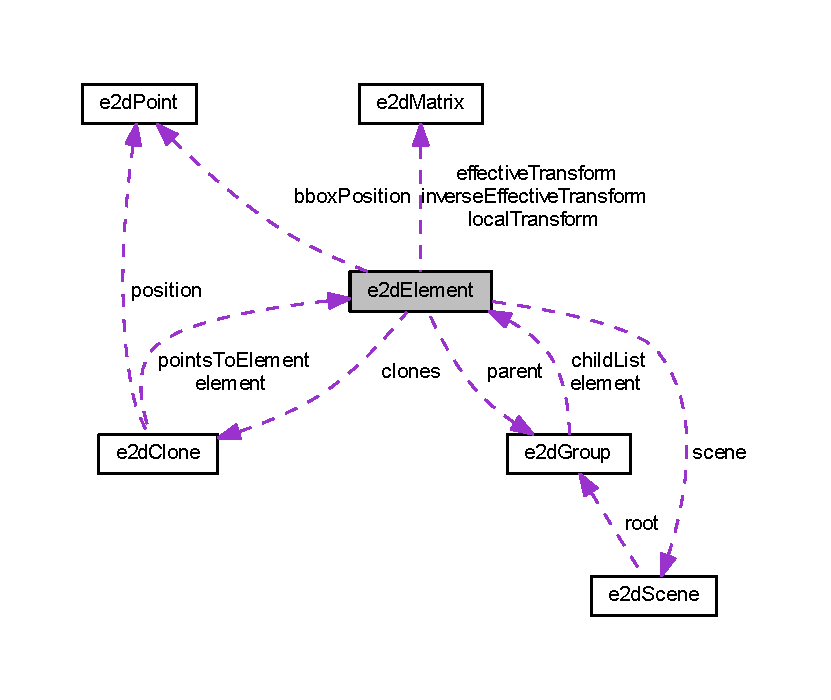
\includegraphics[width=350pt]{structe2dElement__coll__graph}
\end{center}
\end{figure}
\subsection*{Data Fields}
\begin{DoxyCompactItemize}
\item 
\hyperlink{structe2dScene}{e2d\-Scene} $\ast$ \hyperlink{structe2dElement_a0ebd8fae058dd45496c86a2ca317ca9c}{scene}
\item 
\hyperlink{group__e2dElement_ga9bc8cfdec08c7e9069fc707ee456fd38}{e2d\-Element\-Type} \hyperlink{structe2dElement_a7df43d7f6c23b61b843acb56eb3ca19a}{type}
\item 
char $\ast$ \hyperlink{structe2dElement_aecb3b0d045ada529257a2fbf8f829599}{id}
\item 
unsigned int \hyperlink{structe2dElement_a300bb6cf5b184e200523e9bce8346dc4}{unique\-\_\-id}
\item 
\hyperlink{structe2dMatrix}{e2d\-Matrix} \hyperlink{structe2dElement_a52bda732df714953f93c1e6f5f7c7c93}{local\-Transform}
\item 
\hyperlink{structe2dMatrix}{e2d\-Matrix} \hyperlink{structe2dElement_a6c8e26945f09b5157e2111e42f99b879}{effective\-Transform}
\item 
\hyperlink{structe2dMatrix}{e2d\-Matrix} \hyperlink{structe2dElement_a5e6d7341f2dbef1923b0a3fcc13781c6}{inverse\-Effective\-Transform}
\item 
\hyperlink{structe2dGroup}{e2d\-Group} $\ast$ \hyperlink{structe2dElement_a3e62eb2fbf1d6bc6d6fe549096a6cee9}{parent}
\item 
unsigned int \hyperlink{structe2dElement_a836181401227a3ca42da026a8d35e730}{attribute\-Num}
\item 
unsigned int \hyperlink{structe2dElement_a70d94929e3789bf7c019c939b0084985}{attribute\-Alloc}
\item 
char $\ast$$\ast$ \hyperlink{structe2dElement_af9b5d9dbbf270b6f92a3ee66ce1b47ac}{attribute\-Names}
\item 
char $\ast$$\ast$ \hyperlink{structe2dElement_ae8591ff93c366b4d66817a70f2d9f33e}{attribute\-Values}
\item 
float \hyperlink{structe2dElement_a6a1d9b223870deeaec7f5e8b23ca4b22}{bbox\-Width}
\item 
float \hyperlink{structe2dElement_a680d0d4219ac8720005c46b55a9676ae}{bbox\-Height}
\item 
\hyperlink{structe2dPoint}{e2d\-Point} \hyperlink{structe2dElement_ac2c17ce4cba805b594b314a77923cbf5}{bbox\-Position}
\item 
\hyperlink{structe2dClone}{e2d\-Clone} $\ast$$\ast$ \hyperlink{structe2dElement_a4347bc7eb8d31d574115ef75ae074bb7}{clones}
\item 
unsigned int \hyperlink{structe2dElement_ab4c733639f1fdab67f8d25a1439a8b1a}{clones\-Num}
\item 
unsigned int \hyperlink{structe2dElement_a4bdf6d903ed95cd67debbba1ef3dbdae}{clones\-Alloc}
\end{DoxyCompactItemize}


\subsection{Detailed Description}
The \hyperlink{structe2dElement}{e2d\-Element} struct is the base of all elements in the scene. Common scene information such as id, attribute values or transformations are saved in the \hyperlink{structe2dElement}{e2d\-Element} struct. You are not meant to instance this struct by itself. By creating other elements such as \hyperlink{structe2dGroup}{e2d\-Group} or \hyperlink{structe2dImage}{e2d\-Image}, this struct will be automatically allocated in them. This \char`\"{}inheritance\char`\"{} is mimic'd by placing the \hyperlink{structe2dElement}{e2d\-Element} struct as the first element in structs which are meant to be \char`\"{}substructs\char`\"{} of it. 

\subsection{Field Documentation}
\hypertarget{structe2dElement_a70d94929e3789bf7c019c939b0084985}{\index{e2d\-Element@{e2d\-Element}!attribute\-Alloc@{attribute\-Alloc}}
\index{attribute\-Alloc@{attribute\-Alloc}!e2dElement@{e2d\-Element}}
\subsubsection[{attribute\-Alloc}]{\setlength{\rightskip}{0pt plus 5cm}unsigned int {\bf attribute\-Alloc}}}\label{structe2dElement_a70d94929e3789bf7c019c939b0084985}
Allocated size of \hyperlink{structe2dElement_a4347bc7eb8d31d574115ef75ae074bb7}{e2d\-Element\-::clones} \hypertarget{structe2dElement_af9b5d9dbbf270b6f92a3ee66ce1b47ac}{\index{e2d\-Element@{e2d\-Element}!attribute\-Names@{attribute\-Names}}
\index{attribute\-Names@{attribute\-Names}!e2dElement@{e2d\-Element}}
\subsubsection[{attribute\-Names}]{\setlength{\rightskip}{0pt plus 5cm}char$\ast$$\ast$ {\bf attribute\-Names}}}\label{structe2dElement_af9b5d9dbbf270b6f92a3ee66ce1b47ac}
Attribute names array, allocated size given by e2d\-Group\-::attribute\-Alloc. \begin{DoxySeeAlso}{See also}
\hyperlink{group__e2dElement_ga8a9021ff786f5fe61536d1c25ff0e377}{e2d\-Element\-Add\-Attribute()} 
\end{DoxySeeAlso}
\hypertarget{structe2dElement_a836181401227a3ca42da026a8d35e730}{\index{e2d\-Element@{e2d\-Element}!attribute\-Num@{attribute\-Num}}
\index{attribute\-Num@{attribute\-Num}!e2dElement@{e2d\-Element}}
\subsubsection[{attribute\-Num}]{\setlength{\rightskip}{0pt plus 5cm}unsigned int {\bf attribute\-Num}}}\label{structe2dElement_a836181401227a3ca42da026a8d35e730}
Number of attributes in \hyperlink{structe2dElement_af9b5d9dbbf270b6f92a3ee66ce1b47ac}{e2d\-Element\-::attribute\-Names} and \hyperlink{structe2dElement_ae8591ff93c366b4d66817a70f2d9f33e}{e2d\-Element\-::attribute\-Values}. \hypertarget{structe2dElement_ae8591ff93c366b4d66817a70f2d9f33e}{\index{e2d\-Element@{e2d\-Element}!attribute\-Values@{attribute\-Values}}
\index{attribute\-Values@{attribute\-Values}!e2dElement@{e2d\-Element}}
\subsubsection[{attribute\-Values}]{\setlength{\rightskip}{0pt plus 5cm}char$\ast$$\ast$ {\bf attribute\-Values}}}\label{structe2dElement_ae8591ff93c366b4d66817a70f2d9f33e}
Attribute values array, allocated size given by e2d\-Group\-::attribute\-Alloc. \begin{DoxySeeAlso}{See also}
\hyperlink{group__e2dElement_ga8a9021ff786f5fe61536d1c25ff0e377}{e2d\-Element\-Add\-Attribute()} 
\end{DoxySeeAlso}
\hypertarget{structe2dElement_a680d0d4219ac8720005c46b55a9676ae}{\index{e2d\-Element@{e2d\-Element}!bbox\-Height@{bbox\-Height}}
\index{bbox\-Height@{bbox\-Height}!e2dElement@{e2d\-Element}}
\subsubsection[{bbox\-Height}]{\setlength{\rightskip}{0pt plus 5cm}float {\bf bbox\-Height}}}\label{structe2dElement_a680d0d4219ac8720005c46b55a9676ae}
Bounding box height. \begin{DoxySeeAlso}{See also}
\hyperlink{group__e2dElement_ga575c7363927670f1ea8c52b7ea23fcd5}{e2d\-Element\-Calculate\-Bounding\-Box()} 

\hyperlink{group__e2dElement_gab829b280fa22a3509c40425fc84b5061}{e2d\-Element\-Center\-At\-B\-Box()} 
\end{DoxySeeAlso}
\hypertarget{structe2dElement_ac2c17ce4cba805b594b314a77923cbf5}{\index{e2d\-Element@{e2d\-Element}!bbox\-Position@{bbox\-Position}}
\index{bbox\-Position@{bbox\-Position}!e2dElement@{e2d\-Element}}
\subsubsection[{bbox\-Position}]{\setlength{\rightskip}{0pt plus 5cm}{\bf e2d\-Point} {\bf bbox\-Position}}}\label{structe2dElement_ac2c17ce4cba805b594b314a77923cbf5}
Bounding box position. \begin{DoxySeeAlso}{See also}
\hyperlink{group__e2dElement_ga575c7363927670f1ea8c52b7ea23fcd5}{e2d\-Element\-Calculate\-Bounding\-Box()} 

\hyperlink{group__e2dElement_gab829b280fa22a3509c40425fc84b5061}{e2d\-Element\-Center\-At\-B\-Box()} 
\end{DoxySeeAlso}
\hypertarget{structe2dElement_a6a1d9b223870deeaec7f5e8b23ca4b22}{\index{e2d\-Element@{e2d\-Element}!bbox\-Width@{bbox\-Width}}
\index{bbox\-Width@{bbox\-Width}!e2dElement@{e2d\-Element}}
\subsubsection[{bbox\-Width}]{\setlength{\rightskip}{0pt plus 5cm}float {\bf bbox\-Width}}}\label{structe2dElement_a6a1d9b223870deeaec7f5e8b23ca4b22}
Bounding box width. \begin{DoxySeeAlso}{See also}
\hyperlink{group__e2dElement_ga575c7363927670f1ea8c52b7ea23fcd5}{e2d\-Element\-Calculate\-Bounding\-Box()} 

\hyperlink{group__e2dElement_gab829b280fa22a3509c40425fc84b5061}{e2d\-Element\-Center\-At\-B\-Box()} 
\end{DoxySeeAlso}
\hypertarget{structe2dElement_a4347bc7eb8d31d574115ef75ae074bb7}{\index{e2d\-Element@{e2d\-Element}!clones@{clones}}
\index{clones@{clones}!e2dElement@{e2d\-Element}}
\subsubsection[{clones}]{\setlength{\rightskip}{0pt plus 5cm}{\bf e2d\-Clone}$\ast$$\ast$ {\bf clones}}}\label{structe2dElement_a4347bc7eb8d31d574115ef75ae074bb7}
Clones array, allocated size given by \hyperlink{structe2dElement_a4bdf6d903ed95cd67debbba1ef3dbdae}{e2d\-Element\-::clones\-Alloc}. \begin{DoxySeeAlso}{See also}
\hyperlink{group__e2dElement_ga80b7a45c28ec6e95d97b0316358a3290}{e2d\-Element\-Add\-Clone()} 
\end{DoxySeeAlso}
\hypertarget{structe2dElement_a4bdf6d903ed95cd67debbba1ef3dbdae}{\index{e2d\-Element@{e2d\-Element}!clones\-Alloc@{clones\-Alloc}}
\index{clones\-Alloc@{clones\-Alloc}!e2dElement@{e2d\-Element}}
\subsubsection[{clones\-Alloc}]{\setlength{\rightskip}{0pt plus 5cm}unsigned int {\bf clones\-Alloc}}}\label{structe2dElement_a4bdf6d903ed95cd67debbba1ef3dbdae}
Allocated size of \hyperlink{structe2dElement_a4347bc7eb8d31d574115ef75ae074bb7}{e2d\-Element\-::clones} \hypertarget{structe2dElement_ab4c733639f1fdab67f8d25a1439a8b1a}{\index{e2d\-Element@{e2d\-Element}!clones\-Num@{clones\-Num}}
\index{clones\-Num@{clones\-Num}!e2dElement@{e2d\-Element}}
\subsubsection[{clones\-Num}]{\setlength{\rightskip}{0pt plus 5cm}unsigned int {\bf clones\-Num}}}\label{structe2dElement_ab4c733639f1fdab67f8d25a1439a8b1a}
Number of clones in \hyperlink{structe2dElement_a4347bc7eb8d31d574115ef75ae074bb7}{e2d\-Element\-::clones} \hypertarget{structe2dElement_a6c8e26945f09b5157e2111e42f99b879}{\index{e2d\-Element@{e2d\-Element}!effective\-Transform@{effective\-Transform}}
\index{effective\-Transform@{effective\-Transform}!e2dElement@{e2d\-Element}}
\subsubsection[{effective\-Transform}]{\setlength{\rightskip}{0pt plus 5cm}{\bf e2d\-Matrix} {\bf effective\-Transform}}}\label{structe2dElement_a6c8e26945f09b5157e2111e42f99b879}
Actual transform calculated applied here. \begin{DoxySeeAlso}{See also}
\hyperlink{group__e2dScene_ga6981f2448904c96723449cb84ffb4d8a}{e2d\-Scene\-Calculate\-Effective\-Transforms()} 
\end{DoxySeeAlso}
\hypertarget{structe2dElement_aecb3b0d045ada529257a2fbf8f829599}{\index{e2d\-Element@{e2d\-Element}!id@{id}}
\index{id@{id}!e2dElement@{e2d\-Element}}
\subsubsection[{id}]{\setlength{\rightskip}{0pt plus 5cm}char$\ast$ {\bf id}}}\label{structe2dElement_aecb3b0d045ada529257a2fbf8f829599}
I\-D taken from S\-V\-G \hypertarget{structe2dElement_a5e6d7341f2dbef1923b0a3fcc13781c6}{\index{e2d\-Element@{e2d\-Element}!inverse\-Effective\-Transform@{inverse\-Effective\-Transform}}
\index{inverse\-Effective\-Transform@{inverse\-Effective\-Transform}!e2dElement@{e2d\-Element}}
\subsubsection[{inverse\-Effective\-Transform}]{\setlength{\rightskip}{0pt plus 5cm}{\bf e2d\-Matrix} {\bf inverse\-Effective\-Transform}}}\label{structe2dElement_a5e6d7341f2dbef1923b0a3fcc13781c6}
Useful for point transformations.

\begin{DoxySeeAlso}{See also}
\hyperlink{group__e2dElement_ga9e3e35d789556a05a4bd439b8cae01f2}{e2d\-Element\-Get\-Local\-Position()} 

\hyperlink{group__e2dElement_ga542b7ae5370bd59e118ed656588d3029}{e2d\-Element\-Get\-World\-Position()} 

\hyperlink{group__e2dElement_gaa00ae93ed9fb9d27db2513e3f05a0827}{e2d\-Element\-Get\-Relative\-Position()} 

\hyperlink{group__e2dElement_gae6b6f57ac5505ef9181289197d419536}{e2d\-Element\-Get\-Relative\-Point()} 
\end{DoxySeeAlso}
\hypertarget{structe2dElement_a52bda732df714953f93c1e6f5f7c7c93}{\index{e2d\-Element@{e2d\-Element}!local\-Transform@{local\-Transform}}
\index{local\-Transform@{local\-Transform}!e2dElement@{e2d\-Element}}
\subsubsection[{local\-Transform}]{\setlength{\rightskip}{0pt plus 5cm}{\bf e2d\-Matrix} {\bf local\-Transform}}}\label{structe2dElement_a52bda732df714953f93c1e6f5f7c7c93}
Local\-Transform taken from S\-V\-G \hypertarget{structe2dElement_a3e62eb2fbf1d6bc6d6fe549096a6cee9}{\index{e2d\-Element@{e2d\-Element}!parent@{parent}}
\index{parent@{parent}!e2dElement@{e2d\-Element}}
\subsubsection[{parent}]{\setlength{\rightskip}{0pt plus 5cm}{\bf e2d\-Group}$\ast$ {\bf parent}}}\label{structe2dElement_a3e62eb2fbf1d6bc6d6fe549096a6cee9}
parent of the element in the scene tree. \hypertarget{structe2dElement_a0ebd8fae058dd45496c86a2ca317ca9c}{\index{e2d\-Element@{e2d\-Element}!scene@{scene}}
\index{scene@{scene}!e2dElement@{e2d\-Element}}
\subsubsection[{scene}]{\setlength{\rightskip}{0pt plus 5cm}{\bf e2d\-Scene}$\ast$ {\bf scene}}}\label{structe2dElement_a0ebd8fae058dd45496c86a2ca317ca9c}
Belongs to this scene \hypertarget{structe2dElement_a7df43d7f6c23b61b843acb56eb3ca19a}{\index{e2d\-Element@{e2d\-Element}!type@{type}}
\index{type@{type}!e2dElement@{e2d\-Element}}
\subsubsection[{type}]{\setlength{\rightskip}{0pt plus 5cm}{\bf e2d\-Element\-Type} {\bf type}}}\label{structe2dElement_a7df43d7f6c23b61b843acb56eb3ca19a}
Used for reflection \hypertarget{structe2dElement_a300bb6cf5b184e200523e9bce8346dc4}{\index{e2d\-Element@{e2d\-Element}!unique\-\_\-id@{unique\-\_\-id}}
\index{unique\-\_\-id@{unique\-\_\-id}!e2dElement@{e2d\-Element}}
\subsubsection[{unique\-\_\-id}]{\setlength{\rightskip}{0pt plus 5cm}unsigned int {\bf unique\-\_\-id}}}\label{structe2dElement_a300bb6cf5b184e200523e9bce8346dc4}
unique id for this execution. (static int in \hyperlink{group__e2dGroup_gafa3f224a6509fbff5063dc910d4e3f1e}{e2d\-Group\-Init()} ) 

The documentation for this struct was generated from the following file\-:\begin{DoxyCompactItemize}
\item 
\hyperlink{e2dElement_8h}{e2d\-Element.\-h}\end{DoxyCompactItemize}

\hypertarget{structe2dGroup}{\section{e2d\-Group Struct Reference}
\label{structe2dGroup}\index{e2d\-Group@{e2d\-Group}}
}


The \hyperlink{structe2dGroup}{e2d\-Group} struct is used to group elements in the scene. This struct is created from the \char`\"{}g\char`\"{} element in S\-V\-G. It \char`\"{}inherits\char`\"{} from \hyperlink{structe2dElement}{e2d\-Element} by placing it as the first element in the struct, if you typecast e2d\-Group$\ast$ into e2d\-Element$\ast$, it will work thus mimicing inheritance in e.\-g. C++.  




{\ttfamily \#include $<$e2d\-Group.\-h$>$}



Collaboration diagram for e2d\-Group\-:\nopagebreak
\begin{figure}[H]
\begin{center}
\leavevmode
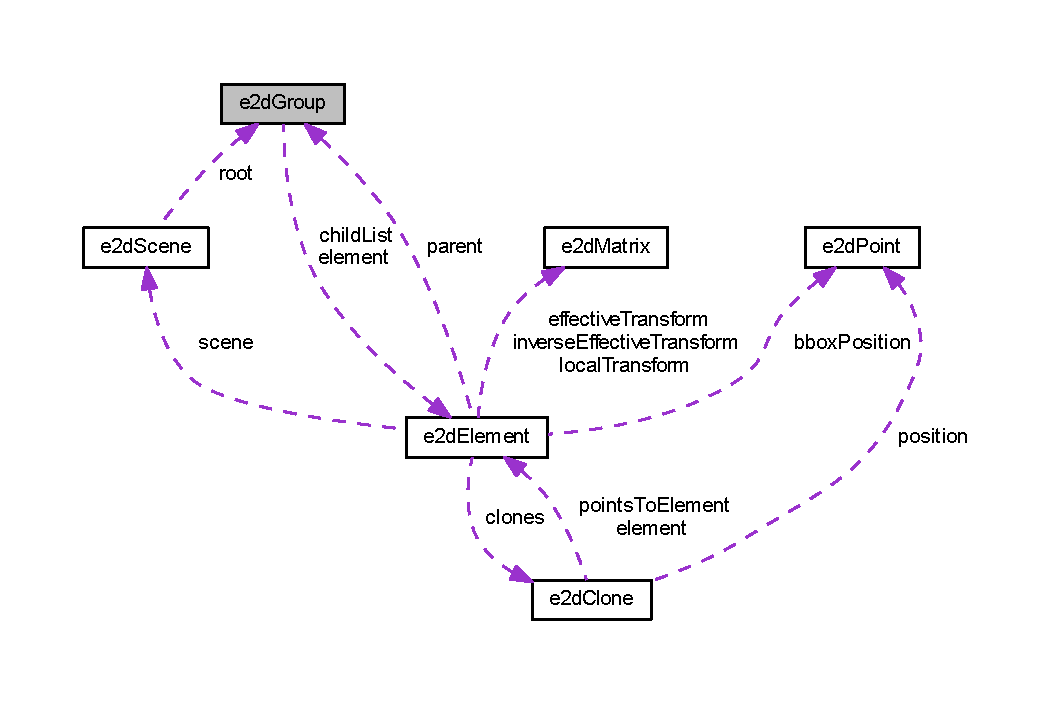
\includegraphics[width=350pt]{structe2dGroup__coll__graph}
\end{center}
\end{figure}
\subsection*{Data Fields}
\begin{DoxyCompactItemize}
\item 
\hyperlink{structe2dElement}{e2d\-Element} \hyperlink{structe2dGroup_a55bc7a3a0af41fba9e5b91f390c5928c}{element}
\item 
unsigned int \hyperlink{structe2dGroup_a0af3697c2c9df6ed0ddd340cded35d65}{child\-Num}
\item 
\hyperlink{structe2dElement}{e2d\-Element} $\ast$$\ast$ \hyperlink{structe2dGroup_a55f6dde874716dc99dcd270fc0999a01}{child\-List}
\item 
unsigned int \hyperlink{structe2dGroup_a9c89d7cf35b835ef1917855c78a79cc5}{child\-List\-Alloc}
\end{DoxyCompactItemize}


\subsection{Detailed Description}
The \hyperlink{structe2dGroup}{e2d\-Group} struct is used to group elements in the scene. This struct is created from the \char`\"{}g\char`\"{} element in S\-V\-G. It \char`\"{}inherits\char`\"{} from \hyperlink{structe2dElement}{e2d\-Element} by placing it as the first element in the struct, if you typecast e2d\-Group$\ast$ into e2d\-Element$\ast$, it will work thus mimicing inheritance in e.\-g. C++. 

\subsection{Field Documentation}
\hypertarget{structe2dGroup_a55f6dde874716dc99dcd270fc0999a01}{\index{e2d\-Group@{e2d\-Group}!child\-List@{child\-List}}
\index{child\-List@{child\-List}!e2dGroup@{e2d\-Group}}
\subsubsection[{child\-List}]{\setlength{\rightskip}{0pt plus 5cm}{\bf e2d\-Element}$\ast$$\ast$ {\bf child\-List}}}\label{structe2dGroup_a55f6dde874716dc99dcd270fc0999a01}
Child list array, allocated size given by \hyperlink{structe2dGroup_a9c89d7cf35b835ef1917855c78a79cc5}{e2d\-Group\-::child\-List\-Alloc}. \begin{DoxySeeAlso}{See also}
\hyperlink{group__e2dGroup_ga6ae76730f78ad731621e9286a3980b8a}{e2d\-Group\-Add\-Child()} 
\end{DoxySeeAlso}
\hypertarget{structe2dGroup_a9c89d7cf35b835ef1917855c78a79cc5}{\index{e2d\-Group@{e2d\-Group}!child\-List\-Alloc@{child\-List\-Alloc}}
\index{child\-List\-Alloc@{child\-List\-Alloc}!e2dGroup@{e2d\-Group}}
\subsubsection[{child\-List\-Alloc}]{\setlength{\rightskip}{0pt plus 5cm}unsigned int {\bf child\-List\-Alloc}}}\label{structe2dGroup_a9c89d7cf35b835ef1917855c78a79cc5}
Allocated size of \hyperlink{structe2dGroup_a55f6dde874716dc99dcd270fc0999a01}{e2d\-Group\-::child\-List} \hypertarget{structe2dGroup_a0af3697c2c9df6ed0ddd340cded35d65}{\index{e2d\-Group@{e2d\-Group}!child\-Num@{child\-Num}}
\index{child\-Num@{child\-Num}!e2dGroup@{e2d\-Group}}
\subsubsection[{child\-Num}]{\setlength{\rightskip}{0pt plus 5cm}unsigned int {\bf child\-Num}}}\label{structe2dGroup_a0af3697c2c9df6ed0ddd340cded35d65}
Number of children in \hyperlink{structe2dGroup_a55f6dde874716dc99dcd270fc0999a01}{e2d\-Group\-::child\-List} Array \hypertarget{structe2dGroup_a55bc7a3a0af41fba9e5b91f390c5928c}{\index{e2d\-Group@{e2d\-Group}!element@{element}}
\index{element@{element}!e2dGroup@{e2d\-Group}}
\subsubsection[{element}]{\setlength{\rightskip}{0pt plus 5cm}{\bf e2d\-Element} {\bf element}}}\label{structe2dGroup_a55bc7a3a0af41fba9e5b91f390c5928c}
\hyperlink{structe2dGroup}{e2d\-Group} inherits from \hyperlink{structe2dElement}{e2d\-Element}. Typecasting e2d\-Group$\ast$ to e2d\-Element$\ast$ will work. 

The documentation for this struct was generated from the following file\-:\begin{DoxyCompactItemize}
\item 
\hyperlink{e2dGroup_8h}{e2d\-Group.\-h}\end{DoxyCompactItemize}

\hypertarget{structe2dGroupIterator}{\section{e2d\-Group\-Iterator Struct Reference}
\label{structe2dGroupIterator}\index{e2d\-Group\-Iterator@{e2d\-Group\-Iterator}}
}


An iterator for the children of \hyperlink{structe2dGroup}{e2d\-Group}.  




{\ttfamily \#include $<$e2d\-Group.\-h$>$}



Collaboration diagram for e2d\-Group\-Iterator\-:\nopagebreak
\begin{figure}[H]
\begin{center}
\leavevmode
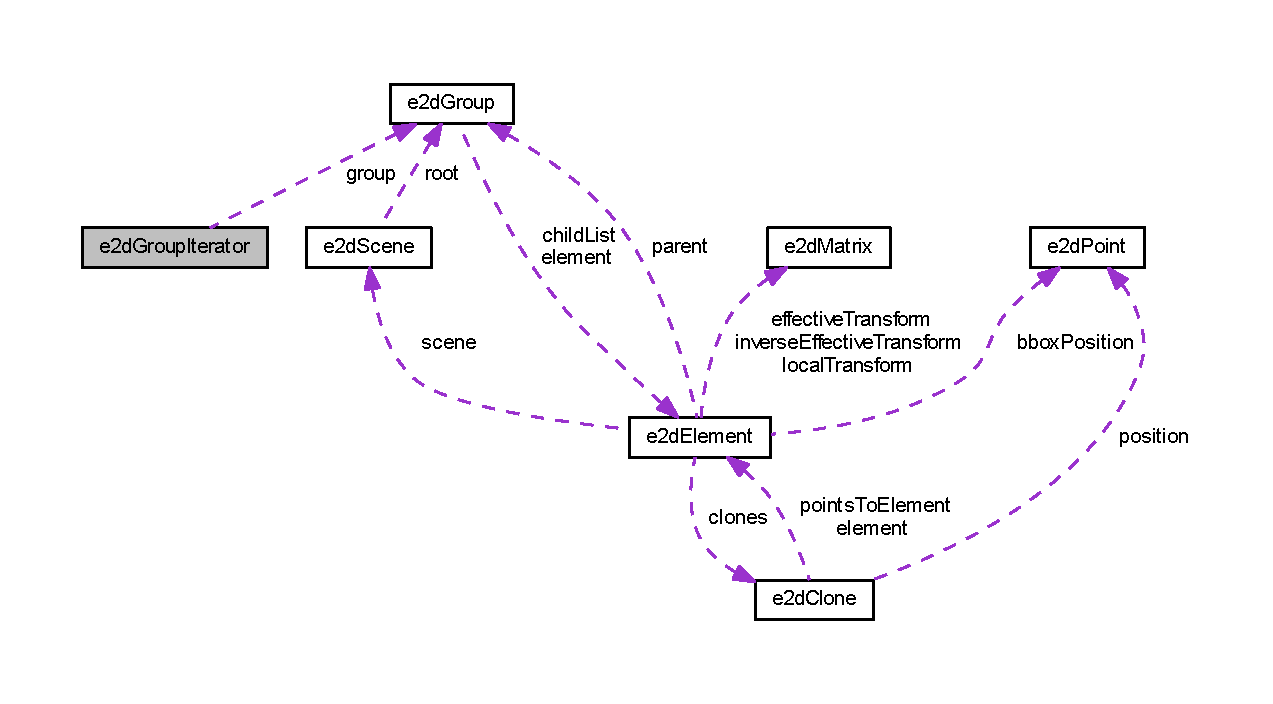
\includegraphics[width=350pt]{structe2dGroupIterator__coll__graph}
\end{center}
\end{figure}
\subsection*{Data Fields}
\begin{DoxyCompactItemize}
\item 
\hyperlink{structe2dGroup}{e2d\-Group} $\ast$ \hyperlink{structe2dGroupIterator_a13e9c2162587f7af49d2ceb78c380444}{group}
\item 
unsigned int \hyperlink{structe2dGroupIterator_a932f59c8e81a171eb21af8d204d1c13d}{current\-Index}
\end{DoxyCompactItemize}


\subsection{Detailed Description}
An iterator for the children of \hyperlink{structe2dGroup}{e2d\-Group}. 

\subsection{Field Documentation}
\hypertarget{structe2dGroupIterator_a932f59c8e81a171eb21af8d204d1c13d}{\index{e2d\-Group\-Iterator@{e2d\-Group\-Iterator}!current\-Index@{current\-Index}}
\index{current\-Index@{current\-Index}!e2dGroupIterator@{e2d\-Group\-Iterator}}
\subsubsection[{current\-Index}]{\setlength{\rightskip}{0pt plus 5cm}unsigned int {\bf current\-Index}}}\label{structe2dGroupIterator_a932f59c8e81a171eb21af8d204d1c13d}
Current index in \hyperlink{structe2dGroup_a55f6dde874716dc99dcd270fc0999a01}{e2d\-Group\-::child\-List}. \hypertarget{structe2dGroupIterator_a13e9c2162587f7af49d2ceb78c380444}{\index{e2d\-Group\-Iterator@{e2d\-Group\-Iterator}!group@{group}}
\index{group@{group}!e2dGroupIterator@{e2d\-Group\-Iterator}}
\subsubsection[{group}]{\setlength{\rightskip}{0pt plus 5cm}{\bf e2d\-Group}$\ast$ {\bf group}}}\label{structe2dGroupIterator_a13e9c2162587f7af49d2ceb78c380444}
This iterator is working on this group. 

The documentation for this struct was generated from the following file\-:\begin{DoxyCompactItemize}
\item 
\hyperlink{e2dGroup_8h}{e2d\-Group.\-h}\end{DoxyCompactItemize}

\hypertarget{structe2dImage}{\section{e2d\-Image Struct Reference}
\label{structe2dImage}\index{e2d\-Image@{e2d\-Image}}
}


The \hyperlink{structe2dImage}{e2d\-Image} struct is used for holding the paths to images and their size and position. The struct is composed directly from the contents of the S\-V\-G image element. It \char`\"{}inherits\char`\"{} from \hyperlink{structe2dElement}{e2d\-Element} by placing it as the first element in the struct, if you typecast e2d\-Image$\ast$ into e2d\-Element$\ast$, it will work thus mimicing inheritance in e.\-g. C++.  




{\ttfamily \#include $<$e2d\-Image.\-h$>$}



Collaboration diagram for e2d\-Image\-:\nopagebreak
\begin{figure}[H]
\begin{center}
\leavevmode
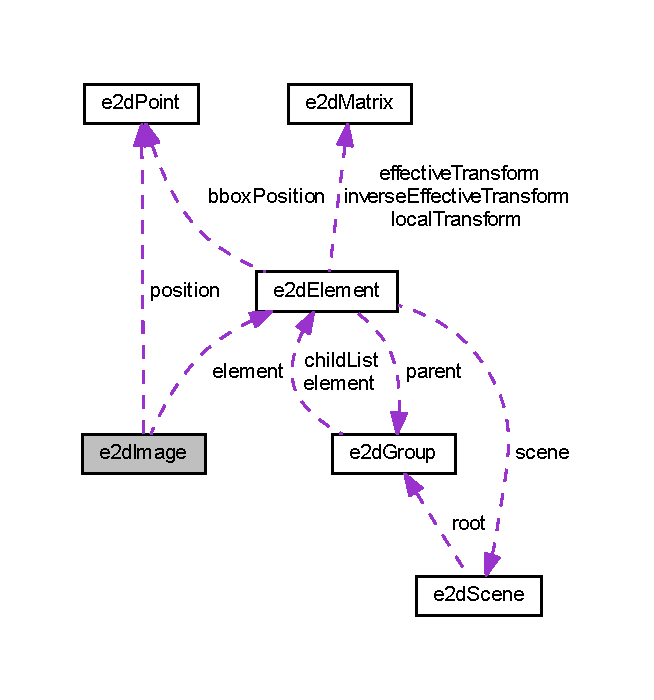
\includegraphics[width=350pt]{structe2dImage__coll__graph}
\end{center}
\end{figure}
\subsection*{Data Fields}
\begin{DoxyCompactItemize}
\item 
\hyperlink{structe2dElement}{e2d\-Element} \hyperlink{structe2dImage_a55bc7a3a0af41fba9e5b91f390c5928c}{element}
\item 
\hyperlink{structe2dPoint}{e2d\-Point} \hyperlink{structe2dImage_afa8983f25fd6aa6aca18feb07d8d2249}{position}
\item 
float \hyperlink{structe2dImage_ae426f00e82704fa09578f5446e22d915}{width}
\item 
float \hyperlink{structe2dImage_a48083b65ac9a863566dc3e3fff09a5b4}{height}
\item 
char $\ast$ \hyperlink{structe2dImage_afb14ab23ba86115c3b01ad4122943f89}{image\-Path}
\end{DoxyCompactItemize}


\subsection{Detailed Description}
The \hyperlink{structe2dImage}{e2d\-Image} struct is used for holding the paths to images and their size and position. The struct is composed directly from the contents of the S\-V\-G image element. It \char`\"{}inherits\char`\"{} from \hyperlink{structe2dElement}{e2d\-Element} by placing it as the first element in the struct, if you typecast e2d\-Image$\ast$ into e2d\-Element$\ast$, it will work thus mimicing inheritance in e.\-g. C++. 

\subsection{Field Documentation}
\hypertarget{structe2dImage_a55bc7a3a0af41fba9e5b91f390c5928c}{\index{e2d\-Image@{e2d\-Image}!element@{element}}
\index{element@{element}!e2dImage@{e2d\-Image}}
\subsubsection[{element}]{\setlength{\rightskip}{0pt plus 5cm}{\bf e2d\-Element} {\bf element}}}\label{structe2dImage_a55bc7a3a0af41fba9e5b91f390c5928c}
\hyperlink{structe2dImage}{e2d\-Image} inherits from \hyperlink{structe2dElement}{e2d\-Element}. Typecasting e2d\-Image$\ast$ to e2d\-Element$\ast$ will work. \hypertarget{structe2dImage_a48083b65ac9a863566dc3e3fff09a5b4}{\index{e2d\-Image@{e2d\-Image}!height@{height}}
\index{height@{height}!e2dImage@{e2d\-Image}}
\subsubsection[{height}]{\setlength{\rightskip}{0pt plus 5cm}float {\bf height}}}\label{structe2dImage_a48083b65ac9a863566dc3e3fff09a5b4}
Height of the image, may be -\/1 if not defined in the S\-V\-G \hypertarget{structe2dImage_afb14ab23ba86115c3b01ad4122943f89}{\index{e2d\-Image@{e2d\-Image}!image\-Path@{image\-Path}}
\index{image\-Path@{image\-Path}!e2dImage@{e2d\-Image}}
\subsubsection[{image\-Path}]{\setlength{\rightskip}{0pt plus 5cm}char$\ast$ {\bf image\-Path}}}\label{structe2dImage_afb14ab23ba86115c3b01ad4122943f89}
Path to the image. This is taken directly from the S\-V\-G, so if you are getting a local path for example, you need to fix it on the S\-V\-G. \hypertarget{structe2dImage_afa8983f25fd6aa6aca18feb07d8d2249}{\index{e2d\-Image@{e2d\-Image}!position@{position}}
\index{position@{position}!e2dImage@{e2d\-Image}}
\subsubsection[{position}]{\setlength{\rightskip}{0pt plus 5cm}{\bf e2d\-Point} {\bf position}}}\label{structe2dImage_afa8983f25fd6aa6aca18feb07d8d2249}
Position of the image. Note that it is after applying the transformation present in \hyperlink{structe2dElement_a52bda732df714953f93c1e6f5f7c7c93}{e2d\-Element\-::local\-Transform}. \hypertarget{structe2dImage_ae426f00e82704fa09578f5446e22d915}{\index{e2d\-Image@{e2d\-Image}!width@{width}}
\index{width@{width}!e2dImage@{e2d\-Image}}
\subsubsection[{width}]{\setlength{\rightskip}{0pt plus 5cm}float {\bf width}}}\label{structe2dImage_ae426f00e82704fa09578f5446e22d915}
Width of the image, may be -\/1 if not defined in the S\-V\-G 

The documentation for this struct was generated from the following file\-:\begin{DoxyCompactItemize}
\item 
\hyperlink{e2dImage_8h}{e2d\-Image.\-h}\end{DoxyCompactItemize}

\hypertarget{structe2dMatrix}{\section{e2d\-Matrix Struct Reference}
\label{structe2dMatrix}\index{e2d\-Matrix@{e2d\-Matrix}}
}


The \hyperlink{structe2dMatrix}{e2d\-Matrix} struct contains the implementation of a 3x3 matrix which is row major. See \href{http://en.wikipedia.org/wiki/Row-major_order}{\tt http\-://en.\-wikipedia.\-org/wiki/\-Row-\/major\-\_\-order} if you have doubts.  




{\ttfamily \#include $<$e2d\-Matrix.\-h$>$}

\subsection*{Data Fields}
\begin{DoxyCompactItemize}
\item 
float \hyperlink{structe2dMatrix_ac06a92ccf2617d904678c51c6cf5a9bb}{vals} \mbox{[}3\mbox{]}\mbox{[}3\mbox{]}
\end{DoxyCompactItemize}


\subsection{Detailed Description}
The \hyperlink{structe2dMatrix}{e2d\-Matrix} struct contains the implementation of a 3x3 matrix which is row major. See \href{http://en.wikipedia.org/wiki/Row-major_order}{\tt http\-://en.\-wikipedia.\-org/wiki/\-Row-\/major\-\_\-order} if you have doubts. 

\subsection{Field Documentation}
\hypertarget{structe2dMatrix_ac06a92ccf2617d904678c51c6cf5a9bb}{\index{e2d\-Matrix@{e2d\-Matrix}!vals@{vals}}
\index{vals@{vals}!e2dMatrix@{e2d\-Matrix}}
\subsubsection[{vals}]{\setlength{\rightskip}{0pt plus 5cm}float {\bf vals}\mbox{[}3\mbox{]}\mbox{[}3\mbox{]}}}\label{structe2dMatrix_ac06a92ccf2617d904678c51c6cf5a9bb}
Row major 3x3 matrix array 

The documentation for this struct was generated from the following file\-:\begin{DoxyCompactItemize}
\item 
\hyperlink{e2dMatrix_8h}{e2d\-Matrix.\-h}\end{DoxyCompactItemize}

\hypertarget{structe2dPath}{\section{e2d\-Path Struct Reference}
\label{structe2dPath}\index{e2d\-Path@{e2d\-Path}}
}


The \hyperlink{structe2dPath}{e2d\-Path} struct is used for holding the information of path. The struct is composed directly from the contents of the S\-V\-G path element. It \char`\"{}inherits\char`\"{} from \hyperlink{structe2dElement}{e2d\-Element} by placing it as the first element in the struct, if you typecast e2d\-Path$\ast$ into e2d\-Element$\ast$, it will work thus mimicing inheritance in e.\-g. C++.  




{\ttfamily \#include $<$e2d\-Path.\-h$>$}



Collaboration diagram for e2d\-Path\-:\nopagebreak
\begin{figure}[H]
\begin{center}
\leavevmode
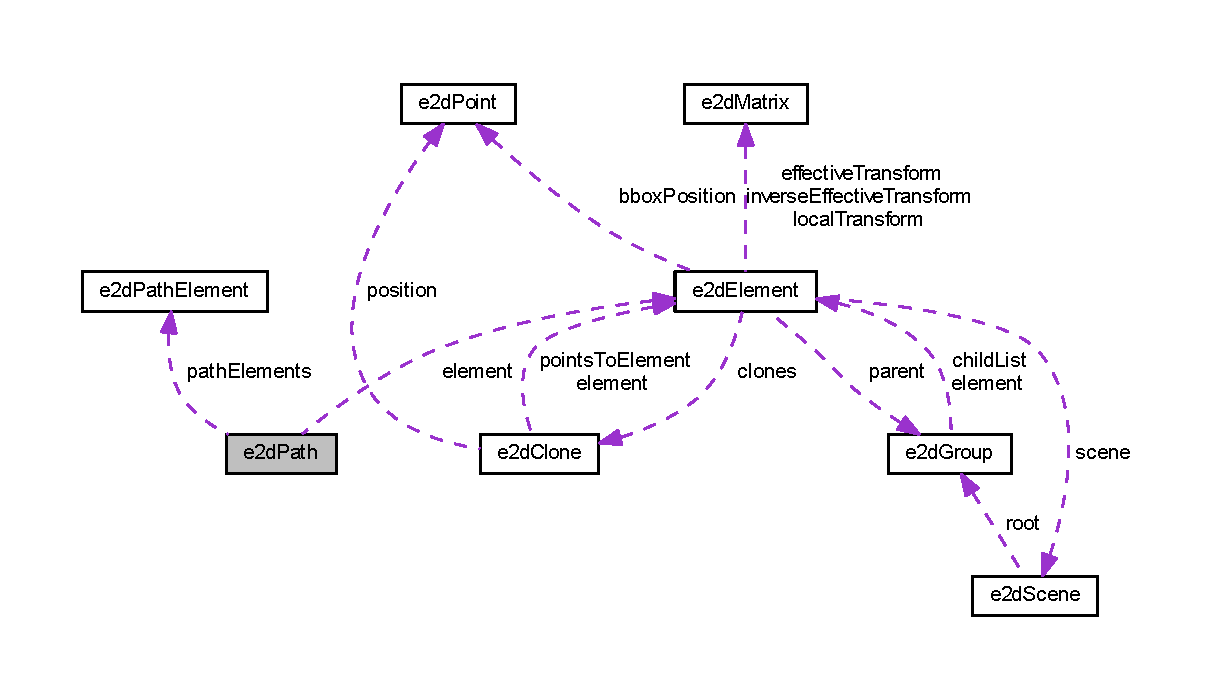
\includegraphics[width=350pt]{structe2dPath__coll__graph}
\end{center}
\end{figure}
\subsection*{Data Fields}
\begin{DoxyCompactItemize}
\item 
\hyperlink{structe2dElement}{e2d\-Element} \hyperlink{structe2dPath_a55bc7a3a0af41fba9e5b91f390c5928c}{element}
\item 
unsigned int \hyperlink{structe2dPath_a225f71916c061d0c977a1e5fae371a99}{path\-Elements\-Num}
\item 
\hyperlink{structe2dPathElement}{e2d\-Path\-Element} $\ast$$\ast$ \hyperlink{structe2dPath_ac0c8a45ff4f8d02e557fb33887743439}{path\-Elements}
\item 
unsigned int \hyperlink{structe2dPath_a0922122c6ccf006fad850c6b30ae5328}{path\-Elements\-Alloc}
\end{DoxyCompactItemize}


\subsection{Detailed Description}
The \hyperlink{structe2dPath}{e2d\-Path} struct is used for holding the information of path. The struct is composed directly from the contents of the S\-V\-G path element. It \char`\"{}inherits\char`\"{} from \hyperlink{structe2dElement}{e2d\-Element} by placing it as the first element in the struct, if you typecast e2d\-Path$\ast$ into e2d\-Element$\ast$, it will work thus mimicing inheritance in e.\-g. C++. 

\subsection{Field Documentation}
\hypertarget{structe2dPath_a55bc7a3a0af41fba9e5b91f390c5928c}{\index{e2d\-Path@{e2d\-Path}!element@{element}}
\index{element@{element}!e2dPath@{e2d\-Path}}
\subsubsection[{element}]{\setlength{\rightskip}{0pt plus 5cm}{\bf e2d\-Element} {\bf element}}}\label{structe2dPath_a55bc7a3a0af41fba9e5b91f390c5928c}
\hyperlink{structe2dPath}{e2d\-Path} inherits from \hyperlink{structe2dElement}{e2d\-Element}. Typecasting e2d\-Path$\ast$ to e2d\-Element$\ast$ will work. \hypertarget{structe2dPath_ac0c8a45ff4f8d02e557fb33887743439}{\index{e2d\-Path@{e2d\-Path}!path\-Elements@{path\-Elements}}
\index{path\-Elements@{path\-Elements}!e2dPath@{e2d\-Path}}
\subsubsection[{path\-Elements}]{\setlength{\rightskip}{0pt plus 5cm}{\bf e2d\-Path\-Element}$\ast$$\ast$ {\bf path\-Elements}}}\label{structe2dPath_ac0c8a45ff4f8d02e557fb33887743439}
Array containing the path elements \hypertarget{structe2dPath_a0922122c6ccf006fad850c6b30ae5328}{\index{e2d\-Path@{e2d\-Path}!path\-Elements\-Alloc@{path\-Elements\-Alloc}}
\index{path\-Elements\-Alloc@{path\-Elements\-Alloc}!e2dPath@{e2d\-Path}}
\subsubsection[{path\-Elements\-Alloc}]{\setlength{\rightskip}{0pt plus 5cm}unsigned int {\bf path\-Elements\-Alloc}}}\label{structe2dPath_a0922122c6ccf006fad850c6b30ae5328}
Currently allocated memory in the \hyperlink{structe2dPath_ac0c8a45ff4f8d02e557fb33887743439}{e2d\-Path\-::path\-Elements} \hypertarget{structe2dPath_a225f71916c061d0c977a1e5fae371a99}{\index{e2d\-Path@{e2d\-Path}!path\-Elements\-Num@{path\-Elements\-Num}}
\index{path\-Elements\-Num@{path\-Elements\-Num}!e2dPath@{e2d\-Path}}
\subsubsection[{path\-Elements\-Num}]{\setlength{\rightskip}{0pt plus 5cm}unsigned int {\bf path\-Elements\-Num}}}\label{structe2dPath_a225f71916c061d0c977a1e5fae371a99}
Number of elements in \hyperlink{structe2dPath_ac0c8a45ff4f8d02e557fb33887743439}{e2d\-Path\-::path\-Elements} Array 

The documentation for this struct was generated from the following file\-:\begin{DoxyCompactItemize}
\item 
\hyperlink{e2dPath_8h}{e2d\-Path.\-h}\end{DoxyCompactItemize}

\hypertarget{structe2dPathCurve}{\section{e2d\-Path\-Curve Struct Reference}
\label{structe2dPathCurve}\index{e2d\-Path\-Curve@{e2d\-Path\-Curve}}
}


Collaboration diagram for e2d\-Path\-Curve\-:
\nopagebreak
\begin{figure}[H]
\begin{center}
\leavevmode
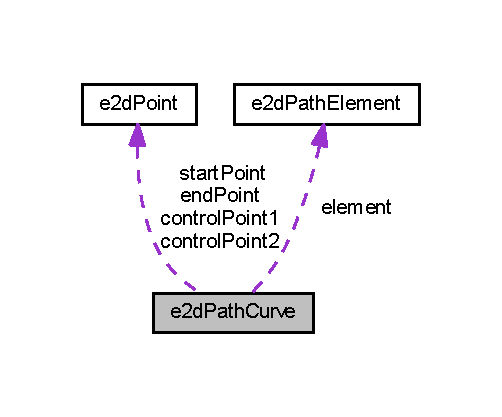
\includegraphics[width=241pt]{structe2dPathCurve__coll__graph}
\end{center}
\end{figure}
\subsection*{Data Fields}
\begin{DoxyCompactItemize}
\item 
\hypertarget{structe2dPathCurve_a88e514266530010a1a3b08198b3cc763}{\hyperlink{structe2dPathElement}{e2d\-Path\-Element} {\bfseries element}}\label{structe2dPathCurve_a88e514266530010a1a3b08198b3cc763}

\item 
\hypertarget{structe2dPathCurve_a96868a222a14861eb6e64214328c6159}{\hyperlink{structe2dPoint}{e2d\-Point} {\bfseries start\-Point}}\label{structe2dPathCurve_a96868a222a14861eb6e64214328c6159}

\item 
\hypertarget{structe2dPathCurve_a5fe58a06185a33704c2cc77c8a58fb0d}{\hyperlink{structe2dPoint}{e2d\-Point} {\bfseries control\-Point1}}\label{structe2dPathCurve_a5fe58a06185a33704c2cc77c8a58fb0d}

\item 
\hypertarget{structe2dPathCurve_a929324aa1e3527d71e312e5f80cb24db}{\hyperlink{structe2dPoint}{e2d\-Point} {\bfseries control\-Point2}}\label{structe2dPathCurve_a929324aa1e3527d71e312e5f80cb24db}

\item 
\hypertarget{structe2dPathCurve_a0ae59a21d141722d36c0ebc740587f9d}{\hyperlink{structe2dPoint}{e2d\-Point} {\bfseries end\-Point}}\label{structe2dPathCurve_a0ae59a21d141722d36c0ebc740587f9d}

\end{DoxyCompactItemize}


The documentation for this struct was generated from the following file\-:\begin{DoxyCompactItemize}
\item 
e2d\-Path.\-h\end{DoxyCompactItemize}

\hypertarget{structe2dPathElement}{\section{e2d\-Path\-Element Struct Reference}
\label{structe2dPathElement}\index{e2d\-Path\-Element@{e2d\-Path\-Element}}
}
\subsection*{Data Fields}
\begin{DoxyCompactItemize}
\item 
\hypertarget{structe2dPathElement_acb2ed01d1856b82777314d8eb8f66b01}{e2d\-Path\-Element\-Type {\bfseries type}}\label{structe2dPathElement_acb2ed01d1856b82777314d8eb8f66b01}

\item 
\hypertarget{structe2dPathElement_a88af317c0c6d0deb1aacb6cc1acd441d}{e2d\-Path\-Control {\bfseries control\-Type}}\label{structe2dPathElement_a88af317c0c6d0deb1aacb6cc1acd441d}

\end{DoxyCompactItemize}


The documentation for this struct was generated from the following file\-:\begin{DoxyCompactItemize}
\item 
e2d\-Path.\-h\end{DoxyCompactItemize}

\hypertarget{structe2dPathElementIterator}{\section{e2d\-Path\-Element\-Iterator Struct Reference}
\label{structe2dPathElementIterator}\index{e2d\-Path\-Element\-Iterator@{e2d\-Path\-Element\-Iterator}}
}


Collaboration diagram for e2d\-Path\-Element\-Iterator\-:
\nopagebreak
\begin{figure}[H]
\begin{center}
\leavevmode
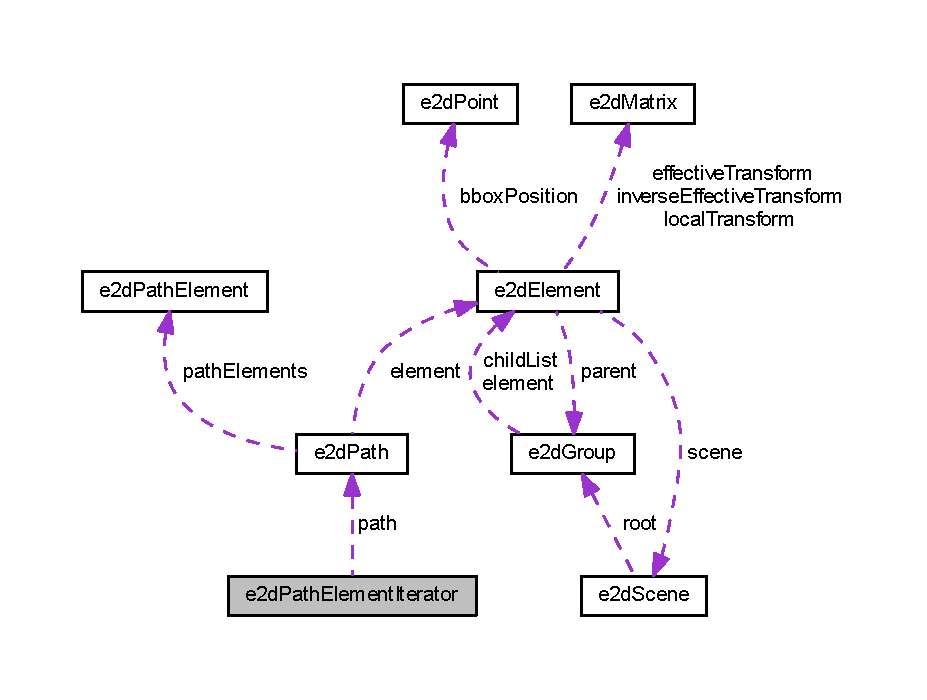
\includegraphics[width=350pt]{structe2dPathElementIterator__coll__graph}
\end{center}
\end{figure}
\subsection*{Data Fields}
\begin{DoxyCompactItemize}
\item 
\hypertarget{structe2dPathElementIterator_a318773d3a24970f193ecb5e2fcdce1a7}{\hyperlink{structe2dPath}{e2d\-Path} $\ast$ {\bfseries path}}\label{structe2dPathElementIterator_a318773d3a24970f193ecb5e2fcdce1a7}

\item 
\hypertarget{structe2dPathElementIterator_a932f59c8e81a171eb21af8d204d1c13d}{unsigned int {\bfseries current\-Index}}\label{structe2dPathElementIterator_a932f59c8e81a171eb21af8d204d1c13d}

\end{DoxyCompactItemize}


The documentation for this struct was generated from the following file\-:\begin{DoxyCompactItemize}
\item 
e2d\-Path.\-h\end{DoxyCompactItemize}

\hypertarget{structe2dPathPoint}{\section{e2d\-Path\-Point Struct Reference}
\label{structe2dPathPoint}\index{e2d\-Path\-Point@{e2d\-Path\-Point}}
}


This struct represents a point in the path. It \char`\"{}inherits\char`\"{} from \hyperlink{structe2dPathElement}{e2d\-Path\-Element} by placing it as the first element in the struct, if you typecast e2d\-Path\-Point$\ast$ into e2d\-Path\-Element$\ast$, it will work thus mimicing inheritance in e.\-g. C++.  




{\ttfamily \#include $<$e2d\-Path.\-h$>$}



Collaboration diagram for e2d\-Path\-Point\-:\nopagebreak
\begin{figure}[H]
\begin{center}
\leavevmode
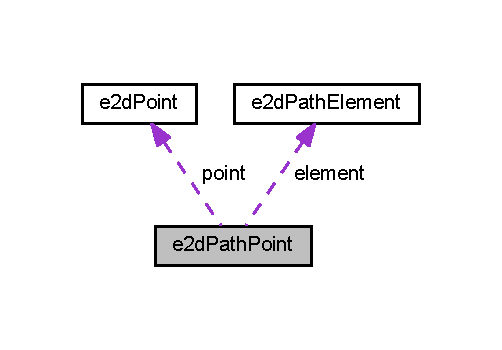
\includegraphics[width=241pt]{structe2dPathPoint__coll__graph}
\end{center}
\end{figure}
\subsection*{Data Fields}
\begin{DoxyCompactItemize}
\item 
\hyperlink{structe2dPathElement}{e2d\-Path\-Element} \hyperlink{structe2dPathPoint_a88e514266530010a1a3b08198b3cc763}{element}
\item 
\hyperlink{structe2dPoint}{e2d\-Point} \hyperlink{structe2dPathPoint_afff60c971a4d4728af80b4753d30c5bf}{point}
\end{DoxyCompactItemize}


\subsection{Detailed Description}
This struct represents a point in the path. It \char`\"{}inherits\char`\"{} from \hyperlink{structe2dPathElement}{e2d\-Path\-Element} by placing it as the first element in the struct, if you typecast e2d\-Path\-Point$\ast$ into e2d\-Path\-Element$\ast$, it will work thus mimicing inheritance in e.\-g. C++. 

\subsection{Field Documentation}
\hypertarget{structe2dPathPoint_a88e514266530010a1a3b08198b3cc763}{\index{e2d\-Path\-Point@{e2d\-Path\-Point}!element@{element}}
\index{element@{element}!e2dPathPoint@{e2d\-Path\-Point}}
\subsubsection[{element}]{\setlength{\rightskip}{0pt plus 5cm}{\bf e2d\-Path\-Element} {\bf element}}}\label{structe2dPathPoint_a88e514266530010a1a3b08198b3cc763}
\hyperlink{structe2dPathPoint}{e2d\-Path\-Point} inherits from \hyperlink{structe2dPathElement}{e2d\-Path\-Element}. Typecasting e2d\-Path\-Point$\ast$ to e2d\-Path\-Element$\ast$ will work. \hypertarget{structe2dPathPoint_afff60c971a4d4728af80b4753d30c5bf}{\index{e2d\-Path\-Point@{e2d\-Path\-Point}!point@{point}}
\index{point@{point}!e2dPathPoint@{e2d\-Path\-Point}}
\subsubsection[{point}]{\setlength{\rightskip}{0pt plus 5cm}{\bf e2d\-Point} {\bf point}}}\label{structe2dPathPoint_afff60c971a4d4728af80b4753d30c5bf}
The point of this path element. 

The documentation for this struct was generated from the following file\-:\begin{DoxyCompactItemize}
\item 
\hyperlink{e2dPath_8h}{e2d\-Path.\-h}\end{DoxyCompactItemize}

\hypertarget{structe2dPoint}{\section{e2d\-Point Struct Reference}
\label{structe2dPoint}\index{e2d\-Point@{e2d\-Point}}
}


The \hyperlink{structe2dPoint}{e2d\-Point} struct which contains two floats.  




{\ttfamily \#include $<$e2d\-Point.\-h$>$}

\subsection*{Data Fields}
\begin{DoxyCompactItemize}
\item 
float \hyperlink{structe2dPoint_ad0da36b2558901e21e7a30f6c227a45e}{x}
\item 
float \hyperlink{structe2dPoint_aa4f0d3eebc3c443f9be81bf48561a217}{y}
\end{DoxyCompactItemize}


\subsection{Detailed Description}
The \hyperlink{structe2dPoint}{e2d\-Point} struct which contains two floats. 

\subsection{Field Documentation}
\hypertarget{structe2dPoint_ad0da36b2558901e21e7a30f6c227a45e}{\index{e2d\-Point@{e2d\-Point}!x@{x}}
\index{x@{x}!e2dPoint@{e2d\-Point}}
\subsubsection[{x}]{\setlength{\rightskip}{0pt plus 5cm}float {\bf x}}}\label{structe2dPoint_ad0da36b2558901e21e7a30f6c227a45e}
The X coordinate of the point \hypertarget{structe2dPoint_aa4f0d3eebc3c443f9be81bf48561a217}{\index{e2d\-Point@{e2d\-Point}!y@{y}}
\index{y@{y}!e2dPoint@{e2d\-Point}}
\subsubsection[{y}]{\setlength{\rightskip}{0pt plus 5cm}float {\bf y}}}\label{structe2dPoint_aa4f0d3eebc3c443f9be81bf48561a217}
The Y coordinate of the point 

The documentation for this struct was generated from the following file\-:\begin{DoxyCompactItemize}
\item 
\hyperlink{e2dPoint_8h}{e2d\-Point.\-h}\end{DoxyCompactItemize}

\hypertarget{structe2dScene}{\section{e2d\-Scene Struct Reference}
\label{structe2dScene}\index{e2d\-Scene@{e2d\-Scene}}
}


Collaboration diagram for e2d\-Scene\-:
\nopagebreak
\begin{figure}[H]
\begin{center}
\leavevmode
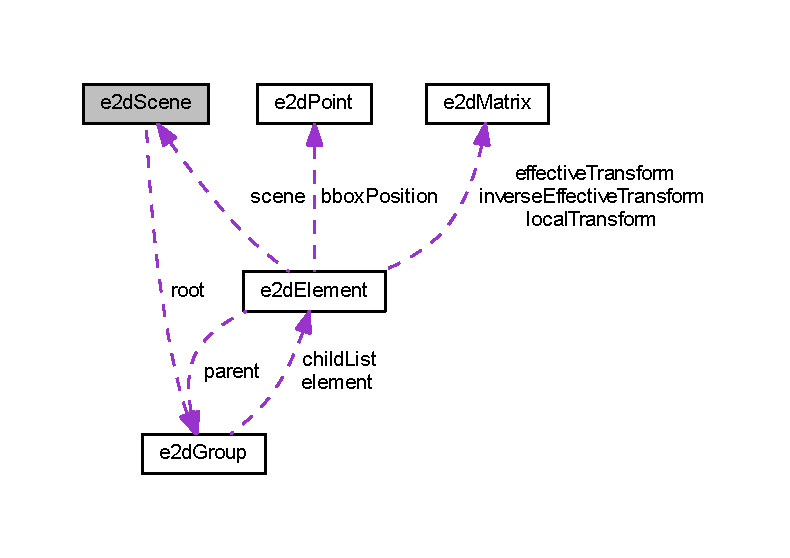
\includegraphics[width=350pt]{structe2dScene__coll__graph}
\end{center}
\end{figure}
\subsection*{Data Fields}
\begin{DoxyCompactItemize}
\item 
\hypertarget{structe2dScene_aa5444ac46bf18449921a4094bcadde1c}{\hyperlink{structe2dGroup}{e2d\-Group} $\ast$ {\bfseries root}}\label{structe2dScene_aa5444ac46bf18449921a4094bcadde1c}

\end{DoxyCompactItemize}


The documentation for this struct was generated from the following file\-:\begin{DoxyCompactItemize}
\item 
e2d\-Scene.\-h\end{DoxyCompactItemize}

\chapter{File Documentation}
\hypertarget{e2dElement_8h}{\section{e2d\-Element.\-h File Reference}
\label{e2dElement_8h}\index{e2d\-Element.\-h@{e2d\-Element.\-h}}
}


File which contains the \hyperlink{structe2dElement}{e2d\-Element} struct and its \char`\"{}methods\char`\"{}.  


{\ttfamily \#include \char`\"{}Ez2\-D\-S.\-h\char`\"{}}\\*
{\ttfamily \#include \char`\"{}e2d\-Matrix.\-h\char`\"{}}\\*
{\ttfamily \#include \char`\"{}e2d\-Point.\-h\char`\"{}}\\*
Include dependency graph for e2d\-Element.\-h\-:\nopagebreak
\begin{figure}[H]
\begin{center}
\leavevmode
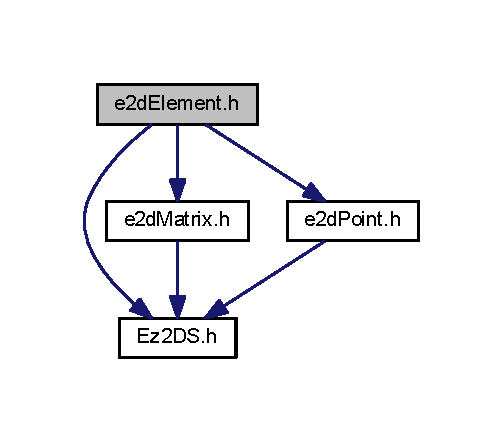
\includegraphics[width=240pt]{e2dElement_8h__incl}
\end{center}
\end{figure}
This graph shows which files directly or indirectly include this file\-:\nopagebreak
\begin{figure}[H]
\begin{center}
\leavevmode
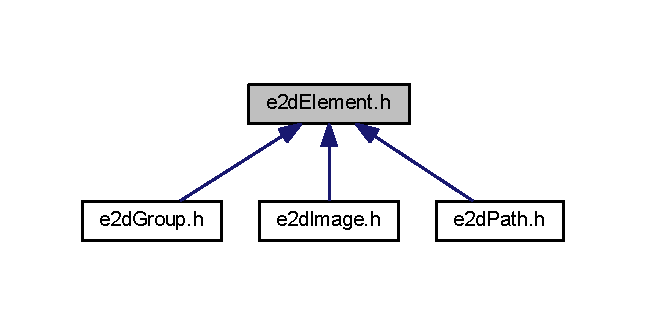
\includegraphics[width=310pt]{e2dElement_8h__dep__incl}
\end{center}
\end{figure}
\subsection*{Data Structures}
\begin{DoxyCompactItemize}
\item 
struct \hyperlink{structe2dElement}{e2d\-Element}
\begin{DoxyCompactList}\small\item\em The \hyperlink{structe2dElement}{e2d\-Element} struct is the base of all elements in the scene. Common scene information such as id, attribute values or transformations are saved in the \hyperlink{structe2dElement}{e2d\-Element} struct. You are not meant to instance this struct by itself. By creating other elements such as \hyperlink{structe2dGroup}{e2d\-Group} or \hyperlink{structe2dImage}{e2d\-Image}, this struct will be automatically allocated in them. This \char`\"{}inheritance\char`\"{} is mimic'd by placing the \hyperlink{structe2dElement}{e2d\-Element} struct as the first element in structs which are meant to be \char`\"{}substructs\char`\"{} of it. \end{DoxyCompactList}\end{DoxyCompactItemize}
\subsection*{Typedefs}
\begin{DoxyCompactItemize}
\item 
\hypertarget{group__e2dElement_ga13e962cd8fa5eaa7d4bec3fc7d774d59}{typedef enum \hyperlink{group__e2dElement_ga9bc8cfdec08c7e9069fc707ee456fd38}{e2d\-Element\-Type} \hyperlink{group__e2dElement_ga13e962cd8fa5eaa7d4bec3fc7d774d59}{e2d\-Element\-Type}}\label{group__e2dElement_ga13e962cd8fa5eaa7d4bec3fc7d774d59}

\begin{DoxyCompactList}\small\item\em The e2d\-Element\-Type enum defines the possible \char`\"{}substructs\char`\"{} of \hyperlink{structe2dElement}{e2d\-Element}. This is used for reflection. \end{DoxyCompactList}\end{DoxyCompactItemize}
\subsection*{Enumerations}
\begin{DoxyCompactItemize}
\item 
enum \hyperlink{group__e2dElement_ga9bc8cfdec08c7e9069fc707ee456fd38}{e2d\-Element\-Type} \{ {\bfseries E2\-D\-\_\-\-G\-R\-O\-U\-P}, 
{\bfseries E2\-D\-\_\-\-P\-A\-T\-H}, 
{\bfseries E2\-D\-\_\-\-I\-M\-A\-G\-E}
 \}
\begin{DoxyCompactList}\small\item\em The e2d\-Element\-Type enum defines the possible \char`\"{}substructs\char`\"{} of \hyperlink{structe2dElement}{e2d\-Element}. This is used for reflection. \end{DoxyCompactList}\end{DoxyCompactItemize}
\subsection*{Functions}
\begin{DoxyCompactItemize}
\item 
void \hyperlink{group__e2dElement_ga8734d10ef40a380dfc51bfe1790a92a7}{e2d\-Element\-Init} (\hyperlink{structe2dElement}{e2d\-Element} $\ast$element, \hyperlink{group__e2dElement_ga9bc8cfdec08c7e9069fc707ee456fd38}{e2d\-Element\-Type} type, const \hyperlink{structe2dScene}{e2d\-Scene} $\ast$scene)
\begin{DoxyCompactList}\small\item\em Called by the create methods of structs which inherit \hyperlink{structe2dElement}{e2d\-Element} (e.\-g. e2d\-Group\-Create). Will initialize all members of the struct with the parameters of this method and with default values on everything else. \end{DoxyCompactList}\item 
void \hyperlink{group__e2dElement_ga214c437a16fe6f3fc795539f851a2019}{e2d\-Element\-Destroy} (\hyperlink{structe2dElement}{e2d\-Element} $\ast$elem)
\begin{DoxyCompactList}\small\item\em Will check the type member of elem and call the appropriate destructor (e.\-g. \hyperlink{group__e2dGroup_ga545626effa0f89b72f244e56aadb05bc}{e2d\-Group\-Destroy()}) \end{DoxyCompactList}\item 
void \hyperlink{group__e2dElement_gae8da5104d70a09549ca74044dda8313c}{e2d\-Element\-Free\-Members} (\hyperlink{structe2dElement}{e2d\-Element} $\ast$elem)
\begin{DoxyCompactList}\small\item\em Will free all the dynamically allocated memory inside the \hyperlink{structe2dElement}{e2d\-Element} struct pointed by elem. \end{DoxyCompactList}\item 
void \hyperlink{group__e2dElement_ga5cfa0a343d3dd1a30b0addc4ec6e7f88}{e2d\-Element\-Add\-Attribute} (\hyperlink{structe2dElement}{e2d\-Element} $\ast$elem, const char $\ast$name, const char $\ast$value)
\begin{DoxyCompactList}\small\item\em Will add an attribute to the element. Increases the size of the array if necessary. \end{DoxyCompactList}\item 
const char $\ast$ \hyperlink{group__e2dElement_gac32ea8a33b317fc014929102d64ac157}{e2d\-Element\-Get\-Attribute} (\hyperlink{structe2dElement}{e2d\-Element} $\ast$elem, const char $\ast$name)
\begin{DoxyCompactList}\small\item\em Returns the value of an attribute with a given name. \end{DoxyCompactList}\item 
\hyperlink{structe2dPoint}{e2d\-Point} \hyperlink{group__e2dElement_ga39dd883e42f609efba3f75300a29ff31}{e2d\-Element\-Get\-Local\-Position} (const \hyperlink{structe2dElement}{e2d\-Element} $\ast$elem)
\begin{DoxyCompactList}\small\item\em Returns the position of the element, taken from the local\-Transform. \end{DoxyCompactList}\item 
\hyperlink{structe2dPoint}{e2d\-Point} \hyperlink{group__e2dElement_ga9b85de42e52c0d89e82f9231ea923c8c}{e2d\-Element\-Get\-World\-Position} (const \hyperlink{structe2dElement}{e2d\-Element} $\ast$elem)
\begin{DoxyCompactList}\small\item\em U\-N\-T\-E\-S\-T\-E\-D Will get the local position (\hyperlink{group__e2dElement_ga39dd883e42f609efba3f75300a29ff31}{e2d\-Element\-Get\-Local\-Position()}) and multiply it by the inverse\-Effective\-Transform and obtain the world position. Needs effective transformations to be calculated ( \hyperlink{group__e2dScene_gac4b32991ff8bab5d5ae429fb97b4e26c}{e2d\-Scene\-Calculate\-Effective\-Transforms()} has been called) \end{DoxyCompactList}\item 
\hyperlink{structe2dPoint}{e2d\-Point} \hyperlink{group__e2dElement_gab4e3f4eeba31c937a946f68617c5cb06}{e2d\-Element\-Get\-Relative\-Position} (const \hyperlink{structe2dElement}{e2d\-Element} $\ast$elem, const \hyperlink{structe2dElement}{e2d\-Element} $\ast$relative\-To)
\begin{DoxyCompactList}\small\item\em U\-N\-T\-E\-S\-T\-E\-D Will get the relative transformation by multiplying the effective transform of elem with the inverse effective transform of relative\-To. The multiply it with the local position of elem (\hyperlink{group__e2dElement_ga39dd883e42f609efba3f75300a29ff31}{e2d\-Element\-Get\-Local\-Position()}). Needs effective transformations to be calculated (\hyperlink{group__e2dScene_gac4b32991ff8bab5d5ae429fb97b4e26c}{e2d\-Scene\-Calculate\-Effective\-Transforms()} has been called) \end{DoxyCompactList}\item 
\hyperlink{structe2dPoint}{e2d\-Point} \hyperlink{group__e2dElement_gac3ad9f8cdc0782378c9f2e93cb7da68f}{e2d\-Element\-Get\-Relative\-Point} (const \hyperlink{structe2dElement}{e2d\-Element} $\ast$elem, const \hyperlink{structe2dElement}{e2d\-Element} $\ast$relative\-To, const \hyperlink{structe2dPoint}{e2d\-Point} $\ast$point)
\begin{DoxyCompactList}\small\item\em U\-N\-T\-E\-S\-T\-E\-D Will get the relative transformation by multiplying the effective transform of elem with the inverse effective transform of relative\-To. The multiply it with point. Needs effective transformations to be calculated (\hyperlink{group__e2dScene_gac4b32991ff8bab5d5ae429fb97b4e26c}{e2d\-Scene\-Calculate\-Effective\-Transforms()} has been called). \end{DoxyCompactList}\item 
void \hyperlink{group__e2dElement_ga94aa710b2da71af2091fe4d5b87ce47e}{e2d\-Element\-Calculate\-Bounding\-Box} (\hyperlink{structe2dElement}{e2d\-Element} $\ast$elem)
\begin{DoxyCompactList}\small\item\em Will check type and calculate the appropriate method (e.\-g. \hyperlink{group__e2dGroup_ga7c5f43489bbd2d36a51414aee07abf5a}{e2d\-Group\-Calculate\-Bounding\-Box()}) \end{DoxyCompactList}\item 
void \hyperlink{group__e2dElement_ga36b01a888c97163c990e16d348aff61c}{e2d\-Element\-Center\-At\-B\-Box} (\hyperlink{structe2dElement}{e2d\-Element} $\ast$elem, float tx, float ty)
\begin{DoxyCompactList}\small\item\em Needs bounding box to have been calculated. Will check type and calculate the appropriate method (e.\-g. \hyperlink{group__e2dGroup_ga04bf94419865ca7f9d6daf30ce3fadf0}{e2d\-Group\-Center\-At\-B\-Box()}). (tx, ty) will define where in the bounding box, the element will be centered, e.\-g. (0,0, will center on the top left corner, (0.\-5, 0.\-5) will center on the center of the bbox. \end{DoxyCompactList}\end{DoxyCompactItemize}


\subsection{Detailed Description}
File which contains the \hyperlink{structe2dElement}{e2d\-Element} struct and its \char`\"{}methods\char`\"{}. \begin{DoxyAuthor}{Author}
Rui (\href{mailto:ruir2c@gmail.com}{\tt ruir2c@gmail.\-com})
\end{DoxyAuthor}
\begin{DoxyDate}{Date}
February, 2012 
\end{DoxyDate}

\hypertarget{e2dGroup_8h}{\section{e2d\-Group.\-h File Reference}
\label{e2dGroup_8h}\index{e2d\-Group.\-h@{e2d\-Group.\-h}}
}


File which contains the \hyperlink{structe2dGroup}{e2d\-Group} struct and its \char`\"{}methods\char`\"{}.  


{\ttfamily \#include \char`\"{}Ez2\-D\-S.\-h\char`\"{}}\\*
{\ttfamily \#include \char`\"{}e2d\-Element.\-h\char`\"{}}\\*
Include dependency graph for e2d\-Group.\-h\-:\nopagebreak
\begin{figure}[H]
\begin{center}
\leavevmode
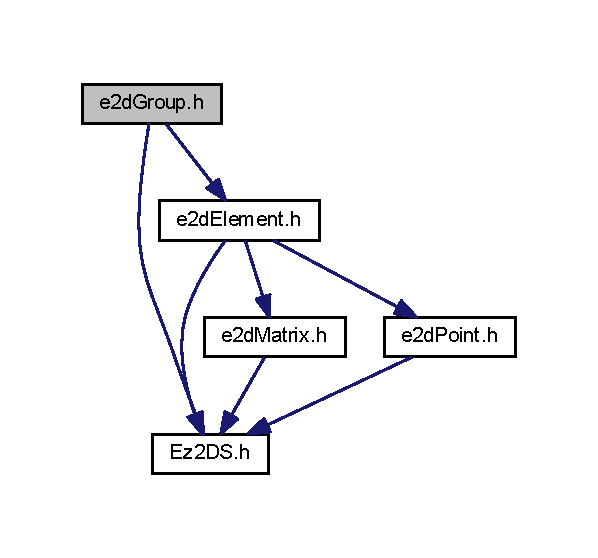
\includegraphics[width=287pt]{e2dGroup_8h__incl}
\end{center}
\end{figure}
\subsection*{Data Structures}
\begin{DoxyCompactItemize}
\item 
struct \hyperlink{structe2dGroup}{e2d\-Group}
\begin{DoxyCompactList}\small\item\em The \hyperlink{structe2dGroup}{e2d\-Group} struct is used to group elements in the scene. This struct is created from the \char`\"{}g\char`\"{} element in S\-V\-G. It \char`\"{}inherits\char`\"{} from \hyperlink{structe2dElement}{e2d\-Element} by placing it as the first element in the struct, if you typecast e2d\-Group$\ast$ into e2d\-Element$\ast$, it will work thus mimicing inheritance in e.\-g. C++. \end{DoxyCompactList}\item 
struct \hyperlink{structe2dGroupIterator}{e2d\-Group\-Iterator}
\begin{DoxyCompactList}\small\item\em An iterator for the children of \hyperlink{structe2dGroup}{e2d\-Group}. \end{DoxyCompactList}\end{DoxyCompactItemize}
\subsection*{Functions}
\begin{DoxyCompactItemize}
\item 
\hyperlink{Ez2DS_8h_a9f14e9cb869e1a85fdaba03afcca0df9}{E2\-D\-\_\-\-E\-X\-P\-O\-R\-T} \hyperlink{structe2dGroup}{e2d\-Group} $\ast$ \hyperlink{group__e2dGroup_ga3c7f6acf28180141c87806a9d260f3f9}{e2d\-Group\-Create} (const \hyperlink{structe2dScene}{e2d\-Scene} $\ast$scene)
\begin{DoxyCompactList}\small\item\em This is the constructor of \hyperlink{structe2dGroup}{e2d\-Group}. It returns a pointer to a new \hyperlink{structe2dGroup}{e2d\-Group}. Inside it calls \hyperlink{group__e2dGroup_gafa3f224a6509fbff5063dc910d4e3f1e}{e2d\-Group\-Init()} to initialize the members of the struct. \end{DoxyCompactList}\item 
\hyperlink{Ez2DS_8h_a9f14e9cb869e1a85fdaba03afcca0df9}{E2\-D\-\_\-\-E\-X\-P\-O\-R\-T} void \hyperlink{group__e2dGroup_gafa3f224a6509fbff5063dc910d4e3f1e}{e2d\-Group\-Init} (\hyperlink{structe2dGroup}{e2d\-Group} $\ast$group, const \hyperlink{structe2dScene}{e2d\-Scene} $\ast$scene)
\begin{DoxyCompactList}\small\item\em This method will initialize the members of the struct, i.\-e. it will allocate the \hyperlink{structe2dGroup_a55f6dde874716dc99dcd270fc0999a01}{e2d\-Group\-::child\-List} array, and call \hyperlink{group__e2dElement_ga8734d10ef40a380dfc51bfe1790a92a7}{e2d\-Element\-Init()}. It is called by \hyperlink{group__e2dGroup_ga3c7f6acf28180141c87806a9d260f3f9}{e2d\-Group\-Create()}. \end{DoxyCompactList}\item 
\hyperlink{Ez2DS_8h_a9f14e9cb869e1a85fdaba03afcca0df9}{E2\-D\-\_\-\-E\-X\-P\-O\-R\-T} void \hyperlink{group__e2dGroup_gae2d96b65c911168dd57442f75c632063}{e2d\-Group\-Destroy} (\hyperlink{structe2dGroup}{e2d\-Group} $\ast$group)
\begin{DoxyCompactList}\small\item\em Calls \hyperlink{group__e2dGroup_gae28cbc879651049422f4045988398b6c}{e2d\-Group\-Free\-Members()}, \hyperlink{group__e2dElement_ga5c3a7d29f41609686a3a455bad6ef7c9}{e2d\-Element\-Free\-Members()}, and then frees the pointer. \hyperlink{group__e2dElement_ga2fdc3435e0e1ac9d1e1f0b330d9539fa}{e2d\-Element\-Destroy()} will call this method. \end{DoxyCompactList}\item 
\hyperlink{Ez2DS_8h_a9f14e9cb869e1a85fdaba03afcca0df9}{E2\-D\-\_\-\-E\-X\-P\-O\-R\-T} void \hyperlink{group__e2dGroup_gae28cbc879651049422f4045988398b6c}{e2d\-Group\-Free\-Members} (\hyperlink{structe2dGroup}{e2d\-Group} $\ast$group)
\begin{DoxyCompactList}\small\item\em Will free all the dynamically allocated memory inside the \hyperlink{structe2dGroup}{e2d\-Group} struct pointed by elem, i.\-e. it calls \hyperlink{group__e2dElement_ga2fdc3435e0e1ac9d1e1f0b330d9539fa}{e2d\-Element\-Destroy()} on all the children, and frees the \hyperlink{structe2dGroup_a55f6dde874716dc99dcd270fc0999a01}{e2d\-Group\-::child\-List} array (Warning, this might change in future versions). It is called by \hyperlink{group__e2dGroup_gae2d96b65c911168dd57442f75c632063}{e2d\-Group\-Destroy()}. \end{DoxyCompactList}\item 
\hyperlink{Ez2DS_8h_a9f14e9cb869e1a85fdaba03afcca0df9}{E2\-D\-\_\-\-E\-X\-P\-O\-R\-T} void \hyperlink{group__e2dGroup_ga364ad3636ddb85fafbd8817b4d6e2c1d}{e2d\-Group\-Add\-Child} (\hyperlink{structe2dGroup}{e2d\-Group} $\ast$group, \hyperlink{structe2dElement}{e2d\-Element} $\ast$element)
\begin{DoxyCompactList}\small\item\em Will add an element to the \hyperlink{structe2dGroup_a55f6dde874716dc99dcd270fc0999a01}{e2d\-Group\-::child\-List} array, increasing allocated space if necessary. Also sets \hyperlink{structe2dElement_a3e62eb2fbf1d6bc6d6fe549096a6cee9}{e2d\-Element\-::parent} in \char`\"{}element\char`\"{} to be \char`\"{}group\char`\"{}. \end{DoxyCompactList}\item 
\hyperlink{Ez2DS_8h_a9f14e9cb869e1a85fdaba03afcca0df9}{E2\-D\-\_\-\-E\-X\-P\-O\-R\-T} void \hyperlink{group__e2dGroup_gacf5659083b312e030456721b2560d4f4}{e2d\-Group\-Calculate\-Bounding\-Box} (\hyperlink{structe2dGroup}{e2d\-Group} $\ast$group)
\begin{DoxyCompactList}\small\item\em Calculates the bounding box of the group using the bounding boxes of the children. If a child doesn't have the bounding box calculated, then \hyperlink{group__e2dElement_ga575c7363927670f1ea8c52b7ea23fcd5}{e2d\-Element\-Calculate\-Bounding\-Box()} is called in the child. \end{DoxyCompactList}\item 
\hyperlink{Ez2DS_8h_a9f14e9cb869e1a85fdaba03afcca0df9}{E2\-D\-\_\-\-E\-X\-P\-O\-R\-T} void \hyperlink{group__e2dGroup_ga2800a7dc3827e8753e2f2c6ef2e05eb9}{e2d\-Group\-Center\-At\-B\-Box} (\hyperlink{structe2dGroup}{e2d\-Group} $\ast$group, float tx, float ty)
\begin{DoxyCompactList}\small\item\em Adds a transformation to the group which subtracts the position of the Bounding Box (offset by (tx, ty)), and adds the position of the bounding box to all the children, effectively bringing the origin of the local coordinate system to the bounding box. See \hyperlink{group__e2dElement_gab829b280fa22a3509c40425fc84b5061}{e2d\-Element\-Center\-At\-B\-Box()} for an explanation on \char`\"{}tx\char`\"{} and \char`\"{}ty\char`\"{}. \end{DoxyCompactList}\item 
\hyperlink{Ez2DS_8h_a9f14e9cb869e1a85fdaba03afcca0df9}{E2\-D\-\_\-\-E\-X\-P\-O\-R\-T} void \hyperlink{group__e2dGroup_ga406ebab73c321b771a9a58e26c3a5d79}{e2d\-Group\-Flatten} (\hyperlink{structe2dGroup}{e2d\-Group} $\ast$group)
\begin{DoxyCompactList}\small\item\em Recursively removes all the groups which are children (directly or indirectly) and makes all the remaining elements have a \hyperlink{structe2dElement_a52bda732df714953f93c1e6f5f7c7c93}{e2d\-Element\-::local\-Transform} which yields a transformation equal to if there were groups. I.\-e., it flattens the group, making it have only one level. Calling this on the \hyperlink{structe2dScene_aa5444ac46bf18449921a4094bcadde1c}{e2d\-Scene\-::root} will make \char`\"{}group\char`\"{} be the only in the tree. !!\-Warning!! custom (and non custom) tags written in groups are lost! \end{DoxyCompactList}\item 
\hyperlink{Ez2DS_8h_a9f14e9cb869e1a85fdaba03afcca0df9}{E2\-D\-\_\-\-E\-X\-P\-O\-R\-T} \hyperlink{structe2dGroupIterator}{e2d\-Group\-Iterator} \hyperlink{group__e2dGroup_ga35b130caa1b107616881615e9c8fb9ad}{e2d\-Group\-Get\-Child\-Iterator} (\hyperlink{structe2dGroup}{e2d\-Group} $\ast$group)
\begin{DoxyCompactList}\small\item\em Makes an iterator to the children of the group. \end{DoxyCompactList}\item 
\hyperlink{Ez2DS_8h_a9f14e9cb869e1a85fdaba03afcca0df9}{E2\-D\-\_\-\-E\-X\-P\-O\-R\-T} \hyperlink{structe2dElement}{e2d\-Element} $\ast$ \hyperlink{group__e2dGroup_ga5a20617c4666d240ab6c0efdde72d23f}{e2d\-Group\-Iterator\-Next} (\hyperlink{structe2dGroupIterator}{e2d\-Group\-Iterator} $\ast$iter)
\begin{DoxyCompactList}\small\item\em Returns the current child and advances. \end{DoxyCompactList}\item 
\hyperlink{Ez2DS_8h_a9f14e9cb869e1a85fdaba03afcca0df9}{E2\-D\-\_\-\-E\-X\-P\-O\-R\-T} \hyperlink{Ez2DS_8h_aac8cdc3a3bcd6b56a8c3e0bb6979cbf8}{E2\-D\-\_\-\-B\-O\-O\-L} \hyperlink{group__e2dGroup_ga2e74310ea432fa45cea8b03da8fc29ef}{e2d\-Group\-Iterator\-Has\-Next} (\hyperlink{structe2dGroupIterator}{e2d\-Group\-Iterator} $\ast$iter)
\begin{DoxyCompactList}\small\item\em Checks if we have a child at current element pointed by iter, if not, we have reached the end of the child list. \end{DoxyCompactList}\end{DoxyCompactItemize}


\subsection{Detailed Description}
File which contains the \hyperlink{structe2dGroup}{e2d\-Group} struct and its \char`\"{}methods\char`\"{}. \begin{DoxyAuthor}{Author}
Rui (\href{mailto:ruir2c@gmail.com}{\tt ruir2c@gmail.\-com})
\end{DoxyAuthor}
\begin{DoxyDate}{Date}
February, 2012 
\end{DoxyDate}

\hypertarget{e2dImage_8h}{\section{e2d\-Image.\-h File Reference}
\label{e2dImage_8h}\index{e2d\-Image.\-h@{e2d\-Image.\-h}}
}


File which contains the \hyperlink{structe2dImage}{e2d\-Image} struct and its \char`\"{}methods\char`\"{}.  


{\ttfamily \#include \char`\"{}Ez2\-D\-S.\-h\char`\"{}}\\*
{\ttfamily \#include \char`\"{}e2d\-Element.\-h\char`\"{}}\\*
Include dependency graph for e2d\-Image.\-h\-:
\nopagebreak
\begin{figure}[H]
\begin{center}
\leavevmode
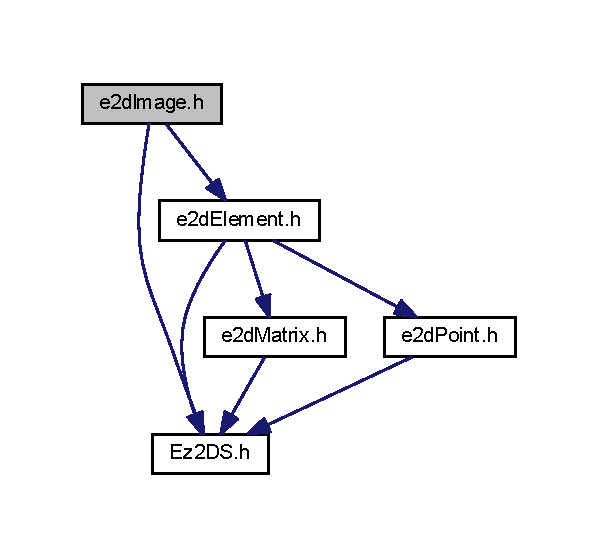
\includegraphics[width=287pt]{e2dImage_8h__incl}
\end{center}
\end{figure}
\subsection*{Data Structures}
\begin{DoxyCompactItemize}
\item 
struct \hyperlink{structe2dImage}{e2d\-Image}
\begin{DoxyCompactList}\small\item\em The \hyperlink{structe2dImage}{e2d\-Image} struct is used for holding the paths to images and their size and position. The struct is composed directly from the contents of the S\-V\-G image element. It \char`\"{}inherits\char`\"{} from \hyperlink{structe2dElement}{e2d\-Element} by placing it as the first element in the struct, if you typecast e2d\-Struct$\ast$ into e2d\-Element$\ast$, it will work thus mimicing inheritance in e.\-g. C++. \end{DoxyCompactList}\end{DoxyCompactItemize}
\subsection*{Functions}
\begin{DoxyCompactItemize}
\item 
\hyperlink{structe2dImage}{e2d\-Image} $\ast$ \hyperlink{group__e2dImage_gafc7e085a237f8d2f1b147b3cca8259d6}{e2d\-Image\-Create} (const \hyperlink{structe2dScene}{e2d\-Scene} $\ast$scene)
\begin{DoxyCompactList}\small\item\em This is the constructor of \hyperlink{structe2dImage}{e2d\-Image}. It returns a pointer to a new \hyperlink{structe2dImage}{e2d\-Image}. Inside it calls \hyperlink{group__e2dImage_ga11703b45867fb00d56489a3a6bc6bb9c}{e2d\-Image\-Init()} to initialize the members of the struct. \end{DoxyCompactList}\item 
void \hyperlink{group__e2dImage_ga11703b45867fb00d56489a3a6bc6bb9c}{e2d\-Image\-Init} (\hyperlink{structe2dImage}{e2d\-Image} $\ast$image, const \hyperlink{structe2dScene}{e2d\-Scene} $\ast$scene)
\begin{DoxyCompactList}\small\item\em This method will initialize the members of the struct, i.\-e. it will zero the members, and call \hyperlink{group__e2dElement_ga8734d10ef40a380dfc51bfe1790a92a7}{e2d\-Element\-Init()}. It is called by \hyperlink{group__e2dImage_gafc7e085a237f8d2f1b147b3cca8259d6}{e2d\-Image\-Create()}. \end{DoxyCompactList}\item 
void \hyperlink{group__e2dImage_gacf174e48578f0e23888e37f47a3ef10b}{e2d\-Image\-Destroy} (\hyperlink{structe2dImage}{e2d\-Image} $\ast$image)
\begin{DoxyCompactList}\small\item\em Calls \hyperlink{group__e2dImage_gaf5409c0b10e8a8d8b9bd3f08e1d5da1f}{e2d\-Image\-Free\-Members()}, \hyperlink{group__e2dElement_gae8da5104d70a09549ca74044dda8313c}{e2d\-Element\-Free\-Members()}, and then frees the pointer. \hyperlink{group__e2dElement_ga214c437a16fe6f3fc795539f851a2019}{e2d\-Element\-Destroy()} will call this method. \end{DoxyCompactList}\item 
void \hyperlink{group__e2dImage_gaf5409c0b10e8a8d8b9bd3f08e1d5da1f}{e2d\-Image\-Free\-Members} (\hyperlink{structe2dImage}{e2d\-Image} $\ast$image)
\begin{DoxyCompactList}\small\item\em Will free all the allocated memory inside the \hyperlink{structe2dImage}{e2d\-Image} struct pointed by elem, i.\-e. it checks if \hyperlink{structe2dImage_afb14ab23ba86115c3b01ad4122943f89}{e2d\-Image\-::image\-Path} has been defined and frees the pointer. It is called by \hyperlink{group__e2dImage_gacf174e48578f0e23888e37f47a3ef10b}{e2d\-Image\-Destroy()}. \end{DoxyCompactList}\item 
void \hyperlink{group__e2dImage_ga6df4ef2b71e130f5817b079b6b32d249}{e2d\-Image\-Calculate\-Bounding\-Box} (\hyperlink{structe2dImage}{e2d\-Image} $\ast$image)
\begin{DoxyCompactList}\small\item\em A quite straight forward function which simply makes the \hyperlink{structe2dImage_ae426f00e82704fa09578f5446e22d915}{e2d\-Image\-::width}, \hyperlink{structe2dImage_a48083b65ac9a863566dc3e3fff09a5b4}{e2d\-Image\-::height} and \hyperlink{structe2dImage_afa8983f25fd6aa6aca18feb07d8d2249}{e2d\-Image\-::position} of the image also be the bounding box. If a \hyperlink{structe2dImage_ae426f00e82704fa09578f5446e22d915}{e2d\-Image\-::width} and \hyperlink{structe2dImage_a48083b65ac9a863566dc3e3fff09a5b4}{e2d\-Image\-::height} is not supplied, the bounding box won't be calculated. We can't check the actual image size as that would bring additional dependencies to the library, so be careful with it. \end{DoxyCompactList}\item 
void \hyperlink{group__e2dImage_ga08652fd1ad70d4935d98bcc02a38fb69}{e2d\-Image\-Center\-At\-B\-Box} (\hyperlink{structe2dImage}{e2d\-Image} $\ast$image, float tx, float ty)
\begin{DoxyCompactList}\small\item\em Adds a transformation to the image which subtracts the position (offset by (tx,ty)) of the Bounding Box, and adds the position of the bounding box to the image position, effectively bringing the origin of the local coordinate system to the bounding box. See \hyperlink{group__e2dElement_ga36b01a888c97163c990e16d348aff61c}{e2d\-Element\-Center\-At\-B\-Box()} for an explanation on \char`\"{}tx\char`\"{} and \char`\"{}ty\char`\"{}. \end{DoxyCompactList}\end{DoxyCompactItemize}


\subsection{Detailed Description}
File which contains the \hyperlink{structe2dImage}{e2d\-Image} struct and its \char`\"{}methods\char`\"{}. \begin{DoxyAuthor}{Author}
Rui (\href{mailto:ruir2c@gmail.com}{\tt ruir2c@gmail.\-com})
\end{DoxyAuthor}
\begin{DoxyDate}{Date}
February, 2012 
\end{DoxyDate}

\hypertarget{e2dMatrix_8h}{\section{e2d\-Matrix.\-h File Reference}
\label{e2dMatrix_8h}\index{e2d\-Matrix.\-h@{e2d\-Matrix.\-h}}
}


File which contains a 3x3 matrix implementation and utility methods.  


{\ttfamily \#include \char`\"{}Ez2\-D\-S.\-h\char`\"{}}\\*
Include dependency graph for e2d\-Matrix.\-h\-:
\nopagebreak
\begin{figure}[H]
\begin{center}
\leavevmode
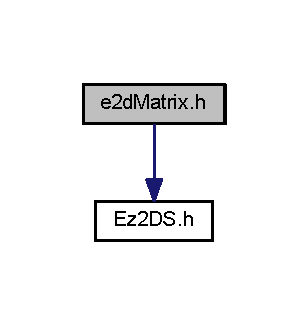
\includegraphics[width=148pt]{e2dMatrix_8h__incl}
\end{center}
\end{figure}
This graph shows which files directly or indirectly include this file\-:
\nopagebreak
\begin{figure}[H]
\begin{center}
\leavevmode
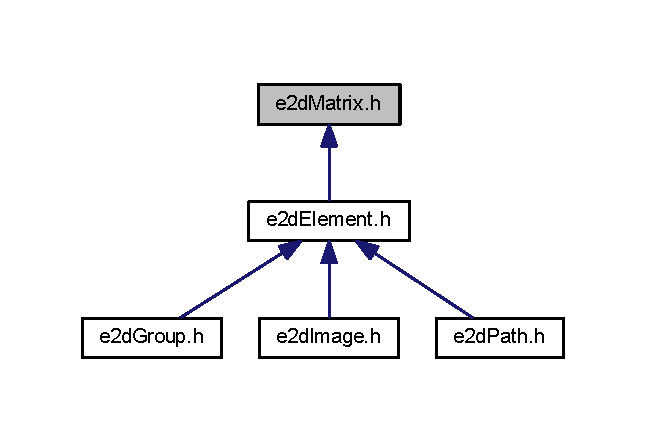
\includegraphics[width=310pt]{e2dMatrix_8h__dep__incl}
\end{center}
\end{figure}
\subsection*{Data Structures}
\begin{DoxyCompactItemize}
\item 
struct \hyperlink{structe2dMatrix}{e2d\-Matrix}
\begin{DoxyCompactList}\small\item\em The \hyperlink{structe2dMatrix}{e2d\-Matrix} struct contains the implementation of a 3x3 matrix which is row major. See \href{http://en.wikipedia.org/wiki/Row-major_order}{\tt http\-://en.\-wikipedia.\-org/wiki/\-Row-\/major\-\_\-order} if you have doubts. \end{DoxyCompactList}\end{DoxyCompactItemize}
\subsection*{Functions}
\begin{DoxyCompactItemize}
\item 
\hypertarget{group__e2dMatrix_gae071d0d13c408d0faa8ea81731a47746}{void \hyperlink{group__e2dMatrix_gae071d0d13c408d0faa8ea81731a47746}{e2d\-Matrix\-To\-Ident} (\hyperlink{structe2dMatrix}{e2d\-Matrix} $\ast$mat)}\label{group__e2dMatrix_gae071d0d13c408d0faa8ea81731a47746}

\begin{DoxyCompactList}\small\item\em Sets mat to be identity, basically assigns E2\-D\-\_\-\-I\-D\-E\-N\-T\-\_\-\-M\-A\-T\-R\-I\-X. \end{DoxyCompactList}\item 
\hypertarget{group__e2dMatrix_gab5e5b40fd56f6fde5ec19e09733ddb35}{void \hyperlink{group__e2dMatrix_gab5e5b40fd56f6fde5ec19e09733ddb35}{e2d\-Matrix\-Set\-Col} (\hyperlink{structe2dMatrix}{e2d\-Matrix} $\ast$mat, unsigned int col, float val1, float val2, float val3)}\label{group__e2dMatrix_gab5e5b40fd56f6fde5ec19e09733ddb35}

\begin{DoxyCompactList}\small\item\em Changes the column defined by col (0 to 2) to be val1, val2 and val3. \end{DoxyCompactList}\item 
\hypertarget{group__e2dMatrix_gaca877ffd79967e78914eb5fea731300b}{void \hyperlink{group__e2dMatrix_gaca877ffd79967e78914eb5fea731300b}{e2d\-Matrix\-Set\-Row} (\hyperlink{structe2dMatrix}{e2d\-Matrix} $\ast$mat, unsigned int row, float val1, float val2, float val3)}\label{group__e2dMatrix_gaca877ffd79967e78914eb5fea731300b}

\begin{DoxyCompactList}\small\item\em Changes the row defined by row (0 to 2) to be val1, val2 and val3. \end{DoxyCompactList}\item 
\hypertarget{group__e2dMatrix_ga5719742adf7b07c791323de17be257a9}{void \hyperlink{group__e2dMatrix_ga5719742adf7b07c791323de17be257a9}{e2d\-Matrix\-Set\-Row\-Col} (\hyperlink{structe2dMatrix}{e2d\-Matrix} $\ast$mat, unsigned int row, unsigned int col, float val1)}\label{group__e2dMatrix_ga5719742adf7b07c791323de17be257a9}

\begin{DoxyCompactList}\small\item\em Changes the position in row \char`\"{}row\char`\"{}, column \char`\"{}col\char`\"{} to be val1. \end{DoxyCompactList}\item 
float \hyperlink{group__e2dMatrix_ga83e3deb8c27d5e63cd03a21930df0c94}{e2d\-Matrix\-Get\-Cell} (const \hyperlink{structe2dMatrix}{e2d\-Matrix} $\ast$mat, unsigned int row, unsigned int col)
\begin{DoxyCompactList}\small\item\em Returns the cell in row \char`\"{}row\char`\"{}, column \char`\"{}column\char`\"{}. \end{DoxyCompactList}\item 
\hyperlink{structe2dMatrix}{e2d\-Matrix} \hyperlink{group__e2dMatrix_gabb941a9a10fba12867cf6e4047bcefcc}{e2d\-Matrix\-Multiply} (const \hyperlink{structe2dMatrix}{e2d\-Matrix} $\ast$mat, const \hyperlink{structe2dMatrix}{e2d\-Matrix} $\ast$multiplicator)
\begin{DoxyCompactList}\small\item\em Multiplies the mat by multiplicator and returns the result in another matrix. \end{DoxyCompactList}\item 
\hypertarget{group__e2dMatrix_ga9c4bc2c260d552037b8d183ecb5dd698}{void \hyperlink{group__e2dMatrix_ga9c4bc2c260d552037b8d183ecb5dd698}{e2d\-Matrix\-Set\-As\-Translation} (\hyperlink{structe2dMatrix}{e2d\-Matrix} $\ast$mat, float x, float y)}\label{group__e2dMatrix_ga9c4bc2c260d552037b8d183ecb5dd698}

\begin{DoxyCompactList}\small\item\em Places an identity matrix and sets first and second row's last cell to be x and y respectively. \end{DoxyCompactList}\item 
\hypertarget{group__e2dMatrix_ga9812a9edb91395ad042ce4475c55060f}{void \hyperlink{group__e2dMatrix_ga9812a9edb91395ad042ce4475c55060f}{e2d\-Matrix\-Set\-As\-Scale} (\hyperlink{structe2dMatrix}{e2d\-Matrix} $\ast$mat, float x, float y)}\label{group__e2dMatrix_ga9812a9edb91395ad042ce4475c55060f}

\begin{DoxyCompactList}\small\item\em Places an identity matrix and sets cell (0,0) and (1,1) to be x and y respectively. \end{DoxyCompactList}\item 
\hypertarget{group__e2dMatrix_ga671b90f626035724fcf0f43d352ec3ad}{void \hyperlink{group__e2dMatrix_ga671b90f626035724fcf0f43d352ec3ad}{e2d\-Matrix\-Set\-As\-Rotation} (\hyperlink{structe2dMatrix}{e2d\-Matrix} $\ast$mat, float radians)}\label{group__e2dMatrix_ga671b90f626035724fcf0f43d352ec3ad}

\begin{DoxyCompactList}\small\item\em Places an identity matrix and sets a rotation according to \href{http://en.wikipedia.org/wiki/Rotation_matrix}{\tt http\-://en.\-wikipedia.\-org/wiki/\-Rotation\-\_\-matrix}. \end{DoxyCompactList}\item 
\hyperlink{structe2dMatrix}{e2d\-Matrix} \hyperlink{group__e2dMatrix_ga86a7cb5c0d6fce078ed754195e8fe1e4}{e2d\-Matrix\-Get\-Inverse} (const \hyperlink{structe2dMatrix}{e2d\-Matrix} $\ast$mat)
\begin{DoxyCompactList}\small\item\em Inverts the matrix using Cramer's rule (see \href{http://en.wikipedia.org/wiki/Cramer%27s_rule}{\tt http\-://en.\-wikipedia.\-org/wiki/\-Cramer\%27s\-\_\-rule}) and returns the result. \end{DoxyCompactList}\item 
\hyperlink{structe2dPoint}{e2d\-Point} \hyperlink{group__e2dMatrix_ga377eea18be8a4e88dcba9c62bffea97e}{e2d\-Matrix\-Apply\-To\-Point} (const \hyperlink{structe2dMatrix}{e2d\-Matrix} $\ast$mat, const \hyperlink{structe2dPoint}{e2d\-Point} $\ast$point)
\begin{DoxyCompactList}\small\item\em Applies the matrix to the point transforming it. \end{DoxyCompactList}\end{DoxyCompactItemize}


\subsection{Detailed Description}
File which contains a 3x3 matrix implementation and utility methods. \begin{DoxyAuthor}{Author}
Rui (\href{mailto:ruir2c@gmail.com}{\tt ruir2c@gmail.\-com})
\end{DoxyAuthor}
\begin{DoxyDate}{Date}
February, 2012 
\end{DoxyDate}

\hypertarget{e2dPoint_8h}{\section{e2d\-Point.\-h File Reference}
\label{e2dPoint_8h}\index{e2d\-Point.\-h@{e2d\-Point.\-h}}
}


File which contains a struct definition of a point (two floats).  


{\ttfamily \#include \char`\"{}Ez2\-D\-S.\-h\char`\"{}}\\*
Include dependency graph for e2d\-Point.\-h\-:
\nopagebreak
\begin{figure}[H]
\begin{center}
\leavevmode
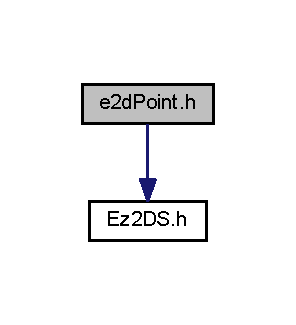
\includegraphics[width=142pt]{e2dPoint_8h__incl}
\end{center}
\end{figure}
This graph shows which files directly or indirectly include this file\-:
\nopagebreak
\begin{figure}[H]
\begin{center}
\leavevmode
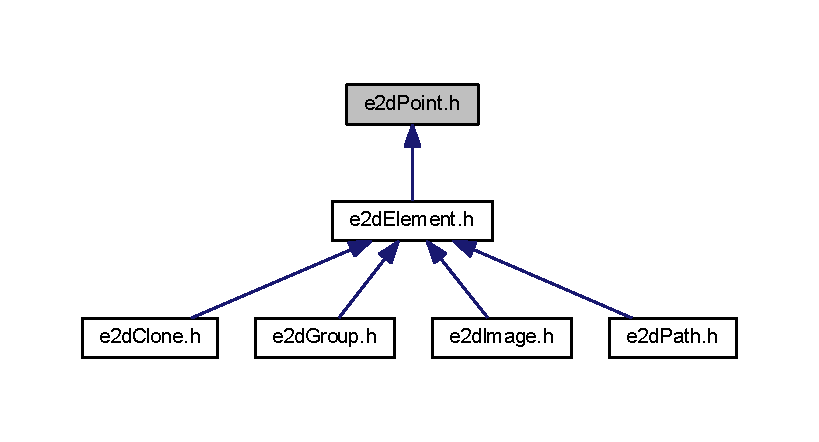
\includegraphics[width=310pt]{e2dPoint_8h__dep__incl}
\end{center}
\end{figure}
\subsection*{Data Structures}
\begin{DoxyCompactItemize}
\item 
struct \hyperlink{structe2dPoint}{e2d\-Point}
\begin{DoxyCompactList}\small\item\em The \hyperlink{structe2dPoint}{e2d\-Point} struct which contains two floats. \end{DoxyCompactList}\end{DoxyCompactItemize}


\subsection{Detailed Description}
File which contains a struct definition of a point (two floats). \begin{DoxyAuthor}{Author}
Rui (\href{mailto:ruir2c@gmail.com}{\tt ruir2c@gmail.\-com})
\end{DoxyAuthor}
\begin{DoxyDate}{Date}
February, 2012 
\end{DoxyDate}

\hypertarget{e2dScene_8h}{\section{e2d\-Scene.\-h File Reference}
\label{e2dScene_8h}\index{e2d\-Scene.\-h@{e2d\-Scene.\-h}}
}


File which contains the \hyperlink{structe2dScene}{e2d\-Scene} struct and its \char`\"{}methods\char`\"{}.  


{\ttfamily \#include \char`\"{}Ez2\-D\-S.\-h\char`\"{}}\\*
Include dependency graph for e2d\-Scene.\-h\-:\nopagebreak
\begin{figure}[H]
\begin{center}
\leavevmode
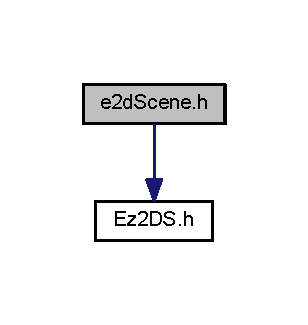
\includegraphics[width=148pt]{e2dScene_8h__incl}
\end{center}
\end{figure}
\subsection*{Data Structures}
\begin{DoxyCompactItemize}
\item 
struct \hyperlink{structe2dScene}{e2d\-Scene}
\begin{DoxyCompactList}\small\item\em The \hyperlink{structe2dScene}{e2d\-Scene} struct defines a scene obtained from an S\-V\-G file. The struct contains the root under which all the objects in the scene can be accessed. \end{DoxyCompactList}\end{DoxyCompactItemize}
\subsection*{Functions}
\begin{DoxyCompactItemize}
\item 
\hyperlink{Ez2DS_8h_a9f14e9cb869e1a85fdaba03afcca0df9}{E2\-D\-\_\-\-E\-X\-P\-O\-R\-T} void \hyperlink{group__e2dScene_ga6981f2448904c96723449cb84ffb4d8a}{e2d\-Scene\-Calculate\-Effective\-Transforms} (\hyperlink{structe2dScene}{e2d\-Scene} $\ast$scene)
\begin{DoxyCompactList}\small\item\em Assigns the effective transform (calculated by multiplying the local transform with the effective transform of the parent element) to every element in the scene. It is useful to have this information for calculating relative positions(for example, knowing world positions, or positions of elements relative to other elements. \end{DoxyCompactList}\item 
\hyperlink{Ez2DS_8h_a9f14e9cb869e1a85fdaba03afcca0df9}{E2\-D\-\_\-\-E\-X\-P\-O\-R\-T} void \hyperlink{group__e2dScene_ga1d33ba7ce041a68b061cfa6b0291b886}{e2d\-Scene\-Center\-All\-At\-B\-Box} (\hyperlink{structe2dScene}{e2d\-Scene} $\ast$scene, float tx, float ty)
\begin{DoxyCompactList}\small\item\em Calls e2d\-Element\-Center\-At\-B\-Box on all the elements in the scene. Needs Bounding Boxes to have been calculated. See \hyperlink{group__e2dGroup_ga2800a7dc3827e8753e2f2c6ef2e05eb9}{e2d\-Group\-Center\-At\-B\-Box()} for an explanation on the tx and ty parameters. \end{DoxyCompactList}\item 
\hyperlink{Ez2DS_8h_a9f14e9cb869e1a85fdaba03afcca0df9}{E2\-D\-\_\-\-E\-X\-P\-O\-R\-T} void \hyperlink{group__e2dScene_gaa202610ee0b2e5c47bded576b365c195}{e2d\-Scene\-Calculate\-All\-B\-Box} (\hyperlink{structe2dScene}{e2d\-Scene} $\ast$scene)
\begin{DoxyCompactList}\small\item\em Calls e2d\-Group\-Calculate\-B\-Box() on the root of the scene. \end{DoxyCompactList}\item 
\hyperlink{Ez2DS_8h_a9f14e9cb869e1a85fdaba03afcca0df9}{E2\-D\-\_\-\-E\-X\-P\-O\-R\-T} \hyperlink{structe2dScene}{e2d\-Scene} $\ast$ \hyperlink{group__e2dScene_ga9994e9f2692c5007b91d02c19350cd1b}{create\-Scene\-From\-File} (char $\ast$file)
\begin{DoxyCompactList}\small\item\em Reads the S\-V\-G in the path \char`\"{}file\char`\"{} using Mini\-X\-M\-L (\href{http://minixml.org/}{\tt http\-://minixml.\-org/}) and creates a \hyperlink{structe2dScene}{e2d\-Scene} struct which is returned. \end{DoxyCompactList}\end{DoxyCompactItemize}


\subsection{Detailed Description}
File which contains the \hyperlink{structe2dScene}{e2d\-Scene} struct and its \char`\"{}methods\char`\"{}. \begin{DoxyAuthor}{Author}
Rui (\href{mailto:ruir2c@gmail.com}{\tt ruir2c@gmail.\-com})
\end{DoxyAuthor}
\begin{DoxyDate}{Date}
February, 2012 
\end{DoxyDate}

\hypertarget{Ez2DS_8h}{\section{Ez2\-D\-S.\-h File Reference}
\label{Ez2DS_8h}\index{Ez2\-D\-S.\-h@{Ez2\-D\-S.\-h}}
}


File which contains global definitions useful to be included on every other file of the library. These definitions include forward declaration of all the structs, and some utility functions.  


This graph shows which files directly or indirectly include this file\-:
\nopagebreak
\begin{figure}[H]
\begin{center}
\leavevmode
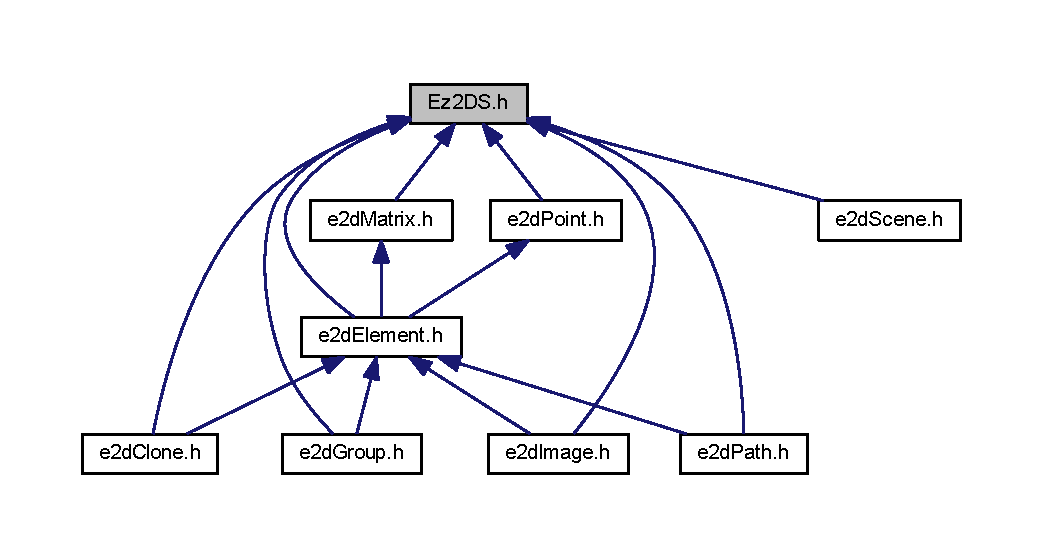
\includegraphics[width=350pt]{Ez2DS_8h__dep__incl}
\end{center}
\end{figure}
\subsection*{Defines}
\begin{DoxyCompactItemize}
\item 
\#define \hyperlink{Ez2DS_8h_a48ffc9ed217e38fc9cd7cf8f9894d63c}{E2\-D\-\_\-\-A\-L\-M\-O\-S\-T\-\_\-\-Z\-E\-R\-O}~1.\-0e-\/6f
\begin{DoxyCompactList}\small\item\em Defines a value which is almost zero. \end{DoxyCompactList}\item 
\#define \hyperlink{Ez2DS_8h_a5f5051e054baa41a7a7048bd205bc1e3}{E2\-D\-\_\-\-I\-S\-\_\-\-A\-L\-M\-O\-S\-T\-\_\-\-Z\-E\-R\-O}(val)~((val) $<$ (\hyperlink{Ez2DS_8h_a48ffc9ed217e38fc9cd7cf8f9894d63c}{E2\-D\-\_\-\-A\-L\-M\-O\-S\-T\-\_\-\-Z\-E\-R\-O}) \&\& (val) $>$ -\/(\hyperlink{Ez2DS_8h_a48ffc9ed217e38fc9cd7cf8f9894d63c}{E2\-D\-\_\-\-A\-L\-M\-O\-S\-T\-\_\-\-Z\-E\-R\-O}))
\begin{DoxyCompactList}\small\item\em Checks if val is within the threshold defined by E2\-D\-\_\-\-A\-L\-M\-O\-S\-T\-\_\-\-Z\-E\-R\-O, i.\-e. it checks if val is below E2\-D\-\_\-\-A\-L\-M\-O\-S\-T\-\_\-\-Z\-E\-R\-O and above -\/ E2\-D\-\_\-\-A\-L\-M\-O\-S\-T\-\_\-\-Z\-E\-R\-O. \end{DoxyCompactList}\item 
\hypertarget{Ez2DS_8h_ae6c89cca978cb0aa64dc7034b016f5cd}{\#define \hyperlink{Ez2DS_8h_ae6c89cca978cb0aa64dc7034b016f5cd}{E2\-D\-\_\-\-N\-U\-L\-L}~0}\label{Ez2DS_8h_ae6c89cca978cb0aa64dc7034b016f5cd}

\begin{DoxyCompactList}\small\item\em N\-U\-L\-L definition. \end{DoxyCompactList}\item 
\#define \hyperlink{Ez2DS_8h_a1cd9ecc64e25100eeb04dc1b08c28fc1}{E2\-D\-\_\-\-M\-A\-X}(a, b)
\begin{DoxyCompactList}\small\item\em Returns the biggest number between a and b. \end{DoxyCompactList}\item 
\#define \hyperlink{Ez2DS_8h_af5964c56c46211897a998a087d4c3a66}{E2\-D\-\_\-\-M\-I\-N}(a, b)
\begin{DoxyCompactList}\small\item\em Returns the smallest number between a and b. \end{DoxyCompactList}\end{DoxyCompactItemize}
\subsection*{Typedefs}
{\bf }\par
\begin{DoxyCompactItemize}
\item 
\hypertarget{Ez2DS_8h_a4663bede7d265bce67f2176cbe6d1f97}{typedef struct \hyperlink{structe2dScene}{e2d\-Scene} \hyperlink{Ez2DS_8h_a4663bede7d265bce67f2176cbe6d1f97}{e2d\-Scene}}\label{Ez2DS_8h_a4663bede7d265bce67f2176cbe6d1f97}

\begin{DoxyCompactList}\small\item\em Forward declarations \begin{DoxyVerb}  \end{DoxyVerb}
. \end{DoxyCompactList}\item 
\hypertarget{Ez2DS_8h_a7d730be997ced9a362d3fbde0c925029}{typedef struct \hyperlink{structe2dElement}{e2d\-Element} {\bfseries e2d\-Element}}\label{Ez2DS_8h_a7d730be997ced9a362d3fbde0c925029}

\item 
\hypertarget{Ez2DS_8h_af3a345c79086b4c4a3bef68d54ec75bb}{typedef struct \hyperlink{structe2dGroup}{e2d\-Group} {\bfseries e2d\-Group}}\label{Ez2DS_8h_af3a345c79086b4c4a3bef68d54ec75bb}

\item 
\hypertarget{Ez2DS_8h_ae4c99476350936b6317aad7ddad92e87}{typedef struct \hyperlink{structe2dPath}{e2d\-Path} {\bfseries e2d\-Path}}\label{Ez2DS_8h_ae4c99476350936b6317aad7ddad92e87}

\item 
\hypertarget{Ez2DS_8h_ac6e31ed0b788ebe46ab4fe4e3f94f0e8}{typedef struct \hyperlink{structe2dPathElement}{e2d\-Path\-Element} {\bfseries e2d\-Path\-Element}}\label{Ez2DS_8h_ac6e31ed0b788ebe46ab4fe4e3f94f0e8}

\item 
\hypertarget{Ez2DS_8h_a86cca845a62399e375916a400ce3f703}{typedef struct \hyperlink{structe2dPathPoint}{e2d\-Path\-Point} {\bfseries e2d\-Path\-Point}}\label{Ez2DS_8h_a86cca845a62399e375916a400ce3f703}

\item 
\hypertarget{Ez2DS_8h_a0ac56e0545e02476afb28cf4920751d9}{typedef struct \hyperlink{structe2dPathCurve}{e2d\-Path\-Curve} {\bfseries e2d\-Path\-Curve}}\label{Ez2DS_8h_a0ac56e0545e02476afb28cf4920751d9}

\item 
\hypertarget{Ez2DS_8h_aa743382cda21581102015f44280c875e}{typedef struct \hyperlink{structe2dImage}{e2d\-Image} {\bfseries e2d\-Image}}\label{Ez2DS_8h_aa743382cda21581102015f44280c875e}

\item 
\hypertarget{Ez2DS_8h_a6659ac6d13a4ebd7168ef99f8ded9201}{typedef struct \hyperlink{structe2dPoint}{e2d\-Point} {\bfseries e2d\-Point}}\label{Ez2DS_8h_a6659ac6d13a4ebd7168ef99f8ded9201}

\item 
\hypertarget{Ez2DS_8h_a097c8c058b4f43e8e154374d63432b3c}{typedef struct \hyperlink{structe2dMatrix}{e2d\-Matrix} {\bfseries e2d\-Matrix}}\label{Ez2DS_8h_a097c8c058b4f43e8e154374d63432b3c}

\item 
\hypertarget{Ez2DS_8h_a76fc6b98f46ca44dd6b09fe824160485}{typedef struct \\*
\hyperlink{structe2dPathElementIterator}{e2d\-Path\-Element\-Iterator} {\bfseries e2d\-Path\-Element\-Iterator}}\label{Ez2DS_8h_a76fc6b98f46ca44dd6b09fe824160485}

\item 
\hypertarget{Ez2DS_8h_a271ae036141142028e18270850818134}{typedef struct \hyperlink{structe2dGroupIterator}{e2d\-Group\-Iterator} {\bfseries e2d\-Group\-Iterator}}\label{Ez2DS_8h_a271ae036141142028e18270850818134}

\end{DoxyCompactItemize}

\subsection*{Enumerations}
\begin{DoxyCompactItemize}
\item 
enum \hyperlink{Ez2DS_8h_aac8cdc3a3bcd6b56a8c3e0bb6979cbf8}{E2\-D\-\_\-\-B\-O\-O\-L} \{ {\bfseries E2\-D\-\_\-\-F\-A\-L\-S\-E}, 
{\bfseries E2\-D\-\_\-\-T\-R\-U\-E}
 \}
\begin{DoxyCompactList}\small\item\em Boolean implementation. \end{DoxyCompactList}\end{DoxyCompactItemize}


\subsection{Detailed Description}
File which contains global definitions useful to be included on every other file of the library. These definitions include forward declaration of all the structs, and some utility functions. \begin{DoxyAuthor}{Author}
Rui (\href{mailto:ruir2c@gmail.com}{\tt ruir2c@gmail.\-com})
\end{DoxyAuthor}
\begin{DoxyDate}{Date}
February, 2012 
\end{DoxyDate}


\subsection{Define Documentation}
\hypertarget{Ez2DS_8h_a48ffc9ed217e38fc9cd7cf8f9894d63c}{\index{Ez2\-D\-S.\-h@{Ez2\-D\-S.\-h}!E2\-D\-\_\-\-A\-L\-M\-O\-S\-T\-\_\-\-Z\-E\-R\-O@{E2\-D\-\_\-\-A\-L\-M\-O\-S\-T\-\_\-\-Z\-E\-R\-O}}
\index{E2\-D\-\_\-\-A\-L\-M\-O\-S\-T\-\_\-\-Z\-E\-R\-O@{E2\-D\-\_\-\-A\-L\-M\-O\-S\-T\-\_\-\-Z\-E\-R\-O}!Ez2DS.h@{Ez2\-D\-S.\-h}}
\subsubsection[{E2\-D\-\_\-\-A\-L\-M\-O\-S\-T\-\_\-\-Z\-E\-R\-O}]{\setlength{\rightskip}{0pt plus 5cm}\#define {\bf E2\-D\-\_\-\-A\-L\-M\-O\-S\-T\-\_\-\-Z\-E\-R\-O}~1.\-0e-\/6f}}\label{Ez2DS_8h_a48ffc9ed217e38fc9cd7cf8f9894d63c}


Defines a value which is almost zero. 

\begin{DoxySeeAlso}{See also}
\hyperlink{Ez2DS_8h_a5f5051e054baa41a7a7048bd205bc1e3}{E2\-D\-\_\-\-I\-S\-\_\-\-A\-L\-M\-O\-S\-T\-\_\-\-Z\-E\-R\-O()} 
\end{DoxySeeAlso}
\hypertarget{Ez2DS_8h_a5f5051e054baa41a7a7048bd205bc1e3}{\index{Ez2\-D\-S.\-h@{Ez2\-D\-S.\-h}!E2\-D\-\_\-\-I\-S\-\_\-\-A\-L\-M\-O\-S\-T\-\_\-\-Z\-E\-R\-O@{E2\-D\-\_\-\-I\-S\-\_\-\-A\-L\-M\-O\-S\-T\-\_\-\-Z\-E\-R\-O}}
\index{E2\-D\-\_\-\-I\-S\-\_\-\-A\-L\-M\-O\-S\-T\-\_\-\-Z\-E\-R\-O@{E2\-D\-\_\-\-I\-S\-\_\-\-A\-L\-M\-O\-S\-T\-\_\-\-Z\-E\-R\-O}!Ez2DS.h@{Ez2\-D\-S.\-h}}
\subsubsection[{E2\-D\-\_\-\-I\-S\-\_\-\-A\-L\-M\-O\-S\-T\-\_\-\-Z\-E\-R\-O}]{\setlength{\rightskip}{0pt plus 5cm}\#define {\bf E2\-D\-\_\-\-I\-S\-\_\-\-A\-L\-M\-O\-S\-T\-\_\-\-Z\-E\-R\-O}(
\begin{DoxyParamCaption}
\item[{}]{val}
\end{DoxyParamCaption}
)~((val) $<$ ({\bf E2\-D\-\_\-\-A\-L\-M\-O\-S\-T\-\_\-\-Z\-E\-R\-O}) \&\& (val) $>$ -\/({\bf E2\-D\-\_\-\-A\-L\-M\-O\-S\-T\-\_\-\-Z\-E\-R\-O}))}}\label{Ez2DS_8h_a5f5051e054baa41a7a7048bd205bc1e3}


Checks if val is within the threshold defined by E2\-D\-\_\-\-A\-L\-M\-O\-S\-T\-\_\-\-Z\-E\-R\-O, i.\-e. it checks if val is below E2\-D\-\_\-\-A\-L\-M\-O\-S\-T\-\_\-\-Z\-E\-R\-O and above -\/ E2\-D\-\_\-\-A\-L\-M\-O\-S\-T\-\_\-\-Z\-E\-R\-O. 

\begin{DoxySeeAlso}{See also}
\hyperlink{Ez2DS_8h_a48ffc9ed217e38fc9cd7cf8f9894d63c}{E2\-D\-\_\-\-A\-L\-M\-O\-S\-T\-\_\-\-Z\-E\-R\-O}
\end{DoxySeeAlso}

\begin{DoxyRetVals}{Return values}
{\em bool} & Returns true if almost zero, else false. \\
\hline
\end{DoxyRetVals}
\hypertarget{Ez2DS_8h_a1cd9ecc64e25100eeb04dc1b08c28fc1}{\index{Ez2\-D\-S.\-h@{Ez2\-D\-S.\-h}!E2\-D\-\_\-\-M\-A\-X@{E2\-D\-\_\-\-M\-A\-X}}
\index{E2\-D\-\_\-\-M\-A\-X@{E2\-D\-\_\-\-M\-A\-X}!Ez2DS.h@{Ez2\-D\-S.\-h}}
\subsubsection[{E2\-D\-\_\-\-M\-A\-X}]{\setlength{\rightskip}{0pt plus 5cm}\#define {\bf E2\-D\-\_\-\-M\-A\-X}(
\begin{DoxyParamCaption}
\item[{}]{a, }
\item[{}]{b}
\end{DoxyParamCaption}
)}}\label{Ez2DS_8h_a1cd9ecc64e25100eeb04dc1b08c28fc1}
{\bfseries Value\-:}
\begin{DoxyCode}
({ __typeof__ (a) _a = (a); \
    __typeof__ (b) _b = (b); \
    _a > _b ? _a : _b; })
\end{DoxyCode}


Returns the biggest number between a and b. 


\begin{DoxyRetVals}{Return values}
{\em comparable} & The biggest. \\
\hline
\end{DoxyRetVals}
\hypertarget{Ez2DS_8h_af5964c56c46211897a998a087d4c3a66}{\index{Ez2\-D\-S.\-h@{Ez2\-D\-S.\-h}!E2\-D\-\_\-\-M\-I\-N@{E2\-D\-\_\-\-M\-I\-N}}
\index{E2\-D\-\_\-\-M\-I\-N@{E2\-D\-\_\-\-M\-I\-N}!Ez2DS.h@{Ez2\-D\-S.\-h}}
\subsubsection[{E2\-D\-\_\-\-M\-I\-N}]{\setlength{\rightskip}{0pt plus 5cm}\#define {\bf E2\-D\-\_\-\-M\-I\-N}(
\begin{DoxyParamCaption}
\item[{}]{a, }
\item[{}]{b}
\end{DoxyParamCaption}
)}}\label{Ez2DS_8h_af5964c56c46211897a998a087d4c3a66}
{\bfseries Value\-:}
\begin{DoxyCode}
({ __typeof__ (a) _a = (a); \
    __typeof__ (b) _b = (b); \
    _a < _b ? _a : _b; })
\end{DoxyCode}


Returns the smallest number between a and b. 


\begin{DoxyRetVals}{Return values}
{\em comparable} & The smallest. \\
\hline
\end{DoxyRetVals}

\printindex
\end{document}
